\documentclass[12pt,twoside,openright,a5paper]{book}
\usepackage[margin=0.75in]{geometry}
\usepackage{layout}
\usepackage{pgffor}
\usepackage{tocloft}
\usepackage[table, dvipsnames]{xcolor}
\usepackage{fontspec}
\usepackage{fancybox}
\usepackage[skins]{tcolorbox}
\usepackage{fancyhdr}
\usepackage{setspace}
\usepackage[utf8]{inputenc}
\usepackage{emptypage}
\usepackage[vskip=0pt,rightmargin=0cm]{quoting}
\usepackage{sectsty}
\usepackage{polyglossia}
\usepackage{changepage}%
\usepackage{imakeidx}
\usepackage{setspace}
\usepackage{longtable,array}
\usepackage{tikz} % Package for drawing
\usepackage{tikzpagenodes}
\usepackage[toc,acronym]{glossaries}
\usepackage{fontawesome5}
\usepackage{marvosym}
\usepackage[totoc, font=footnotesize]{idxlayout}
\usepackage{eso-pic} % background image in titlepage
\usepackage{anyfontsize} % any font size
% Remove this package for the final copy
\newfontfamily\engfont[Script=Kannada]{Arial Unicode MS}
\usepackage[hpos=24mm,fontsize=32pt, hanchor=l,anchor=lc,angle=90,color={[gray]{0.5}}, text={\engfont{DRAFT \ COPY}}]{draftwatermark}




\newfontfamily\engfont[Script=Kannada]{Noto Serif Kannada}
\usepackage[hpos=24mm,fontsize=32pt, hanchor=l,anchor=lc,angle=90,color={[gray]{0.5}}, text={\engfont{DRAFT \ COPY}}]{draftwatermark}

\newskip\linepagesep \linepagesep 5pt\relax
\renewcommand\footrulewidth{0.5pt}
\def\vfootline{%
    \begingroup
        \color{blue}\rule[-990pt]{20pt}{1000pt}
    \endgroup}



\setmainfont[Script=Kannada, Renderer=HarfBuzz]{Noto Serif Kannada}
\setmainlanguage[numerals=kannada]{kannada}
\setotherlanguages{english}
\newfontfamily\kannadafont[Script=Kannada]{Noto Serif Kannada}
\newfontfamily\kannadafontsf[Script=Kannada]{Noto Serif Kannada}
\newfontfamily\kanBold[Script=Kannada]{Noto Serif Kannada Bold}
\newfontfamily\kanfont[Script=Kannada]{Noto Serif Kannada}
\newfontfamily\mananamfont[Script=Kannada]{NudiUni08k}
\newfontfamily\mananamtext[Script=Kannada]{AdishilaVedic}
\fancyhf{}
  \fancyfoot[RO]{\vfootline\hskip\linepagesep\thepage}
  \fancyfoot[LE]{\thepage\hskip\linepagesep\vfootline}
  \fancyhead[RO]{\small\kanfont ದಿನಾಂಕ ..../..../.....}
  \fancyhead[LO]{\small\kanfont ಗೀತಾ ಮನನಂ}
  \fancyhead[LE]{\small\kanfont ಗೀತಾ ಮನನಂ}
  \fancyhead[RE]{\small\kanfont ದಿನಾಂಕ ..../..../.....}
  \renewcommand\headrulewidth{1pt}
  \fancypagestyle{plain}{%
    \fancyhf{}
    \fancyfoot[RO]{\vfootline\hskip\linepagesep\thepage}
    \fancyfoot[LE]{\thepage\hskip\linepagesep\vfootline}
    \renewcommand\headrulewidth{0pt}
  }
\quotingsetup{font={itshape,footnotesize}}
\title{\Huge \kanfont \textbf{ಗೀತಾ ಮನನಂ}\\
{\normalsize Gita Mananam\\}
{\small(ದೈನಂದಿನ ಸ್ಪೂರ್ತಿ ಹಾಗೂ ಆತ್ಮಾವಲೋಕನಕ್ಕಾಗಿ)}}
\author{\large \kanfont ಸ್ವಾಮಿ ನಿರ್ಗುಣಾನಂದಗಿರಿ\\
{\normalsize Swamy Nirgunanandagiri}\\
\vspace{15mm}
{\normalsize Bhageeratha Publications}\\
{Rishikesh, India}
}


\addto\captionskannada{\renewcommand{\contentsname}{\color{blue}{ವಿಷಯ ಸೂಚಿ}}} 

% Reduce space between TOC
\setlength\cftparskip{-2pt}
\setlength\cftbeforechapskip{2pt}
\setcounter{secnumdepth}{-1}
\chapterfont{\color{blue}}  % sets colour of chapters
\setlength\parindent{0pt} % no-indent for entire file
\date{} % clear date
\makeindex
\indexsetup{othercode=\small}
%%Term definitions
\mananatext{
\begin{description}
   \item[ಧರ್ಮ] ಧರ್ಮವೆಂಬುವುದು ಸಾಮಾನ್ಯತಃ, ಒಬ್ಬ ವ್ಯಕ್ತಿಯ ಜೀವನದಲ್ಲಿ, ಸಮಾಜದಲ್ಲಿ ಹಾಗೂ ಪ್ರಕೃತಿಯ ನಿಯಮಕ್ಕೆ ಹೊಂದಿಕೊಂಡು ಹೋಗುವಂತಹ, ಅವನ ನೈತಿಕ ಬಾಧ್ಯತೆ ಕರ್ತವ್ಯಗಳ ಮಹತ್ವವನ್ನು ಸೂಚಿಸುತ್ತದೆ. ಗೀತೆ ಮತ್ತು ವೇದಗಳ ದೃಷ್ಟಿಕೋನದಿಂದ ನೋಡಿದರೆ, ಕೇವಲ ಲೌಕಿಕ ಲಾಭಗಳಿಗೆ ಮಾತ್ರವಲ್ಲದೇ, ಆಧ್ಯಾತ್ಮಿಕ ಜೀವನ ಮತ್ತು ಮೋಕ್ಷದ ಅನ್ವೇಷಣೆಗಾಗಿ ಧರ್ಮದ ಪರಿಪಾಲನೆ ಮಾಡುವುದೇ ಆಗಿದೆ. ಅಹಂ ಮತ್ತು ಅದರ ಇಷ್ಟಾನಿಷ್ಟಗಳನ್ನು ಮೆಟ್ಟಿ, ಈ ಸೃಷ್ಟಿಯ ದೈವೀಕ ಯೋಜನೆಗೆ ಅನುಗುಣವಾಗಿ ಜೀವಿಸುವುದೇ ಧರ್ಮದ ಕರೆಯಾಗಿದೆ.
   \item[ಭಗವಂತ] ಭಗವಾನ್ ಎಂದರೆ, ಆರು ದೈವೀಕ ಗುಣಗಳಾದ  ಪ್ರಭುತ್ವ, ಅಧಿಕಾರತ್ವ, ಖ್ಯಾತಿ, ಶಕ್ತಿ, ಜ್ಞಾನ ಮತ್ತು ತಟಸ್ಥತೆ ಹೊಂದಿರುವ ಒಂದು  ಪದವಿ. ಗೀತೆಯಲ್ಲಿ ಭಗವಾನ್ ಎಂದರೆ,  ‘ಪರಮಗುರು’;  ಸಾಕಾರ ರೂಪದಲ್ಲಿರುವ ಆ ಪರಮಾತ್ಮನೇ; ಗ್ರಹಣಾಕಾಂಕ್ಷಿಯಾದ ಸಾಧಕನಿಗೆ ಕರುಣೆಯಿಂದ ಮುಕ್ತಿಮಾರ್ಗಕ್ಕೆ ಬೇಕಾದ ವಿವೇಕವನ್ನು ದಯಪಾಲಿಸುವವನು ; ಶ್ರದ್ಧಾಳು ಭಕ್ತರಿಗೆ ಭಗವಂತನೆಂದರೆ ಪರಮ ಆಶ್ರಯದಾತನು ಹಾಗೂ, ಆತ್ಮಸಾಕ್ಷಾತ್ಕಾರಕ್ಕಾಗಿ ಮಾರ್ಗವನ್ನು ತೋರಿಸುವ ದೀವಿಗೆ.
   \item[ಸ್ಥಿತಪ್ರಜ್ಞ] ಯಾವ ವ್ಯಕ್ತಿಗೆ ಸ್ಥಿರವಾದ ವಿವೇಕ ಮತ್ತು ಬುದ್ಧಿಶಕ್ತಿ ಇರುವುದೋ, ಯಾರು ಸದಾ ಸಮಚಿತ್ತತೆಯಿಂದ ಇರುವನೋ, ಯಾರ ಇಂದ್ರಿಯಗಳು ಅವನ ಹಿಡಿತದಲ್ಲಿರುವುವೋ, ಯಾರು ಆಸೆ ಮತ್ತು ಭಯದಿಂದ ಮುಕ್ತನೋ ಹಾಗೂ, ಜೀವನದಲ್ಲಿ ಸಂತೋಷ ಬಂದಾಗ ತೀರಾ ಹಿಗ್ಗದೇ, ದುಃಖ ಬಂದಾಗ ಹತಾಶನಾಗದೇ ಇರುವನೋ,ಅಂಥವನು ‘ಸ್ಥಿತಪ್ರಜ್ಞ’ ; ಅಲ್ಲದೇ, ಯಾವನು ತನ್ನ ಆತ್ಮದಲ್ಲಿಯೇ ಸಂತೃಪ್ತನೋ, ಹಾಗೂ ಸಾಮಾನ್ಯತಃ, ಆತ್ಮಜ್ಞಾನವಿಲ್ಲದ ಒಬ್ಬನಿಗೆ ಕಾಡುವ ಅಪೂರ್ಣತೆಯ ಭಾವನೆ ಯಾವನಿಗೆ ಇಲ್ಲವೋ, ಅವನೇ ‘ಸ್ಥಿತಪ್ರಜ್ಞ’ ಎಂದೆನಿಸಿಕೊಳ್ಳುತ್ತಾನೆ.
\end{description}
}
%\makeglossaries


\newcommand\Linepage[1][0.40in]{% Change to suit
  \vbox to \dimexpr\textheight-\pagetotal-#1\relax {% Let TeX do the work...
    \leaders\hbox to \linewidth{\rule{0pt}{#1}\hrulefill}\vfil
  }%
}

\newtcolorbox{inspiration}[2][]{%
  floatplacement=b,float, 
  enhanced,colback=white,colframe=purple,coltitle=black,
  sharp corners,boxrule=1pt, width=\textwidth,
  fonttitle=\sffamily\scshape\color{teal},
  rightrule=3mm,
  fontupper=\itshape,
  fontlower=\tiny,
  attach boxed title to top left={yshift=-0.5\baselineskip-0.4pt,xshift=2mm},
  boxed title style={tile,size=minimal,left=0.5mm,right=0.5mm,
    colback=white,before upper=\strut},
  title=#2,#1
}
\newtcolorbox{mananam}[2][fontlower=\small]{%
  enhanced,colback=white,colframe=teal,coltitle=black,
  sharp corners,boxrule=1pt, width=\textwidth,
  fonttitle=\sffamily\scshape\color{purple},
  leftrule=3mm,
  fontupper=\itshape,
  fontlower=\tiny,
  attach boxed title to top left={yshift=-0.5\baselineskip-0.4pt,xshift=4mm},
  boxed title style={tile,size=minimal,left=0.5mm,right=0.5mm,
    colback=white,before upper=\strut},
  title=#2,#1
}



% commands
\definecolor{aurometalsaurus}{rgb}{0.43, 0.5, 0.5}
\newcommand{\slcol}[1]{{\color{MidnightBlue}{#1}}}
\newcommand{\cquote}[1]{\begin{quoting}{\color{black}{#1}}\end{quoting}}
%% Custom macro to convert Arabic numerals to Kannada numerals
\makeatletter
\newcommand{\converttoKannada}[1]{%
  \ifcase#1 ೦\or ೧\or ೨\or ೩\or ೪\or ೫\or ೬\or ೭\or ೮\or ೯\else\expandafter\converttoKannadaLoop\fi
}
\newcommand{\converttoKannadaLoop}[1]{%
  \expandafter\converttoKannada\expandafter{\the\numexpr#1/10}\converttoKannada{\the\numexpr#1\mod10}%
}
\makeatother

% Redefine page numbering globally to use Kannada numerals
\renewcommand{\thepage}{\converttoKannada{\arabic{page}}}

% Redefine index page numbers (the page numbers shown in the index itself)
\renewcommand{\index}{\@ifnextchar[{\@indexwithpage}{\@indexwithoutpage}}

\def\@indexwithpage[#1]#2{\indexentry{#2}{\converttoKannada{#1}}}
\def\@indexwithoutpage#1{\indexentry{#1}{\converttoKannada{\thepage}}}
\renewcommand{\cftchapfont}{\normalfont}
\renewcommand{\cftchappagefont}{\normalfont}
%column decoration
\setlength{\columnseprule}{1pt}
\def\columnseprulecolor{\color{blue}}

\begin{document}

\pagenumbering{roman}
\begin{titlepage}
	%\pagecolor{pastelblue}
	\AddToShipoutPictureBG*{%
    \AtPageLowerLeft{%
        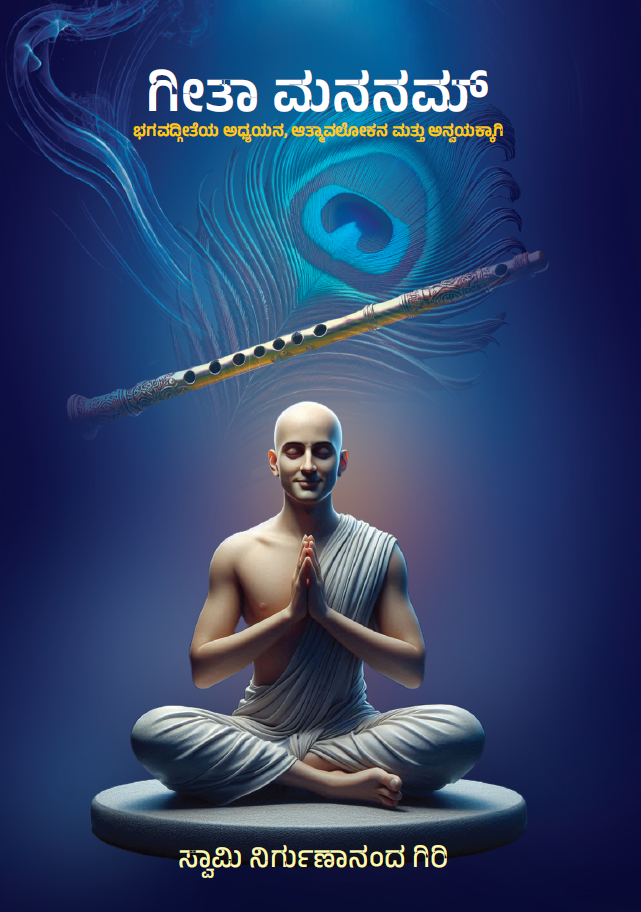
\includegraphics[width=\paperwidth,height=\paperheight]{./images/frontcover.png}%
    }%
}
    \begin{center}
        \vspace*{0.5cm}
            
        {\Huge
        %\textbf{\color{white}\fontsize{50}{60}\selectfont ಗೀತಾ ಮನನಂ}
		}
        %\textbf{\\ \small \color{white}ದೈನಂದಿನ ಸ್ಪೂರ್ತಿ ಹಾಗೂ ಆತ್ಮಾವಲೋಕನಕ್ಕಾಗಿ}    
        \vspace{1.0cm}
            
        
		
            
        \vfill
            
        
            
        \vspace{0.1cm}
        {\color{white}    
		%\textbf{{\Large \mananamfont ಸ್ವಾಮಿ ನಿರ್ಗುಣಾನಂದ ಗಿರಿ}}\\
		%{\normalsize Swami Nirgunananda Giri\\Rishikesh, India}
		}
    \end{center}
\end{titlepage}
\nopagecolor% Use this to restore the color pages to white
\begin{titlepage}
	%\pagecolor{pastelblue}
	%\AddToShipoutPictureBG*{%
    %\AtPageLowerLeft{%
    %    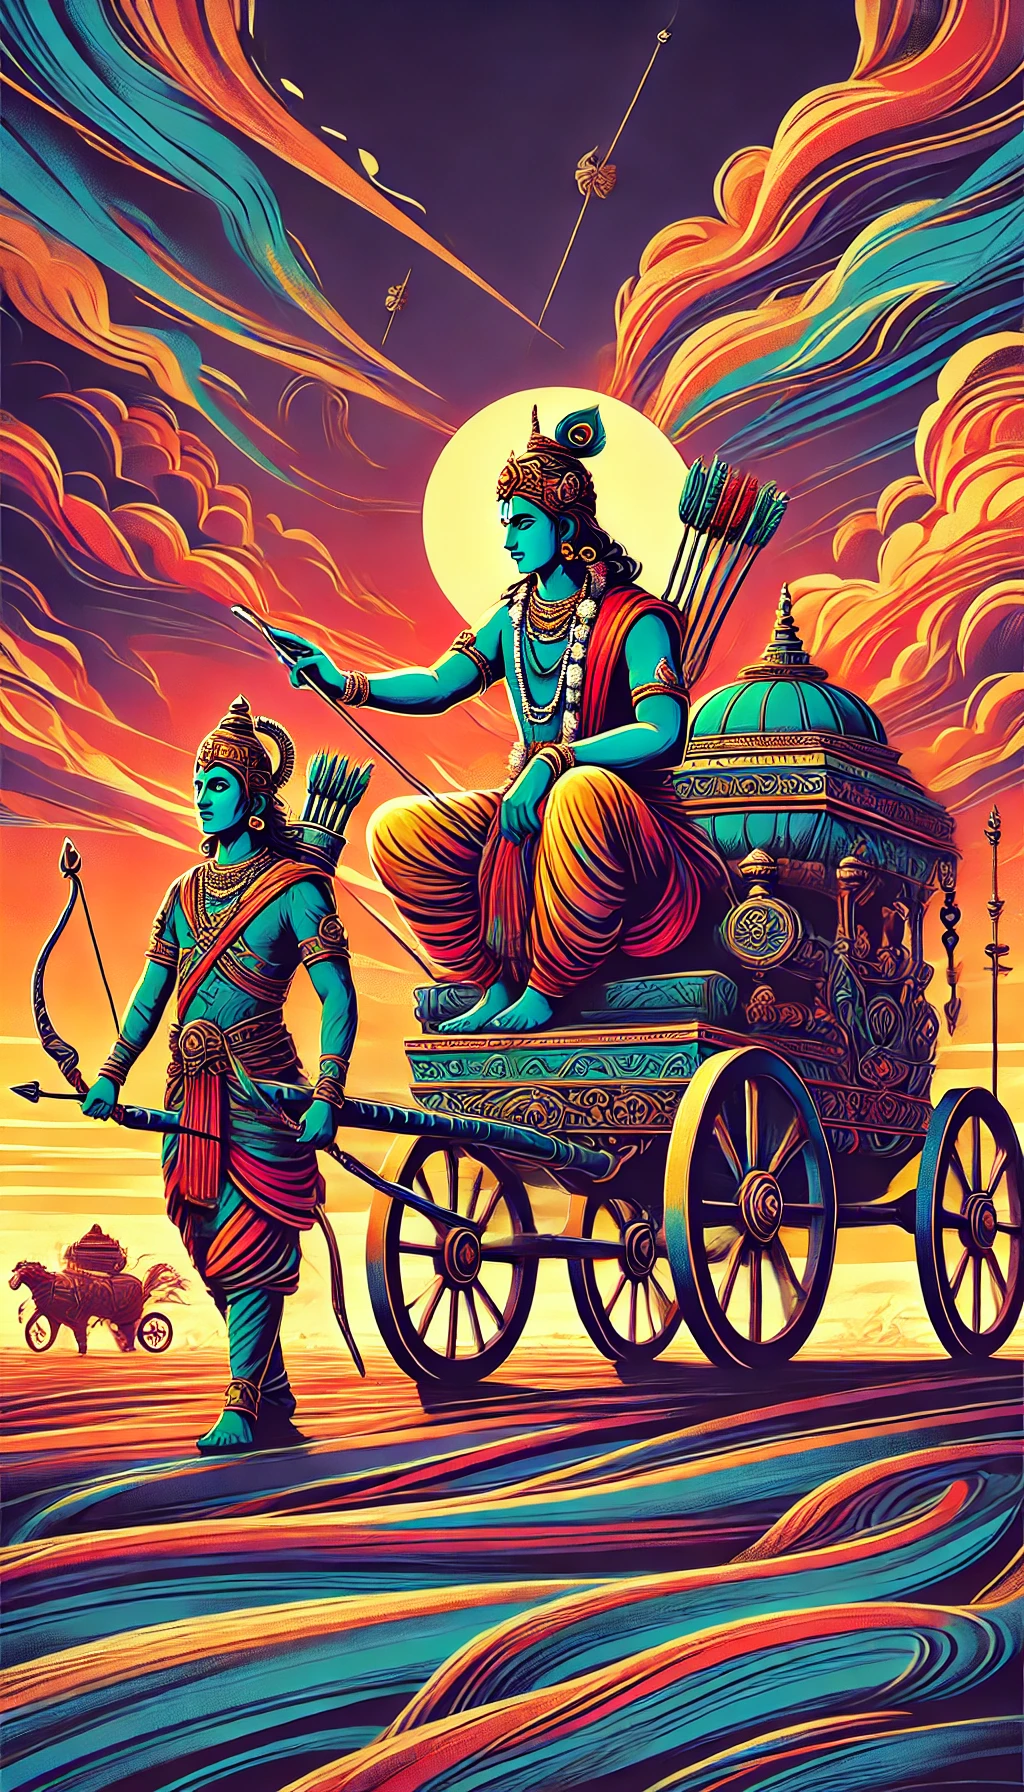
\includegraphics[width=\paperwidth,height=\paperheight]{./images/krishna4.jpg}%
    %}%
%}
    \begin{center}
        \vspace*{0.5cm}
            
        {\Huge
        \textbf{\color{blue}\fontsize{50}{60}\selectfont ಗೀತಾ ಮನನಂ}}
        \textbf{\\ \small \color{black}ದೈನಂದಿನ ಸ್ಪೂರ್ತಿ ಹಾಗೂ ಆತ್ಮಾವಲೋಕನಕ್ಕಾಗಿ}\\    
        \vspace{1.0cm}
		    \textbf{{\large \color{black} ಅಧ್ಯಾಯ ೫ ಕರ್ಮ ಸನ್ಯಾಸ ಯೋಗ}}\\		
        \vspace{6.0cm}
        \textbf{{\Large \color{blue}\mananamfont ಸ್ವಾಮಿ ನಿರ್ಗುಣಾನಂದ ಗಿರಿ}}\\    
        
		
            
        \vfill
            
        
            
        \vspace{0.1cm}
        {\color{black}    
		
		{{\large \color{blue}ಹೃಷೀಕೇಶ, ಉತ್ತರಾ ಖಂಡ}\\\normalsize ಭಾರತ}
        }
    \end{center}
\end{titlepage}
\nopagecolor% Use this to restore the color pages to white
%\maketitle

\thispagestyle{empty}
Copyright \textcopyright\ Swamy Nirgunanandagiri\\
\\
All rights reserved\\
\\
Edition - First, 2024\\
\vfill
Without written permission of the author it is forbidden to reproduce or adapt in any form or by any means any part of this  publication.\\
\\
Rishikesh, India\\
\newpage
\thispagestyle{empty}
\frontmatter

\doublespacing
\tableofcontents
\singlespacing
%\clearpage
%\newgeometry{margin=0pt} % Apply margin only for this page
%\thispagestyle{empty}
%\begin{center}
%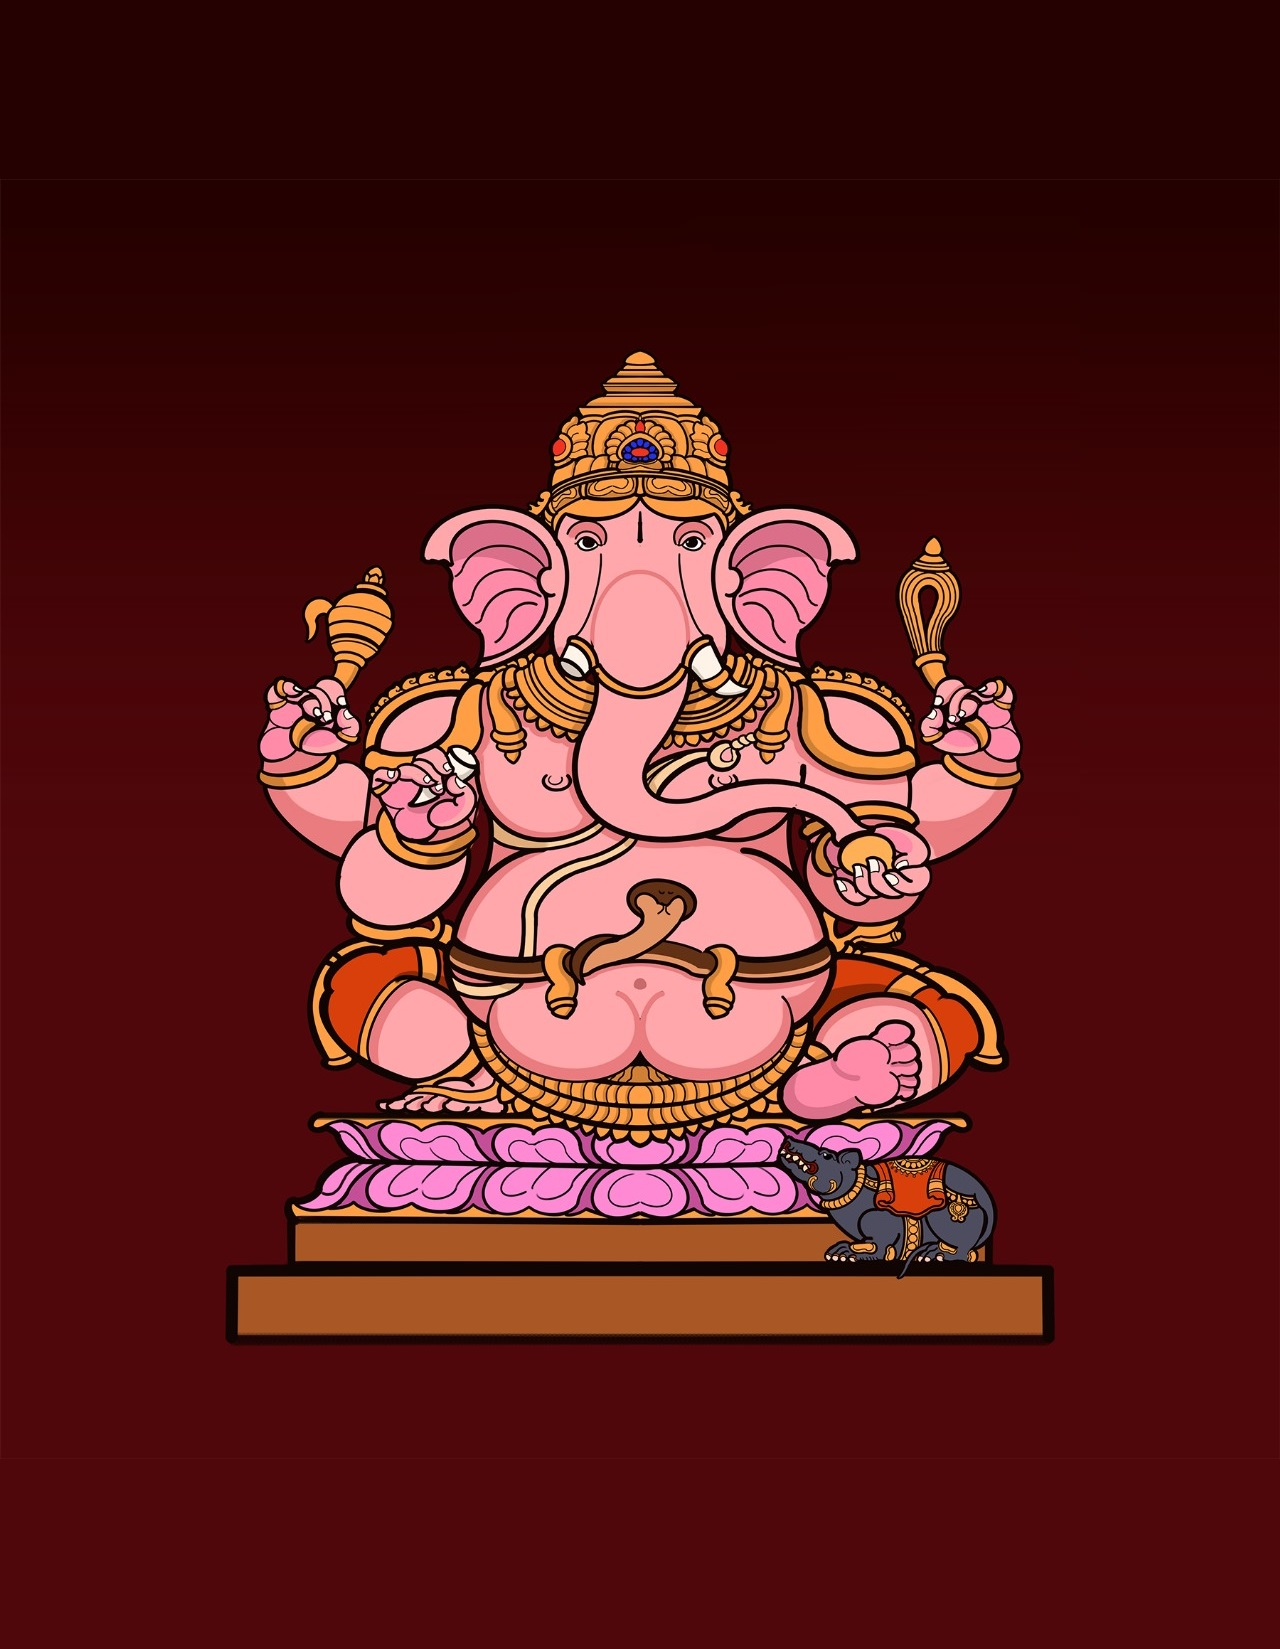
\includegraphics[width=0.9\textwidth, height=\paperheight, keepaspectratio]{./images/ganapa.jpg}
%\end{center}
%\restoregeometry % Restore original geometry settings
%\newpage

\clearpage
\newgeometry{margin=0pt} % Apply margin only for this page
\thispagestyle{empty}
%\begin{figure}
%\centering
%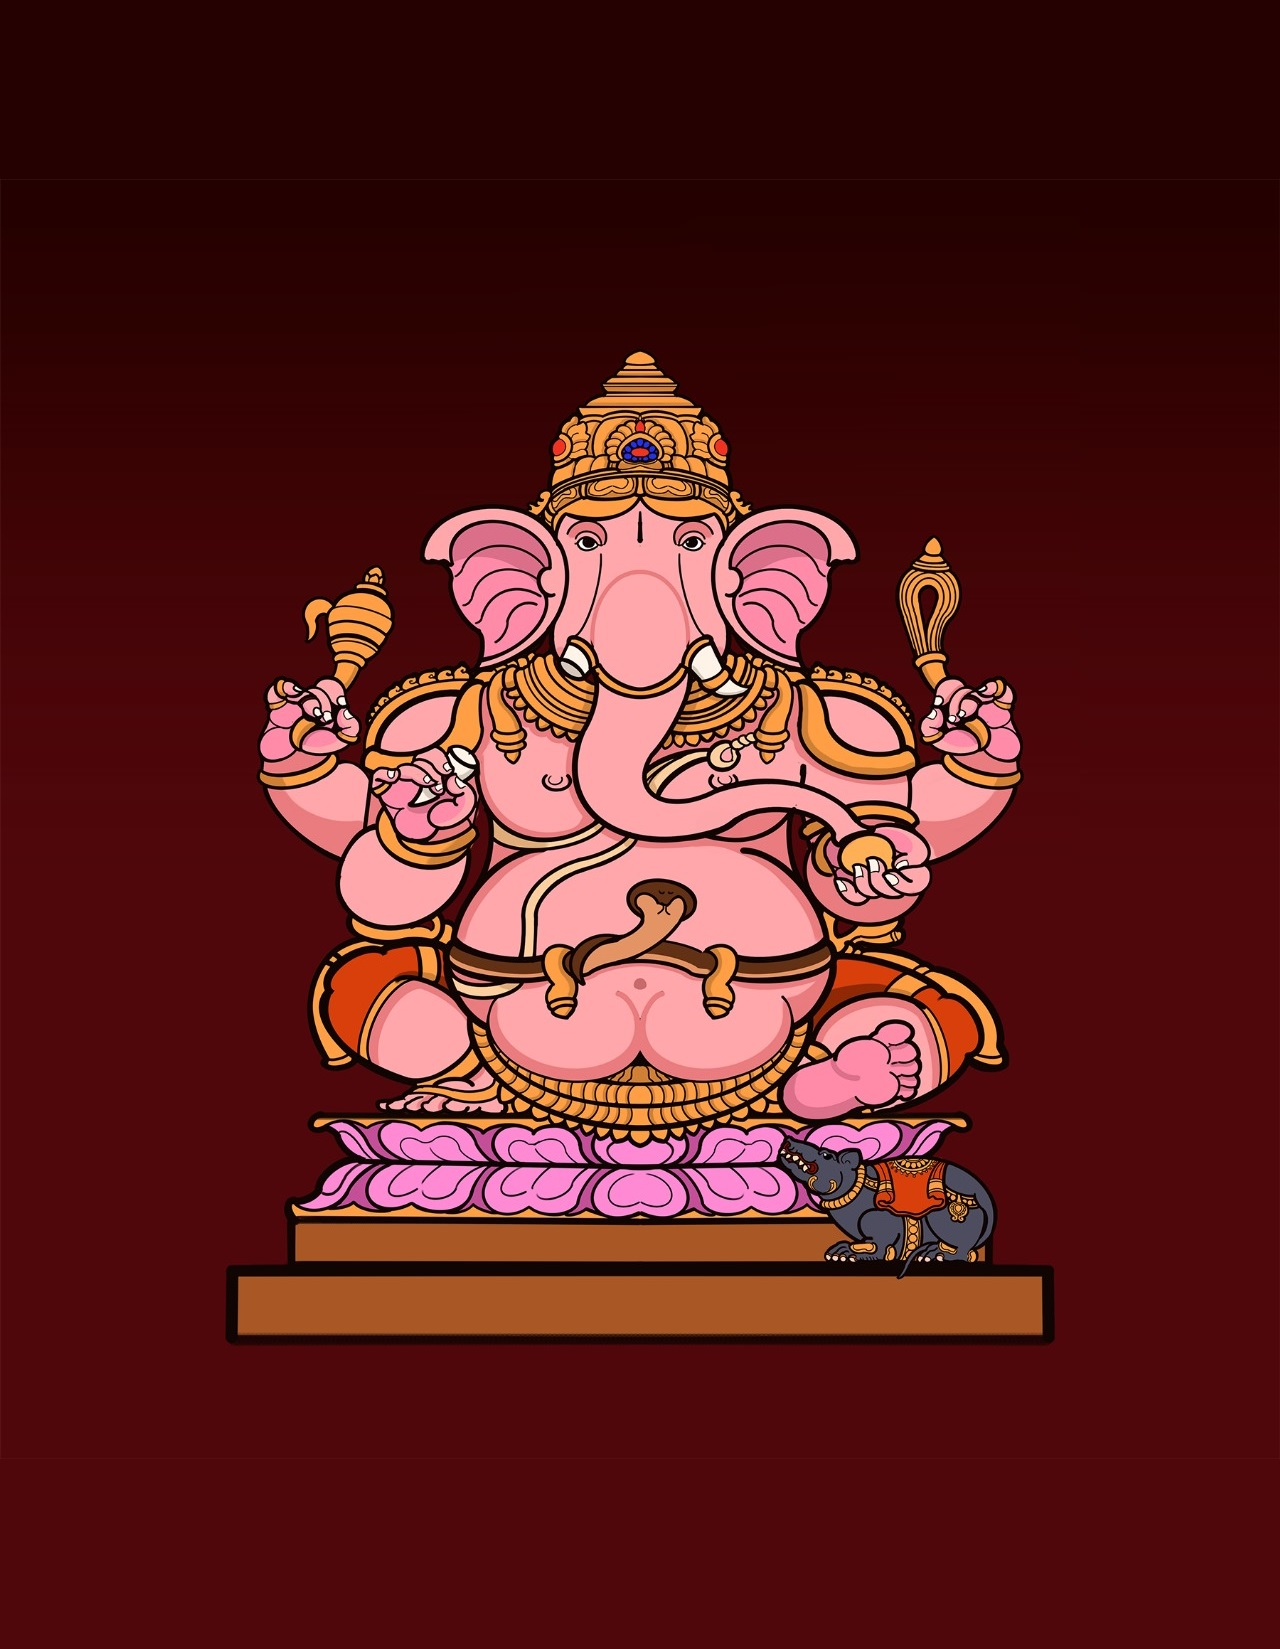
\includegraphics[width=0.9\textwidth, height=\paperheight, keepaspectratio]{./images/ganapa.jpg}
%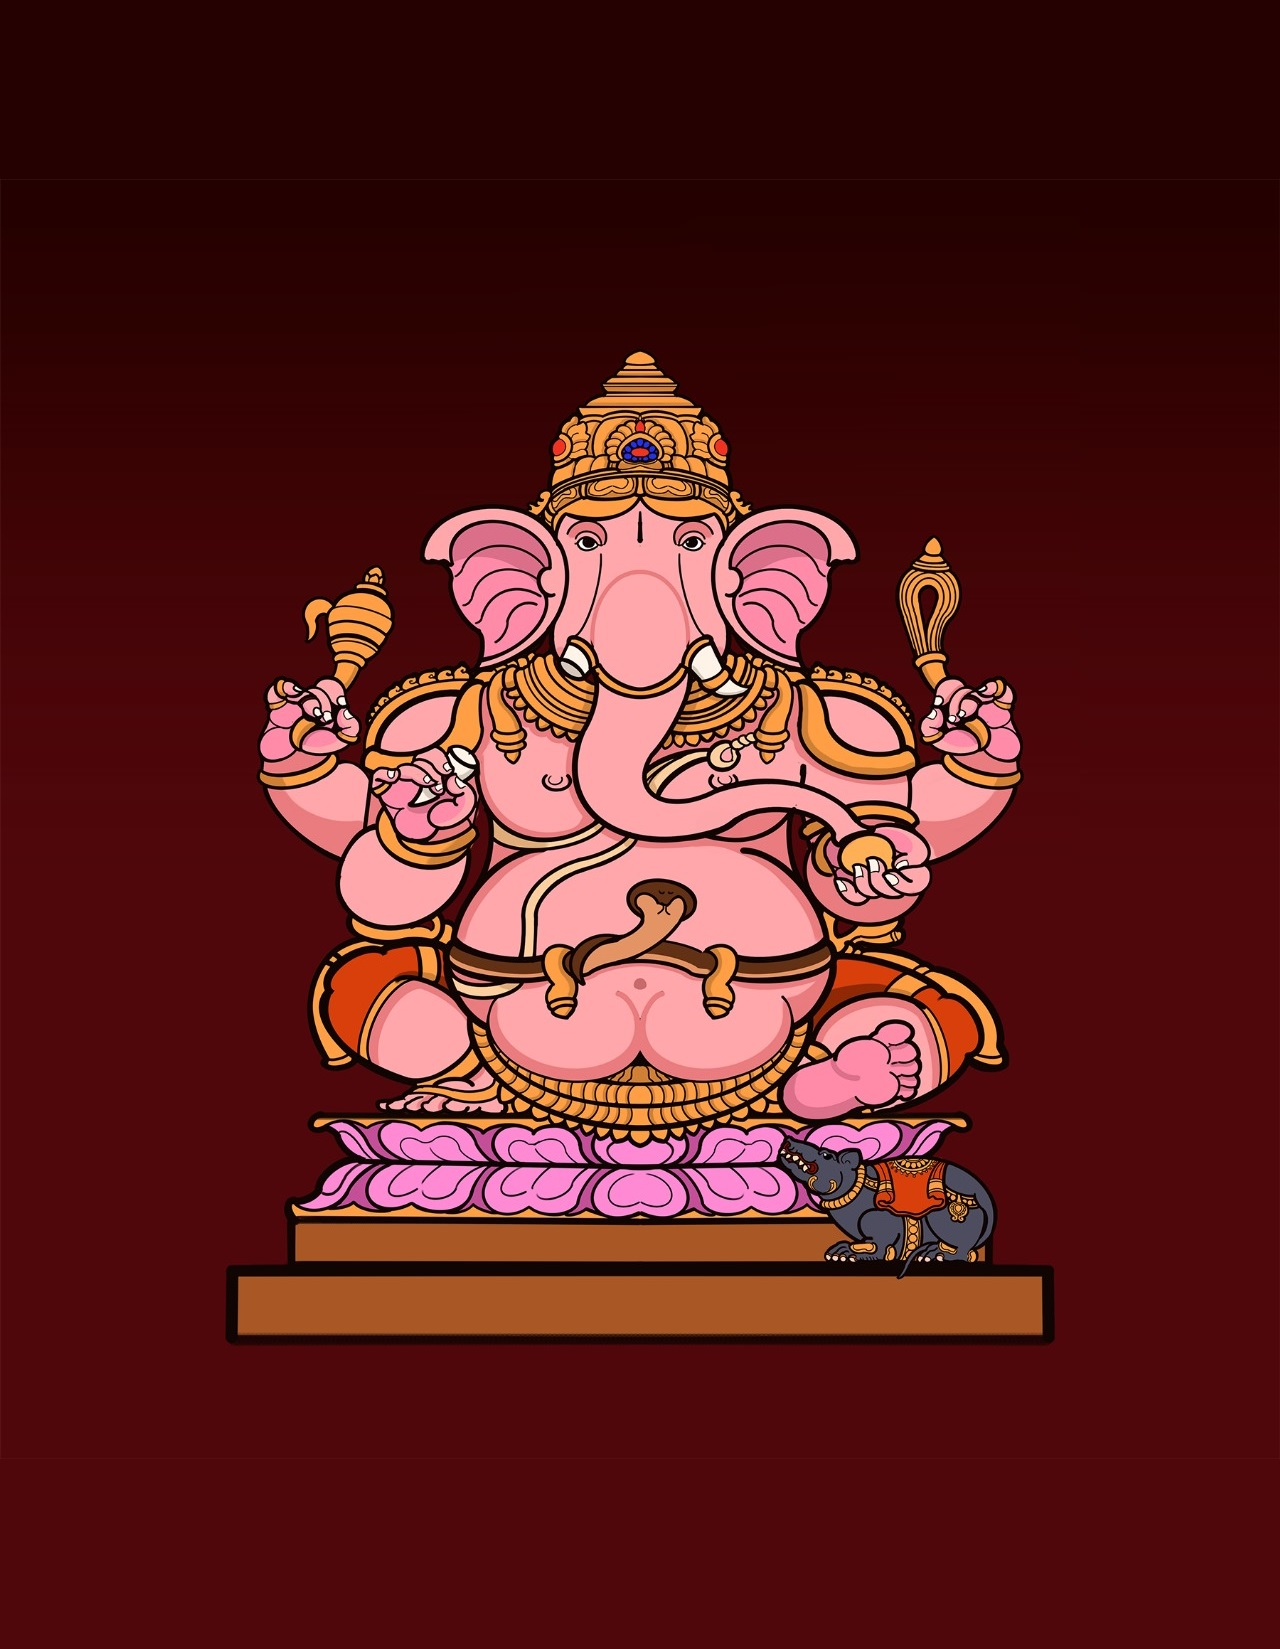
\includegraphics[width=\paperwidth, height=\paperheight]{./images/ganapa.jpg}
%\end{figure}
%\restoregeometry % Restore original geometry settings
%\newpage

\begin{figure}[h!]
    \centering
    \begin{overpic}[width=\paperwidth, height=\paperheight]{../images/001.jpg}
        \put(13,85){\color{white}\kanfont ಗಜಾನನಂ ಭೂತಗಣಾದಿ ಸೇವಿತಂ ಕಪಿತ್ಥ ಜಂಬೂಫಲಸಾರ ಭಕ್ಷಿತಮ್। }\put(10,82){\color{white}\kanfont ಉಮಾಸುತಂ ಶೋಕ ವಿನಾಶಕಾರಣಂ ನಮಾಮಿ ವಿಘ್ನೇಶ್ವರ ಪಾದಪಂಕಜಮ್॥ }
    \end{overpic}
    \caption{This is the standard figure caption below the image.}
    \label{fig:example}
\end{figure}

\restoregeometry

\thispagestyle{empty}
\thispagestyle{empty}
\pagestyle{fancy}


\chapter{\kanfont ಮುನ್ನುಡಿ}
\begin{center}
ದಿಶಂತು ಶಂ ಮೇ ಗುರುಪಾದಪಾಂಸವಃ ॥\\
\end{center}
\footnotesize \mananamtext{ಶ್ರಿ\!\char"0CD5ಮದ್ ಭಗವದ್ಗೀತೆಯು ಎಲ್ಲಾ ಧರ್ಮಗ್ರಂಥಗಳಲ್ಲಿ ಒಂದು ಅನನ್ಯ ಮತ್ತು ಸಾಟಿಯಿಲ್ಲದ ರತ್ನವಾಗಿದೆ.  ಇದು ಪರಿತ್ಯಾಗ ಮಾಡುವವರಿಗೆ ಮಾತ್ರವಲ್ಲದೆ ಲೌಕಿಕ ಜವಾಬ್ದಾರಿಗಳನ್ನು ಹೊತ್ತಿರುವವರಿಗೂ ಮಾರ್ಗದರ್ಶಿ ಬೆಳಕಾಗಿ ಕಾರ್ಯನಿರ್ವಹಿಸುತ್ತದೆ, ಆಧ್ಯಾತ್ಮಿಕದೊಂದಿಗೆ ಪ್ರಾಪಂಚಿಕತೆಯನ್ನು ಸಮತೋಲನಗೊಳಿಸಲು ಪ್ರಯತ್ನಿಸುತ್ತದೆ; ಇದು, ಅಜ್ಞಾನದಿಂದ ಅವರು (ಸಾಮಾನ್ಯ ಜನ) ತಮ್ಮನ್ನು ತಾವು,   ದೇಹ ಮತ್ತು ಮನಸ್ಸಿನ ವ್ಯವಹಾರಗಳ  ಜೊತೆ ಗುರುತಿಸಿಕೊಂಡಾಗ, ಅಂತಹ ವ್ಯವಹಾರಗಳ ಬಗ್ಗೆ ನಿಷ್ಪಕ್ಷಪಾತವಾಗಿರುವಂತೆ ಪ್ರತಿಪಾದಿಸುತ್ತದೆ.\\
ಜೀವನದಲ್ಲಿ ಒಬ್ಬರ ಕರ್ತವ್ಯಗಳನ್ನು ಸಾಧಿಸಲು, ಬಾಂಧವ್ಯದ ಅಥವಾ, ಮೋಹದ ಭಾವನೆ ಇರಬೇಕು ಎಂಬುದು ಒಂದು ತಪ್ಪು ಕಲ್ಪನೆ.  ಭಗವಾನ್ ಕೃಷ್ಣ, ಎಲ್ಲರಿಗಿಂತಲೂ  ದೊಡ್ಡ ಸಂಸಾರಿ ಹಾಗೂ, ಪರಿಪೂರ್ಣವಾದ ಮೋಹರಹಿತನಾದ ಅಸಂಸಾರಿ; ದಿವ್ಯವಾದ ಆನಂದದಲ್ಲಿ ನೆಲೆಗೊಂಡು, ಈ ಮೂರ್ತ, ಭೌತಿಕ ಜಗತ್ತಿನಲ್ಲಿ ಹೇಗೆ ಕಾರ್ಯನಿರ್ವಹಿಸಬೇಕು ಎಂಬುದನ್ನು ಅವನು ತನ್ನ ಕಾರ್ಯಗಳು, ಭಾವ ಮತ್ತು ಅವನು ಉಚ್ಛರಿಸುವ ಪ್ರತಿಯೊಂದೂ ಪರಮಪದದ  ಮೂಲಕ ಪ್ರದರ್ಶಿಸುತ್ತಾನೆ. ಆರಂಭದಲ್ಲಿ ‘ಸಂಘರ್ಷ ಮತ್ತು ಸವಾಲುಗಳಿಂದ ತುಂಬಿರುವ ಮಾರ್ಗ’ ಎಂದು ಕಂಡುಬoದರೂ ಸಹ, ಈ ಸ್ಥಿತಿಯನ್ನು ಸಾಧಿಸಲು (ದಿವ್ಯವಾದ ಆನಂದದಲ್ಲಿ ನೆಲೆಗೊಂಡು, ಈ ಮೂರ್ತ, ಭೌತಿಕ ಜಗತ್ತಿನಲ್ಲಿ  ಕಾರ್ಯನಿರ್ವಹಿಸುವುದು) ಸಮರ್ಥ ಶಿಕ್ಷಕರಿಂದ ಸರಿಯಾದ ಮಾರ್ಗದರ್ಶನದ ಅಗತ್ಯವಿದೆ. \\
ಈ ‘ನಿಪುಣ ಮಾರ್ಗದರ್ಶಿ ಕೈಪಿಡಿ’ಯಲ್ಲಿ, ಲೇಖಕರ ಆಳವಾದ ಒಳನೋಟದಿಂದ ಅಧ್ಯಾಯ 2 ರ 52-53 ಪದ್ಯಗಳಲ್ಲಿ ಸೂಚಿಸಿದಂತೆ: “ಶಿಕ್ಷಕರ ಮತ್ತು ಧರ್ಮಗ್ರಂಥಗಳ ಉದ್ದೇಶವು ನಮ್ಮನ್ನು ಭ್ರಮೆಯಿಂದ ಜಗ್ಗಿಸಿ, ಮುಕ್ತರನ್ನಾಗಿ ಮಾಡುವುದೇ ಆಗಿದೆ. ನಾವು ನಮ್ಮ ಲೌಕಿಕ ಚಿಂತನೆಯ ಮಾದರಿಗಳನ್ನು ಬಿಟ್ಟು, ಒಂದು ಉನ್ನತ ಸತ್ಯದಲ್ಲಿ (ಪಾರಮಾರ್ಥಿಕದಲ್ಲಿ) ಆಶ್ರಯ ಪಡೆಯಲು ಪ್ರಾರಂಭಿಸುತ್ತಿದ್ದಂತೆಯೇ, ಆಧ್ಯಾತ್ಮಿಕ ಪ್ರಯಾಣದ ಒಂದು ಭಾಗವಾದ ಗೊಂದಲಗಳು ಮತ್ತು ಸವಾಲುಗಳು ಏಳುತ್ತವೆ; ಆದರೆ, ನಾವು ಹೀಗೆ ಈ ಹಾದಿಯಲ್ಲಿ ಪ್ರಗತಿ ಹೊಂದುತ್ತಿದ್ದಂತೆ, ಸ್ಪಷ್ಟತೆ ಪಡೆಯಲು ಪ್ರಾರಂಭಿಸುತ್ತೇವೆ”.\\
ಈ ಪುಸ್ತಕವು ಲೇಖಕರ ಕ್ರಾಂತಿಕಾರಿ ಚಿಂತನೆಗಳ ಮೂಲಕ ಓದುಗರನ್ನು ದೇಹದಿಂದ, ಮನಸ್ಸಿಗೆ ಮತ್ತು ಮನಸ್ಸಿನಿಂದ ಪ್ರಜ್ಞೆಗೆ (ಚೈತನ್ಯಕ್ಕೆ), ಒಬ್ಬರ ಅಸ್ತಿತ್ವದ ಪದರಗಳನ್ನು ಭೇದಿಸುವಂತೆ ಮಾಡುತ್ತದೆ. \\
ಪ್ರತಿ ವಿಭಾಗದಲ್ಲಿ, ‘ಮನನಂ’ ಶೀರ್ಷಿಕೆಯಡಿಯಲ್ಲಿರುವ ಆತ್ಮಾವಲೋಕನದ ಪ್ರಶ್ನೆಗಳು, ಸ್ವಯಂ ಸಮಾಧಾನ ಮತ್ತು ಆತ್ಮವಂಚನೆಯಲ್ಲಿ (ಆತ್ಮ ಪ್ರವಂಚನ) ತೊಡಗಿರುವವರಿಗೆ ಯಾವುದೇ ವಿರಾಮ ನೀಡುವುದಿಲ್ಲ ಮತ್ತು ಪ್ರಾಮಾಣಿಕವಾದ ಸ್ವಯಂ ಮೌಲ್ಯಮಾಪನ ಮಾಡಲು ಅವರಿಗೆ ಸವಾಲು ಒಡ್ಡುತ್ತವೆ .  ಮತ್ತೊಂದೆಡೆ, ‘ಸ್ಫೂರ್ತಿ’ಯ ಅಡಿಯಲ್ಲಿರುವ ಪದಗಳು, ಪ್ರಯಾಸಕರ ಮತ್ತು ಗೊಂದಲಮಯ ಆಧ್ಯಾತ್ಮಿಕ ಮಾರ್ಗವನ್ನು ತುಲನಾತ್ಮಕವಾಗಿ ಸುಲಭಗೊಳಿಸಿ, ಸಕಾರಾತ್ಮಕತೆಯ ಒಂದು, ಅಕ್ಷಯವಾದ ಮೂಲವಾಗಿ ಕಾರ್ಯನಿರ್ವಹಿಸುತ್ತವೆ.\\
ಈ ಕೈಪಿಡಿಯು, ಆಕಾಂಕ್ಷಿಗಳಿಗೆ ಜೀವನದ ವಿವಿಧ ಸಮಸ್ಯೆಗಳಿಗೆ ಪರಿಹಾರವನ್ನು ಕಂಡುಕೊಳ್ಳಲು ಸಾಕಷ್ಟು ಸಮಾಧಾನಗಳನ್ನು  ನೀಡುತ್ತದೆ, ಆದರೆ ಬಾಹ್ಯವಾಗಿ ಅಲ್ಲ, ಆಂತರಿಕವಾಗಿ.\\
ಈ ಪುಸ್ತಕದ ವಿಷಯವು, ‘ಮಾನವ ಮನೋವಿಜ್ಞಾನ’ದ ಬಗ್ಗೆ ಲೇಖಕರ ಆಳವಾದ ತಿಳುವಳಿಕೆಯನ್ನು ತೋರಿಸುತ್ತದೆ, ಮೊದಲು ಸಕಾರಾತ್ಮಕ ಮಾನಸಿಕ ಸ್ಥಿತಿಯ ಕಡೆಗೆ ಮತ್ತು ನಂತರ ಅದನ್ನು ಮೀರಿ, ಆಂತರಿಕ ಶಾಶ್ವತವಾದ ಆತ್ಮದೆಡೆಗೆ, ಸರಳವಾಗಿ ಮುಂದುವರಿಯುತ್ತದೆ. \\
ಈ ಪುಸ್ತಕದ ಓದುಗರು ಈ ಪ್ರಯಾಣವನ್ನು ಪ್ರಾರಂಭಿಸಿದಾಗ, ಅವರು ಖಂಡಿತವಾಗಿಯೂ ಮಾನವ ಮನಸ್ಸಿನ ಕ್ಷೇತ್ರವನ್ನು ಮೀರುತ್ತಾರೆ ಮತ್ತು ಈ ಸ್ವರ್ಗೀಯ ಗೀತೆಯಾದ  ‘ಭಗವದ್ಗೀತೆ’ ಗಾಯಕನ ಕೃಪೆಯಿಂದ ‘ಅಧಿಷ್ಠಾನ ಚೈತನ್ಯಮ್’ (ಚೇತನಾತ್ಮಕದ ಅಂತಿಮ ಮೂಲತತ್ವ) ಅನ್ನು ತಲುಪುತ್ತಾರೆ. ಸಾಧಕರ ಅನುಕೂಲಕ್ಕಾಗಿ ತಮ್ಮ ಅಮೂಲ್ಯವಾದ ಆಲೋಚನೆಗಳನ್ನು ಲೇಖಿಸಿದ, ಸ್ವಾಮಿ ನಿರ್ಗುಣಾನಂದ ಗಿರಿ, ಇವರ ನಿಸ್ವಾರ್ಥ ಪ್ರಯತ್ನವನ್ನು,  ಸನಾತನ ಗುರುವಾದ, ಆ ಭಗವಂತ ಶ್ರೀಕೃಷ್ಣನು ಆಶೀರ್ವದಿಸಲಿ.\\\\
\begin{center}
ಮಂಗಳಂ ಸರ್ವಂ
\end{center}

{\kanBold ಸ್ವಾಮಿ ಸ್ವಾನಂದ ತೀರ್ಥ} \\
ಆಚಾರ್ಯ, ಕೈಲಾಸ್ ಆಶ್ರಮ\\
ಋಷಿಕೇಶ – ಉತ್ತರಖಂಡ\\
}
%\thispagestyle{empty}
\begin{onehalfspace}
\chapter{\kanfont ಪ್ರಸ್ತಾವನೆ}
\footnotesize \mananamtext{ನಾವೆಲ್ಲರೂ ಜೀವನದ ಹೋರಾಟಗಳನ್ನು ಎದುರಿಸಲೇಬೇಕು. ಕುರುಕ್ಷೇತ್ರ ಯುದ್ಧದಲ್ಲಿ ಶ್ರೀ ಕೃಷ್ಣ ಪರಮಾತ್ಮನು, ತನ್ನ ವೇದನಾಯುಕ್ತ ಶಿಷ್ಯ ಅರ್ಜುನನಿಗೆ, ಪ್ರಾಪಂಚಿಕತೆಯಲ್ಲಿಯೂ ಅಧ್ಯಾತ್ಮಿಕತೆಯನ್ನು ಆಚರಣೆಗೆ ತರುವಂತಹ, ಸಂಕ್ಷಿಪ್ತ ಹಾಗೂ ಪ್ರಾಯೋಗಿಕವಾದ,  ಅತೀ ಪವಿತ್ರವಾದ ಬೋಧನೆಗಳನ್ನು ಕೊಟ್ಟಿದ್ದಾನೆ. ಈ ಶ್ರೇಷ್ಠವಾದ ಉಪನಿಷತ್ತುಗಳ ಸತ್ವಗಳನ್ನೊಳಗೊಂಡ  ಬೋಧನೆಗಳನ್ನು ಪವಿತ್ರವಾದ, ‘ಭಗವದ್ಗೀತ, ಒಂದು ಪವಿತ್ರ ಗಾನ’ ದ ಸ್ವರೂಪದಲ್ಲಿ, ಋಷಿ ವೇದವ್ಯಾಸರು ನಮಗೆ ನೀಡಿರುವ ಅಸೀಮವಾದ ಕೊಡುಗೆ. \\
 ಅರ್ಜುನನು ಇದ್ದ ಪರಿಸ್ಥಿತಿಗೂ, ನಾವು ಇರುವ ಪರಿಸ್ಥಿತಿ ಮತ್ತು ಸಂಘರ್ಷಗಳಿಗೂ ವ್ಯತ್ಯಾಸಗಳಿರಬಹುದು. ಆದರೆ, ಗೀತೆಯ ಸಾರ್ವತ್ರಿಕ ಉಪದೇಶಗಳು ಸತ್ಯಾನ್ವೇಷಣೆ ಮಾಡಲು ಬಯಸುವ ಪ್ರತಿಯೊಬ್ಬನಿಗೂ ಆತ್ಮೋನ್ನತಿ  ಮತ್ತು ಅಧ್ಯಾತ್ಮಿಕ ಪ್ರಗತಿ ಸಾಧಿಸಲು ಬೇಕಾಗುವ ಮಾದರಿಯಾಗಿದೆ.\\
 ಭಗವದ್ಗೀತೆಯ ಉಪದೇಶಗಳು ಕೇವಲ ಆಧ್ಯಾತ್ಮಿಕ ಅನ್ವೇಷಣೆ ಮಾಡುವವರಿಗೆ ಸಮರ್ಪಿತವಾದದ್ದು ಮಾತ್ರವೇ ಅಲ್ಲ, ಜೀವನಕ್ಕೆ ಬೇಕಾಗುವ ಅತ್ಯಮೂಲ್ಯವಾದ ಕೈಪಿಡಿಯೂ ಆಗಿದೆ. ಯಾರು, ಕೆಲಸದಲ್ಲಿ ಮತ್ತು ಕೌಟುಂಬಿಕ ಜವಾಬ್ದಾರಿಗಳಲ್ಲಿ ಒತ್ತಡ ರಹಿತವಾಗಿ, ಸಮತೋಲನ ಮತ್ತು ಮಾನಸಿಕ ನೆಮ್ಮದಿ ಕಾಪಾಡಿಕೊಳ್ಳಲು  ಬಯಸುತ್ತಾರೋ ಅವರಿಗೆ ಈ ಬೋಧನೆಗಳು ಬಹಳ ಮಹತ್ವದ್ದಾಗಿರುತ್ತವೆ. \\
 ಅನೇಕ ಗುರುಗಳು ಮತ್ತು ವಿದ್ವಾಂಸರು ಈಗಾಗಲೇ ಮಾಡಿರುವಂತೆ ಈ ದಿನಚರಿ ಪುಸ್ತಕ ಮತ್ತು ನಿಯತಕಾಲಿಕವು, ಗೀತೆಯ ಬೋಧನೆಗಳನ್ನು ತಿಳಿಸುವ ಪ್ರಯತ್ನ ಅಥವಾ ವ್ಯಾಖ್ಯಾನ ಕೊಡುವುದಾಗಿಲ್ಲ. ಈ ಗೀತಾ ಮನನವು, ಬೋಧನೆಗಳ ಚಿಂತನೆ ಮಾಡುವುದು ಮತ್ತು ಅದನ್ನು ನಮ್ಮ ಸ್ವಂತದ್ದನ್ನಾಗಿ ಅಂದರೆ, ಜೀವನದಲ್ಲಿ ಅಳವಡಿಸಿಕೊಳ್ಳಲು ಸುಲಭವಾಗುವಂತೆ ಮಾಡಿಕೊಳ್ಳುವುದೇ ಆಗಿದೆ. ದೇವ ನಾಗರಿಯಲ್ಲಿರುವ `ಮನನ` ಎಂಬ ಪದವು ಆಗಲೇ ಕೇಳಿದ್ದನ್ನು ಅಥವಾ ಓದಿದ್ದನ್ನು ಚಿಂತನೆ ಮಾಡುವ ಕಾರ್ಯವಿಧಾನವನ್ನು ಅನ್ವಯಿಸುವುದಾಗಿದೆ.\\
 ಈ ದಿನಚರಿ ಪುಸ್ತಕವನ್ನು ನೀವು, ನಿಮ್ಮ ಮನಸ್ಸಿನ ಇಂಗಿತವನ್ನು ಸ್ವತಂತ್ರವಾಗಿ ವ್ಯಕ್ತಪಡಿಸಲು  ಮತ್ತು ನಿಮ್ಮ ಜೀವನದಲ್ಲಿ ಅಳವಡಿಸಿಕೊಳ್ಳಲು ಅವಕಾಶ ಮಾಡಿಕೊಡುವ ಸಲುವಾಗಿ  ರೂಪಿಸಲಾಗಿದೆ. ಗೀತೆಯಲ್ಲಿರುವ ಶ್ಲೋಕಗಳ ಆಧಾರದ ಮೇಲೆ ರಚಿಸಲಾಗಿರುವ ಈ ಪ್ರಶ್ನೆಗಳು, ಆಯಾ ಬೋಧನೆಗಳ ಸನ್ನಿವೇಶಕ್ಕೆ ತಕ್ಕಂತೆ, ನಿಮ್ಮ ವೈಯಕ್ತಿಕ ಅರ್ಥಗಳನ್ನು ಹುಡುಕಲು ಮತ್ತು ಅದರಿಂದ ಜೀವನದ ಸಂದರ್ಭದೊಳಗೆ ಅಪಾರ ಸ್ಪಷ್ಟನೆ ದೊರಕಿಸಲು ಸಹಾಯಕವಾಗುವಂತೆ ರೂಪಿಸಲಾಗಿದೆ.\\
 ಶ್ರಿ\!\char"0CD5ಕೃಷ್ಣ ಪರಮಾತ್ಮನು  ಅರ್ಜುನನಿಗೆ ಧಾರ್ಮಿಕ ಯುದ್ಧವನ್ನು ಮಾಡಲು ಪ್ರೇರೇಪಿಸಿದಂತೆ, ನಿಮ್ಮ ಜೀವನದ ದಿನನಿತ್ಯದ ಕರ್ತವ್ಯಗಳನ್ನು ಈ “ಗೀತಾ ಮನನಮ್ “ ಮೂಲಕ  ಸಮರ್ಪಕವಾಗಿ ನಿರ್ವಹಿಸಲು,  ಆ ಭಗವಂತ ನಿಮ್ಮನ್ನೂ ಪ್ರೇರೇಪಿಸುತ್ತಾನೆ ಎಂದು ನಂಬುತ್ತೇನೆ. ನಿಮ್ಮ ಅಂತರಂಗದ ಶಾಂತಿ, ವೈಯಕ್ತಿಕ ಪ್ರಗತಿಯನ್ನು ನಿರ್ಲಕ್ಷಿಸದೇ, ನಿಮ್ಮ ಕರ್ತವ್ಯಗಳನ್ನು ಕುಶಲತೆಯಿಂದ ಯಶಸ್ವಿಯಾಗಿ ನಿರ್ವಹಿಸುತ್ತಾ  ಮತ್ತು ನಿಶ್ಚಲವಾಗಿ ದೈವತ್ವದಲ್ಲಿ ಮನಸನ್ನಿಡುವುದೇ, ಈ ದಿವ್ಯವಾದ ಗೀತೆಯ ನಿರಂತರ ಉದ್ದೇಶ.\\
ನಾನು ಈ ಪುಸ್ತಕದಲ್ಲಿ ಬಳಸಿರುವ ಚಿತ್ರಕಲೆ ಮತ್ತು ರೇಖಾಚಿತ್ರಗಳಿಗಾಗಿ ಶ್ರಿ\!\char"0CD5ಯುತ ಕೆ.ಎಂ.ಶೇಷಗಿರಿ ಅವರಿಗೆ ಧನ್ಯವಾದಗಳನ್ನು ಸಲ್ಲಿಸುತ್ತೇನೆ. ನನ್ನ ಗೀತಾ ತರಗತಿಯಲ್ಲಿ ಭಾಗವಹಿಸಿದ್ದ ಅನೇಕ ವಿದ್ಯಾರ್ಥಿಗಳು ಶ್ಲೋಕಗಳ ಭಾಷಾಂತರ, ತಿದ್ದುವಿಕೆ, ಸಂಪಾದನೆ, ವಿನ್ಯಾಸ ಮತ್ತು ಮುದ್ರಣ ಪ್ರಕ್ರಿಯೆಯನ್ನು ಗಮನಿಸುವಲ್ಲಿ ತೊಡಗಿಸಿಕೊಂಡಿದ್ದಾರೆ. ಈ ಗ್ರಂಥವನ್ನು ಓದುಗರ ಹಿತಾರ್ಥಕ್ಕಾಗಿ ಸಮರ್ಪಣೆಯಿಂದ ಮಾಡಿದ ಅವರ ತ್ಯಾಗಮಯ ಸೇವೆಗೆ ಭಗವಂತನ ಕೃಪೆ ಹಾಗು ನನ್ನ ಆಶೀರ್ವಾದಗಳು. \\\\
}
{
\kanBold{ಸ್ವಾಮಿ ನಿರ್ಗುಣಾನಂದ ಗಿರಿ}
}

\end{onehalfspace}
\mainmatter
%\centerline{\textbf{ಅಥ ಪ್ರಥಮೋऽಧ್ಯಾಯಃ ।}\\}
ಮೊಟ್ಟ ಮೊದಲನೆಯ ಶ್ಲೋಕವೇ ನಮಗೆ ಚಿಂತನೆ, ಮನನ ಪ್ರಾರಂಭಿಸಲು ಬೇಕಾಗುವ ಸೂಕ್ಷ್ಮವಾದ ಸಂದೇಶವನ್ನು ಕೊಡುತ್ತದೆ.\\
\slcol{ಧೃತರಾಷ್ಟ್ರ ಉವಾಚ ।\\
\index{ಧರ್ಮಕ್ಷೇತ್ರೇ ಕುರುಕ್ಷೇತ್ರೇ} ಸಮವೇತಾ ಯುಯುತ್ಸವಃ ।\\
ಮಾಮಕಾಃ ಪಾಂಡವಾಶ್ಚೈವ ಕಿಮಕುರ್ವತ ಸಂಜಯ ॥ 1 ॥}
\cquote{ಧೃತರಾಷ್ಟ್ರನು ಹೇಳಿದನು,\\
ಸಂಜಯನೇ, ಯುದ್ಧದ ಬಯಕೆಯಿಂದ ಧರ್ಮಭೂಮಿಯಾದ ಕುರುಕ್ಷೇತ್ರದಲ್ಲಿ ಕಲೆತ ನನ್ನ ಮಕ್ಕಳೂ ಪಾಂಡವರೂ ಏನು ಮಾಡಿದರು?\\}
\slcol{ಸಂಜಯ ಉವಾಚ ।\\
\index{ದೃಷ್ಟ್ವಾ ತು ಪಾಂಡವಾನೀಕಂ} ವ್ಯೂಢಂ ದುರ್ಯೋಧನಸ್ತದಾ ।\\
ಆಚಾರ್ಯಮುಪಸಂಗಮ್ಯ ರಾಜಾ ವಚನಮಬ್ರವೀತ್ ॥ 2 ॥}
\cquote{ಸಂಜಯನು ಹೇಳಿದನು,\\
ಪಾಂಡವರ ದಂಡು ಸಜ್ಜಾಗಿ ನಿಂತಿದ್ದುದನ್ನು ನೋಡಿದ ಅರಸನಾದ ದುರ್ಯೋಧನನು ಗುರುಗಳಾದ ದ್ರೋಣರ ಬಳಿಗೆ ಬಂದು ಹೀಗೆ ಹೇಳಿದನು. \\}
\slcol{\index{ಪಶ್ಯೈತಾಂ ಪಾಂಡುಪುತ್ರಾಣಾಮಾಚಾರ್ಯ} ಮಹತೀಂ ಚಮೂಮ್ ।\\
ವ್ಯೂಢಾಂ ದ್ರುಪದಪುತ್ರೇಣ ತವ ಶಿಷ್ಯೇಣ ಧೀಮತಾ ॥ 3 ॥}
\cquote{ಗುರುಗಳೇ, ದೃಪದರಾಜನ ಮಗ ನಿಮ್ಮ ಶಿಷ್ಯ, ಬುದ್ಧಿಶಾಲಿಯಾದ ದೃಷ್ಟದ್ಯುಮ್ನ ಪಾಂಡವರ ಈ ದೊಡ್ಡ ದಂಡನ್ನು ಸಜ್ಜುಗೊಳಿಸಿರುವುದನ್ನು ನೋಡಿರಿ.\\}
\slcol{\index{ಅತ್ರ ಶೂರಾ ಮಹೇಷ್ವಾಸಾ} ಭೀಮಾರ್ಜುನಸಮಾ ಯುಧಿ ।\\
ಯುಯುಧಾನೋ ವಿರಾಟಶ್ಚ ದ್ರುಪದಶ್ಚ ಮಹಾರಥಃ ॥ 4 ॥}

\newpage
\begin{mananam}{\kanfont ಮನನ ಶ್ಲೋಕ - }
{\footnotesize \mananamfont ನನ್ನ ಜೀವನದ ದೈನಂದಿನ ನಿತ್ಯಕರ್ಮದಲ್ಲಿ ಯಾವಾಗ ನನ್ನ ದೇಹವು, ಆಸೆ, ಕೋಪ, ಭಯ, ಮತ್ಸರ ಇತ್ಯಾದಿಗಳಲ್ಲಿ ಒಲವು ತೋರುವುದನ್ನು ಗುರುತಿಸಿತು, ಅವುಗಳನ್ನು ಸ್ವಾತಂತ್ರ್ಯವನ್ನು ಆಳವಾಗಿ ಪ್ರೇರೇಪಿಸುವ ನನ್ನನ್ನು ಪ್ರತಿಭಟಿಸುವಂತೆ ಮಾಡುವ ಮತ್ತು ಸನಾತನ ಗ್ರಂಥ ಮತ್ತು ಬೋಧಕರಿಂದ ಪಡೆದ ಜ್ಞಾನವನ್ನು ಯಾವ ಬಲವನ್ನು ಅನುಸರಿಸಿದೆ? ನನ್ನ ಹಂಬಲ ಮತ್ತು ಸಂಕಲ್ಪಗಳನ್ನು ತಳ್ಳಿಹಾಕುವ ನನ್ನ ದುರಭ್ಯಾಸಗಳು ಮತ್ತು ಅಪಾಯಕಾರಿ ನಡವಳಿಕೆಗಳಿಂದಾಗಿ ನನ್ನ ನಿತ್ಯ ಜೀವನದಲ್ಲಿ ಏನೇನು ಕಷ್ಟ ಪಡಬೇಕಾಯಿತು?}
\end{mananam}
\WritingHand\enspace\textbf{ಆತ್ಮ ವಿಮರ್ಶೆ}
\begin{inspiration}{\kanfont ಸ್ಪೂರ್ತಿ}
{\footnotesize \mananamfont ನಿನಗೆ ನೀನು ಸತ್ಯವಾಗಿರು ಮತ್ತು ನೀನು ಉನ್ನತಿಯತ್ತ ಬದಲಾಗುವೆ. ಜೀವನದಲ್ಲಿ ಜಾಣನಿಗೆ ಅವಶ್ಯಕವಾದುದು ಪಕ್ಷಪಾತ ರಹಿತ ಅವಲೋಕನ. ನಮ್ಮನ್ನು ನಾವು ಬದಲಾಯಿಸಿಕೊಳ್ಳಲು ಕೇವಲ ಬಯಕೆ ಇದ್ದರೆ ಮಾತ್ರ ಸಾಲದು. ಜ್ಞಾನಿಗಳ ಮಹತ್ವದ, ಉನ್ನತವಾದ ಬೋಧನೆಗಳಿಂದ ನಮ್ಮ ಯೋಚನೆಗಳು, ಮಾತುಗಳು ಮತ್ತು ಕೃತಿಗಳನ್ನು ತಹಬಂದಿಗೆ ತಂದು, ಪ್ರತಿದಿನವೂ ನಮ್ಮನ್ನು ನಾವು ಆತ್ಮ ವಿಮರ್ಶೆ ಮಾಡಿಕೊಳ್ಳಲೇಬೇಕು.}
\end{inspiration}
\newpage

\cquote{ಈ ದಂಡಿನಲ್ಲಿ ಹೋರಾಟದಲ್ಲಿ ಭೀಮಾರ್ಜುನರಿಗೆ ಸರಿ ಜೋಡಿಯಾದ ಶೂರರಾಗಿ ದೊಡ್ಡ ದೊಡ್ಡ ಬಿಲ್ಲುಗಳನ್ನು ಹಿಡಿದುಕೊಂಡು ಕಾದುವುದರಲ್ಲಿ ಕುಶಲರಾದ ಸಾತ್ಯಕಿ ವಿರಾಟರಿದ್ದಾರೆ. ಸಹಸ್ರ ಜನರೊಡನೆ ಏಕಾಂಗಿಯಾಗಿ ಹೋರಾಡಬಲ್ಲ ದ್ರುಪದನಿದ್ದಾನೆ.\\}
\slcol{\index{ಧೃಷ್ಟಕೇತುಶ್ಚೇಕಿತಾನಃ} ಕಾಶಿರಾಜಶ್ಚ ವೀರ್ಯವಾನ್ ।\\
ಪುರುಜಿತ್ಕುಂತಿಭೋಜಶ್ಚ ಶೈಬ್ಯಶ್ಚ ನರಪುಂಗವಃ ॥ 5 ॥}
\cquote{ದೃಷ್ಟಕೇತು, ಚೀಕಿತಾನ, ವೀರನಾದ ಕಾಶಿರಾಜ, ಮತ್ತು ಮನುಷ್ಯರಲ್ಲಿ ಶ್ರೇಷ್ಠನಾದ ಶೈಭ್ಯ ಇವರೆಲ್ಲ ಇದ್ದಾರೆ. \\} 
\slcol{\index{ಯುಧಾಮನ್ಯುಶ್ಚ ವಿಕ್ರಾಂತ} ಉತ್ತಮೌಜಾಶ್ಚ ವೀರ್ಯವಾನ್ ।\\
ಸೌಭದ್ರೋ ದ್ರೌಪದೇಯಾಶ್ಚ ಸರ್ವ ಏವ ಮಹಾರಥಾಃ ॥ 6 ॥}
\cquote{ಬಲಶಾಲಿಯಾದ ಯುಧಾಮನ್ಯು, ವೀರನಾದ ಉತ್ತಮೌಜ, ಸುಭದ್ರೆಯ ಮಗ ಅಭಿಮನ್ಯು ಮತ್ತು ದ್ರೌಪದಿಯ ಮಕ್ಕಳು ಇದ್ದಾರೆ. ಎಲ್ಲರೂ ಒಬ್ಬೊಬ್ಬರು ಹತ್ತು ಸಹಸ್ರ ಜನರೊಡನೆ ಹೋರಾಡಬಲ್ಲ ಮಹಾರುತರು. \\}
\slcol{\index{ಅಸ್ಮಾಕಂ ತು ವಿಶಿಷ್ಟಾ ಯೇ} ತಾನ್ನಿಬೋಧ ದ್ವಿಜೋತ್ತಮ ।\\
ನಾಯಕಾ ಮಮ ಸೈನ್ಯಸ್ಯ ಸಂಙ್ಞಾರ್ಥಂ ತಾನ್ಬ್ರವೀಮಿ ತೇ ॥ 7 ॥}
\cquote{ಬ್ರಾಹ್ಮಣ ಶ್ರೇಷ್ಠರೇ, ನಮ್ಮ ಕಡೆಯಲ್ಲಿರುವ ವೀರರನ್ನು ನೆನಪಿಗೆ ತಂದುಕೊಳ್ಳಿ. ತಮಗೆ ನೆನಪಾಗಲೆಂದು ಅವರ ಹೆಸರುಗಳನ್ನು ಹೇಳುತ್ತೇನೆ.\\} 
\slcol{\index{ಭವಾನ್ಭೀಷ್ಮಶ್ಚ ಕರ್ಣಶ್ಚ} ಕೃಪಶ್ಚ ಸಮಿತಿಂಜಯಃ ।\\
ಅಶ್ವತ್ಥಾಮಾ ವಿಕರ್ಣಶ್ಚ ಸೌಮದತ್ತಿಸ್ತಥೈವ ಚ ॥ 8 ॥}
\cquote{ತಾವು ಭೀಷ್ಮ ಕರ್ಣ ಜಯಶೀಲನಾದ ಕೃಪಾ, ಅಶ್ವತ್ಥಾಮ, ವಿಕರ್ಣ ಸೋಮದತ್ತನ ಮಗನಾದ ಭೂರಿಶ್ರವ ಮತ್ತು ಜಯದ್ರಥ. \\}
\slcol{\index{ಅನ್ಯೇ ಚ ಬಹವಃ} ಶೂರಾ ಮದರ್ಥೇ ತ್ಯಕ್ತಜೀವಿತಾಃ ।\\
ನಾನಾಶಸ್ತ್ರಪ್ರಹರಣಾಃ ಸರ್ವೇ ಯುದ್ಧವಿಶಾರದಾಃ ॥ 9 ॥}
\cquote{ಇನ್ನೂ ಅನೇಕ ಶೂರರು ನನಗಾಗಿ ಜೀವ ತೆರಲು ಸಿದ್ದರಾಗಿ ಇದ್ದಾರೆ. ಎಲ್ಲರೂ ಎಲ್ಲ ಬಗಯ ಆಯುಧಗಳನ್ನು ಉಪಯೋಗಿಸಬಲ್ಲವರು ಮತ್ತು ಯುದ್ಧದಲ್ಲಿ ಗಟ್ಟಿಗರು.\\}
\slcol{\index{ಅಪರ್ಯಾಪ್ತಂ ತದಸ್ಮಾಕಂ} ಬಲಂ ಭೀಷ್ಮಾಭಿರಕ್ಷಿತಮ್ ।\\
ಪರ್ಯಾಪ್ತಂ ತ್ವಿದಮೇತೇಷಾಂ ಬಲಂ ಭೀಮಾಭಿರಕ್ಷಿತಮ್ ॥ 10 ॥}
\cquote{ಭೀಷ್ಮರ ರಕ್ಷಣೆಗೆ ಒಳಪಟ್ಟಿರುವ ನಮ್ಮ ದೊಡ್ಡ ಆ ದಂಡು ಸಾಲದೇನೋ ಎನಿಸುತ್ತದೆ. ಭೀಮನ ರಕ್ಷಣೆಗೆ ಒಳಪಟ್ಟಿರುವ ಪಾಂಡವರ ಈ ಸೇನೆ ಸಾಕಷ್ಟು ಸಮರ್ಥವಾಗಿದೆ.\\}
\slcol{\index{ಅಯನೇಷು ಚ ಸರ್ವೇಷು} ಯಥಾಭಾಗಮವಸ್ಥಿತಾಃ ।\\
ಭೀಷ್ಮಮೇವಾಭಿರಕ್ಷಂತು ಭವಂತಃ ಸರ್ವ ಏವ ಹಿ ॥ 11 ॥}
\cquote{ನೀವೆಲ್ಲರೂ ದಂಡಿನ ಬೇರೆ ಬೇರೆ ಮಾರ್ಗಗಳಲ್ಲಿ ನಿಮ್ಮ ನಿಮ್ಮ ಪಾಲಿಗೆ ಬಂದ ಕಡೆ ಇದ್ದುಕೊಂಡು ಭೀಷ್ಮನನ್ನು ರಕ್ಷಿಸಿರಿ.\\}
\slcol{\index{ತಸ್ಯ ಸಂಜನಯನ್ಹರ್ಷಂ} ಕುರುವೃದ್ಧಃ ಪಿತಾಮಹಃ ।\\
ಸಿಂಹನಾದಂ ವಿನದ್ಯೋಚ್ಚೈಃ ಶಂಖಂ ದಧ್ಮೌ ಪ್ರತಾಪವಾನ್ ॥ 12 ॥}
\cquote{ಹೀಗೆಂದು ಹೇಳಿದ ದುರ್ಯೋಧನನಿಗೆ ಹರ್ಷ ಉಂಟಾಗುವಂತೆ ಆಗ ಕುರುವಂಶದ ಹಿರಿಯ ಕೌರವರ ಅಜ್ಜ, ಪರಾಕ್ರಮಶಾಲಿ ಭೀಷ್ಮನು ಗಟ್ಟಿಯಾಗಿ ಸಿಂಹನಾದ ಮಾಡಿ ಶಂಖವನ್ನು ಊದಿದನು.\\}
\slcol{\index{ತತಃ ಶಂಖಾಶ್ಚ ಭೇರ್ಯಶ್ಚ} ಪಣವಾನಕಗೋಮುಖಾಃ ।\\
ಸಹಸೈವಾಭ್ಯಹನ್ಯಂತ ಸ ಶಬ್ದಸ್ತುಮುಲೋऽಭವತ್ ॥ 13 ॥}
\cquote{ಆಮೇಲೆ ಒಮ್ಮೆಲೆ ಶಂಖಗಳು, ಭೇರಿಗಳು, ಮೃದಂಗಗಳು, ನಗಾಡಿಗಳು, ರಣ ಸಿಂಹಗಳು ಒಳಗಿದವು. ಆ ಗದ್ದಲವು ಎಲ್ಲೆಲ್ಲಿಯೂ ತುಂಬಿತು.\\}
\slcol{\index{ತತಃ ಶ್ವೇತೈರ್ಹಯೈರ್ಯುಕ್ತೇ} ಮಹತಿ ಸ್ಯಂದನೇ ಸ್ಥಿತೌ ।\\
ಮಾಧವಃ ಪಾಂಡವಶ್ಚೈವ ದಿವ್ಯೌ ಶಂಖೌ ಪ್ರದಘ್ಮತುಃ ॥ 14 ॥}
\cquote{ಆಮೇಲೆ ಬಿಳಿ ಕುದುರೆಯನ್ನು ಹೂಡಿದ ದೊಡ್ಡ ತೇರಿನ ಮೇಲೆ ಕುಳಿತಿದ್ದ ಕೃಷ್ಣನೂ ಅರ್ಜುನನೂ ಹೆಸರುವಾಸಿಯಾದ ದಿವ್ಯವಾದ ತಮ್ಮ ಶಂಖಗಳನ್ನು ಊದಿದರು.\\}
\slcol{\index{ಪಾಂಚಜನ್ಯಂ ಹೃಷೀಕೇಶೋ} ದೇವದತ್ತಂ ಧನಂಜಯಃ ।\\
ಪೌಂಡ್ರಂ ದಧ್ಮೌ ಮಹಾಶಂಖಂ ಭೀಮಕರ್ಮಾ ವೃಕೋದರಃ ॥ 15 ॥}
\cquote{ಕೃಷ್ಣನು ಪಾಂಚಜನ್ಯವನ್ನೂ ಅರ್ಜುನನ್ನು ದೇವದತ್ತವನ್ನೂ, ಶತ್ರುಗಳನ್ನು ಎದೆಗೂಡಿಸುವ ಭೀಮನು ಪೌಂಡ್ರವೆಂಬ ದೊಡ್ಡ ಶಂಖವನ್ನು ಓದಿದನು.\\}
\slcol{\index{ಅನಂತವಿಜಯಂ ರಾಜಾ} ಕುಂತೀಪುತ್ರೋ ಯುಧಿಷ್ಠಿರಃ ।\\
ನಕುಲಃ ಸಹದೇವಶ್ಚ ಸುಘೋಷಮಣಿಪುಷ್ಪಕೌ ॥ 16 ॥}
\cquote{ಕುಂತಿಯ ಹಿರಿಯ ಮಗ, ಅರಸನಾದ ಧರ್ಮರಾಯನು ಅನಂತ ವಿಜಯವನ್ನೂ ನಕುಲನೂ ಸುಘೋಷವನ್ನೂ ಸಹದೇವನು ಮಣಿಪುಷ್ಪಕವನ್ನೂ ಊದಿದರು. \\}
\slcol{\index{ಕಾಶ್ಯಶ್ಚ ಪರಮೇಷ್ವಾಸಃ} ಶಿಖಂಡೀ ಚ ಮಹಾರಥಃ ।\\
ಧೃಷ್ಟದ್ಯುಮ್ನೋ ವಿರಾಟಶ್ಚ ಸಾತ್ಯಕಿಶ್ಚಾಪರಾಜಿತಃ ॥ 17 ॥\\
\index{ದ್ರುಪದೋ ದ್ರೌಪದೇಯಾಶ್ಚ} ಸರ್ವಶಃ ಪೃಥಿವೀಪತೇ ।\\
ಸೌಭದ್ರಶ್ಚ ಮಹಾಬಾಹುಃ ಶಂಖಾಂದಧ್ಮುಃ ಪೃಥಕ್ಪೃಥಕ್ ॥ 18 ॥}
\cquote{ಓ ಧೃತರಾಷ್ಟ್ರ ಕೇಳು, ಹಿರಿಯ ಬಿಲ್ಲೋಜ ಕಾಶಿರಾಜ, ಮಹಾರಥನಾದ ಶಿಖಂಡಿ, ಧೃಷ್ಟದ್ಯುಮ್ನ,  ವಿರಾಟ, ಸೋಲರಿಯದ ಸಾತ್ಯಕಿ, ದ್ರುಪದ, ದ್ರೌಪದಿಯ ಮಕ್ಕಳು, ಮಹಾಬಾಹುವಾದ ಅಭಿಮನ್ಯು ಹೀಗೆ ಎಲ್ಲರೂ ತಮ್ಮ ತಮ್ಮ ಶಂಖಗಳನ್ನು ಊದಿದರು.\\}
\slcol{\index{ಸ ಘೋಷೋ ಧಾರ್ತರಾಷ್ಟ್ರಾಣಾಂ} ಹೃದಯಾನಿ ವ್ಯದಾರಯತ್ ।\\
ನಭಶ್ಚ ಪೃಥಿವೀಂ ಚೈವ ತುಮುಲೋ ವ್ಯನುನಾದಯನ್ ॥ 19 ॥}
\cquote{ಆ ಗದ್ದಲವು ಭೂಮಿಯಲ್ಲಿಯೂ ಆಕಾಶದಲ್ಲಿಯೂ ತುಂಬಿ ಪ್ರತಿಧ್ವನಿಯನ್ನು ಹಬ್ಬಿಸಿ ಕೌರವರ ಎದೆ ಬಿರಿಯುವಂತೆ ಮಾಡಿತು.\\}
\slcol{\index{ಅಥ ವ್ಯವಸ್ಥಿತಾಂದೃಷ್ಟ್ವಾ} ಧಾರ್ತರಾಷ್ಟ್ರಾನ್ಕಪಿಧ್ವಜಃ ।\\
ಪ್ರವೃತ್ತೇ ಶಸ್ತ್ರಸಂಪಾತೇ ಧನುರುದ್ಯಮ್ಯ ಪಾಂಡವಃ ॥ 20 ॥\\
\index{ಹೃಷೀಕೇಶಂ ತದಾ} ವಾಕ್ಯಮಿದಮಾಹ ಮಹೀಪತೇ ।}
\cquote{ಓ ಧೃತರಾಷ್ಟ್ರ, ಸಜ್ಜಾಗಿ ಎದುರಿಗೆ ನಿಂತಿರುವ ಕೌರವರನ್ನು ನೋಡಿ ಕಪಿಧ್ವಜನಾದ ಅರ್ಜುನನು ಹೊಡೆದಾಟಕ್ಕೆ ಮೊದಲು ಮಾಡಬೇಕಾದ ಆ ಸಮಯದಲ್ಲಿ ಗಾಂಡೀವವನ್ನು ಕೈಗೆ ತೆಗೆದುಕೊಂಡು ಕೃಷ್ಣನನ್ನು ಕುರಿತು ಈ ಮಾತನ್ನು ಹೇಳಿದನು.\\}
\slcol{ಅರ್ಜುನ ಉವಾಚ ।\\
ಸೇನಯೋರುಭಯೋರ್ಮಧ್ಯೇ ರಥಂ ಸ್ಥಾಪಯ ಮೇऽಚ್ಯುತ ॥ 21 ॥}
\cquote{ಅರ್ಜುನನ್ನು ಹೇಳಿದನು, ಕೃಷ್ಣ, ಎರಡು ದಂಡುಗಳ ನಡುವೆ ನನ್ನ ರಥವನ್ನು ನಿಲ್ಲಿಸು.\\}
\slcol{\index{ಯಾವದೇತಾನ್ನಿರೀಕ್ಷೇऽಹಂ} ಯೋದ್ಧುಕಾಮಾನವಸ್ಥಿತಾನ್ ।\\
ಕೈರ್ಮಯಾ ಸಹ ಯೋದ್ಧವ್ಯಮಸ್ಮಿನ್ರಣಸಮುದ್ಯಮೇ ॥ 22 ॥}
\cquote{ಕಾದಬೇಕೆಂದು ನಿಂತಿರುವವರನ್ನು, ಈ ಯುದ್ಧದಲ್ಲಿ ನಾನು ಯಾರೊಡನೆ ಕಾದಬೇಕಾಗಿದೆ ಎಂಬುದನ್ನು ಒಮ್ಮೆ ನೋಡುತ್ತೇನೆ.\\}
\slcol{\index{ಯೋತ್ಸ್ಯಮಾನಾನವೇಕ್ಷೇऽಹಂ} ಯ ಏತೇऽತ್ರ ಸಮಾಗತಾಃ ।\\
ಧಾರ್ತರಾಷ್ಟ್ರಸ್ಯ ದುರ್ಬುದ್ಧೇರ್ಯುದ್ಧೇ ಪ್ರಿಯಚಿಕೀರ್ಷವಃ ॥ 23 ॥}
\cquote{ದುರ್ಬುದ್ಧಿಯ ದುರ್ಯೋಧನನಿಗೆ ಈ ಯುದ್ಧದಲ್ಲಿ ನೆರವಾಗಬೇಕೆಂದು ಕಾದುವುದಕ್ಕಾಗಿ ಯಾರು ಯಾರು ಇಲ್ಲಿಗೆ ಬಂದಿರುತ್ತಾರೆ ಎಂಬುದನ್ನು ನಾನೊಮ್ಮೆ ನೋಡುತ್ತೇನೆ.\\}
\slcol{ಸಂಜಯ ಉವಾಚ ।\\
\index{ಏವಮುಕ್ತೋ ಹೃಷೀಕೇಶೋ} ಗುಡಾಕೇಶೇನ ಭಾರತ ।\\
ಸೇನಯೋರುಭಯೋರ್ಮಧ್ಯೇ ಸ್ಥಾಪಯಿತ್ವಾ ರಥೋತ್ತಮಮ್ ॥ 24 ॥\\
\index{ಭೀಷ್ಮದ್ರೋಣಪ್ರಮುಖತಃ} ಸರ್ವೇಷಾಂ ಚ ಮಹೀಕ್ಷಿತಾಮ್ ।\\
ಉವಾಚ ಪಾರ್ಥ ಪಶ್ಯೈತಾನ್ಸಮವೇತಾನ್ಕುರೂನಿತಿ ॥ 25 ॥}
\cquote{ಸಂಜಯನು ಹೇಳಿದನು,\\
ಧೃತರಾಷ್ಟ್ರನೇ, ಅರ್ಜುನನು ಹೀಗೆ ಹೇಳಿದಾಗ ಕೃಷ್ಣನು ಭೀಷ್ಮ ದ್ರೋಣರ ಮತ್ತು ಎಲ್ಲಾ ಅರಸರ ಎದುರಿಗೆ ಎರಡು ದಂಡುಗಳ ನಡುವೆ ರಥವನ್ನು ನಿಲ್ಲಿಸಿ ‘ಅರ್ಜುನನೇ ಇಲ್ಲಿ ನೆರೆದಿರುವರನ್ನು ನೋಡು’ ಎಂದು ಹೇಳಿದನು.\\}
\slcol{\index{ತತ್ರಾಪಶ್ಯತ್ಸ್ಥಿತಾನ್ಪಾರ್ಥಃ} ಪಿತೂನಥ ಪಿತಾಮಹಾನ್ ।\\
ಆಚಾರ್ಯಾನ್ಮಾತುಲಾನ್ಭ್ರಾತೂನ್ಪುತ್ರಾನ್ಪೌತ್ರಾನ್ಸಖೀಂಸ್ತಥಾ ॥ 26 ॥}
\cquote{ಅರ್ಜುನು ಅಲ್ಲಿ ನಿಂತಿರುವ ಪಿತೃತುಲ್ಯರು, ಅಜ್ಜಂದಿರು, ಗುರುಗಳು, ಸೋದರ ಮಾವಂದಿರು, ಅಣ್ಣತಮ್ಮಂದಿರು, ಮಕ್ಕಳು, ಮೊಮ್ಮಕ್ಕಳು, ಜೊತೆಗಾರರು, ಮಾವಂದಿರು, ಸ್ನೇಹಿತರು- ಹೀಗೆ ಎಲ್ಲ ಬಗೆಯ ಬಂಧುಗಳನ್ನು ಎರಡು ಕಡೆಯ ದಂಡಿನಲ್ಲಿ ಕಂಡನು.\\}
\slcol{\index{ಶ್ವಶುರಾನ್ಸುಹೃದಶ್ಚೈವ} ಸೇನಯೋರುಭಯೋರಪಿ ।\\
ತಾನ್ಸಮೀಕ್ಷ್ಯ ಸ ಕೌಂತೇಯಃ ಸರ್ವಾನ್ಬಂಧೂನವಸ್ಥಿತಾನ್ ॥ 27 ॥}
\cquote{ಹೀಗೆ ಅಲ್ಲಿ ನೆರೆದಿರುವ ಬಂಧುಗಳನ್ನೆಲ್ಲ ನೋಡಿ ಅರ್ಜುನನು ತುಂಬಾ ಕನಿಕರಗೊಂಡು ವಿಷಾದದಿಂದ ಈ ಮಾತನ್ನು ಹೇಳಿದನು.\\}
\slcol{\index{ಕೃಪಯಾ ಪರಯಾವಿಷ್ಟೋ} ವಿಷೀದನ್ನಿದಮಬ್ರವೀತ್ ।\\
ಅರ್ಜುನ ಉವಾಚ ।\\
ದೃಷ್ಟ್ವೇಮಂ ಸ್ವಜನಂ ಕೃಷ್ಣ ಯುಯುತ್ಸುಂ ಸಮುಪಸ್ಥಿತಮ್ ॥ 28 ॥\\
\index{ಸೀದಂತಿ ಮಮ ಗಾತ್ರಾಣಿ} ಮುಖಂ ಚ ಪರಿಶುಷ್ಯತಿ ।\\
ವೇಪಥುಶ್ಚ ಶರೀರೇ ಮೇ ರೋಮಹರ್ಷಶ್ಚ ಜಾಯತೇ ॥ 29 ॥}
\cquote{ಅರ್ಜುನನು ಹೇಳಿದನು,\\
ಕೃಷ್ಣ, ಕಾದುವುದಕೆಂದು ನೆರೆದಿರುವ ಈ ನನ್ನವರನ್ನು ನೋಡಿ ನನ್ನ ಅವಯವಗಳು ಸೊರುಗುತ್ತಿವೆ. ಬಾಯಿ ಒಣಗುತ್ತಿದೆ. ನನ್ನ ಮೈಯಲ್ಲಿ ನಡುಕ ಮೂಡಿ ರೋಮ ನಿಗುರಿ ನಿಂತಿದೆ.\\}
\slcol{\index{ಗಾಂಡೀವಂ ಸ್ರಂಸತೇ} ಹಸ್ತಾತ್ತ್ವಕ್ಚೈವ ಪರಿದಹ್ಯತೇ ।\\
ನ ಚ ಶಕ್ನೋಮ್ಯವಸ್ಥಾತುಂ ಭ್ರಮತೀವ ಚ ಮೇ ಮನಃ ॥ 30 ॥}
\cquote{ಕೈಯಿಂದ ಗಾಂಡೀವ ಧನುಸ್ಸು ಕುಸಿಯುತ್ತಿದೆ. ಚರ್ಮವು ಸುಡುತ್ತಿದೆ. ನನಗೆ ನಿಲ್ಲುವುದಕ್ಕೂ ಆಗುವುದಿಲ್ಲ. ನನ್ನ ಮನಸ್ಸು ತಳಮಳಗೊಂಡಿದೆ.\\}
\slcol{\index{ನಿಮಿತ್ತಾನಿ ಚ ಪಶ್ಯಾಮಿ} ವಿಪರೀತಾನಿ ಕೇಶವ ।\\
ನ ಚ ಶ್ರೇಯೋऽನುಪಶ್ಯಾಮಿ ಹತ್ವಾ ಸ್ವಜನಮಾಹವೇ ॥ 31 ॥}
\cquote{ಕೃಷ್ಣ, ಕೆಟ್ಟ ಅಪಶಕುನಗಳನ್ನು ಕಾಣುತ್ತಿದ್ದೇನೆ. ಯುದ್ಧದಲ್ಲಿ ನನ್ನವರನ್ನು ಕೊಂದರೆ ಒಳ್ಳೆಯದಾದೀತೆಂದು ನನಗೆ ಅನ್ನಿಸುವುದಿಲ್ಲ.\\}
\slcol{\index{ನ ಕಾಂಕ್ಷೇ ವಿಜಯಂ ಕೃಷ್ಣ} ನ ಚ ರಾಜ್ಯಂ ಸುಖಾನಿ ಚ ।\\
ಕಿಂ ನೋ ರಾಜ್ಯೇನ ಗೋವಿಂದ ಕಿಂ ಭೋಗೈರ್ಜೀವಿತೇನ ವಾ ॥ 32 ॥}
\cquote{ಕೃಷ್ಣ, ನನಗೆ ಗೆಲ್ಲುವ ಬಯಕೆ ಇಲ್ಲ. ನನಗೆ ರಾಜ್ಯವು ಬೇಡ, ಸುಖಗಳೂ ಬೇಡ. ಗೋವಿಂದ, ಇಂಥ ರಾಜ್ಯದಿಂದಾಗಲಿ ಭೋಗದಿಂದಾಗಲಿ ಬದುಕಿನಿಂದಲೆ ಆಗಲಿ ಏನು ಪ್ರಯೋಜನ?\\}

\newpage
\begin{mananam}{\kanfont ಮನನ  ಶ್ಲೋಕ - \textenglish{28,29,30}}
{\footnotesize \mananamfont ನನ್ನ ಜೀವನದಲ್ಲಿ ಎದುರಿಸಿದ ಭಯಂಕರವಾದ ಉದ್ವೇಗಗಳನ್ನು ಎದುರಿಸಬೇಕಾದ ಸಂದರ್ಭದಲ್ಲಿ ಪರ್ಯಾಲೋಚಿಸುತ್ತೇವೆ. ಮತ್ತು ಹೊರಗಿನ ಸನ್ನಿವೇಶಗಳಿಂದಾಗಿ ನನ್ನೊಳಗೆ ಮಿತಿಮೀರಿದವು ಇರುವಂತಾಯಿತು.ಜೀವನದ ಅಂತಹ ಸಂದರ್ಭಗಳಲ್ಲಿ ನನ್ನ ಮಾನಸಿಕ ಭಯಗಳಿಂದಾಗಿ ನನ್ನ ದೈಹಿಕ ಸ್ಥಿತಿ ಕುಂಟಿತ ವಾಯಿತೆಂಬುದನ್ನು ನಾನು ಅರಿತಿದ್ದೇನೆಯೇ? ನಾನು ನನ್ನ ಜೀವನದಲ್ಲಿನ ಉದ್ವೇಗ ಮತ್ತು ಭಯವನ್ನು ಹೇಗೆ ಎದುರಿಸಲಿ?}
\end{mananam}
\WritingHand\enspace\textbf{ಆತ್ಮ ವಿಮರ್ಶೆ}
\begin{inspiration}{\kanfont ಸ್ಪೂರ್ತಿ}
{\footnotesize \mananamfont ನಿಮ್ಮ ಯೋಚನೆಗಳ ಬಗ್ಗೆ ಎಚ್ಚರ ವಹಿಸಬೇಕು.ನಿಮ್ಮ ಮಾನಸಿಕ ಸ್ಥಿತಿ ನಿಮ್ಮ ದೇಹದ ಮೇಲೆ ಪರಿಣಾಮ ಬೀರುತ್ತದೆ. ಪ್ರತಿನಿತ್ಯದ ಒತ್ತಡದಿಂದ ಮನಸ್ಸನ್ನು ಸ್ವಾತಂತ್ರ್ಯಗೊಳಿಸಲು ಕೆಲವು ಸರಳ ಯೋಗದ ಮತ್ತು ಉಸಿರಾಟದ ಪ್ರಕ್ರಿಯೆಗಳು ಸಹಕಾರಿಯಾಗುತ್ತವೆ.}
\end{inspiration}
\newpage

\slcol{\index{ಯೇಷಾಮರ್ಥೇ ಕಾಂಕ್ಷಿತಂ} ನೋ ರಾಜ್ಯಂ ಭೋಗಾಃ ಸುಖಾನಿ ಚ ।\\
ತ ಇಮೇऽವಸ್ಥಿತಾ ಯುದ್ಧೇ ಪ್ರಾಣಾಂಸ್ತ್ಯಕ್ತ್ವಾ ಧನಾನಿ ಚ ॥ 33 ॥}
\cquote{ಯಾರಿಗಾಗಿ ನಾವು ರಾಜ್ಯವನ್ನೂ ಭೋಗಗಳನ್ನೂ ಸುಖಗಳನ್ನೂ ಬಯಸಿದೆವೋ, ಆ ಜನರೆಲ್ಲ ಜೀವದಾಸೆಯನ್ನೂ ಸಿರಿಯನ್ನೂ ತೊರೆದು ಇಲ್ಲಿ ಕಾದುವುದಕ್ಕೆ ನಿಂತಿದ್ದಾರೆ.\\}
\slcol{\index{ಆಚಾರ್ಯಾಃ ಪಿತರಃ} ಪುತ್ರಾಸ್ತಥೈವ ಚ ಪಿತಾಮಹಾಃ ।\\
ಮಾತುಲಾಃ ಶ್ವಶುರಾಃ ಪೌತ್ರಾಃ ಶ್ಯಾಲಾಃ ಸಂಬಂಧಿನಸ್ತಥಾ ॥ 34 ॥}
\cquote{ಗುರುಗಳು, ಪಿತೃತುಲ್ಯಯರು, ಮಕ್ಕಳು, ಅಜ್ಜಂದಿರು, ಸೋದರ ಮಾವಂದಿರು, ಮಾವಂದಿರು, ಮೊಮ್ಮಕ್ಕಳು, ಭಾವ ಮೈದುನರು, ಅದರಂತೆ ಬೇರೆ ಬೇರೆ ಸಂಬಂಧವುಳ್ಳವರು ಇಲ್ಲಿ ಎದುರು ನಿಂತಿದ್ದಾರೆ.\\}
\slcol{\index{ಏತಾನ್ನ ಹಂತುಮಿಚ್ಛಾಮಿ} ಘ್ನತೋऽಪಿ ಮಧುಸೂದನ ।\\
ಅಪಿ ತ್ರೈಲೋಕ್ಯರಾಜ್ಯಸ್ಯ ಹೇತೋಃ ಕಿಂ ನು ಮಹೀಕೃತೇ ॥ 35 ॥}
\cquote{ಕೃಷ್ಣ, ಅವರಿಂದ ನಾನು ಸತ್ತರೂ ಸರಿ. ಮೂರು ಲೋಕಗಳೇ ದೊರೆಯುವುದೆಂದರೂ ಇವರನ್ನು ಸಾಯಿಸಲಾರೆ. ಇನ್ನು ಈ ನೆಲಕ್ಕಾಗಿ ಹೊಡೆದೇನೆ?\\}
\slcol{\index{ನಿಹತ್ಯ ಧಾರ್ತರಾಷ್ಟ್ರಾನ್ನಃ} ಕಾ ಪ್ರೀತಿಃ ಸ್ಯಾಜ್ಜನಾರ್ದನ ।\\
ಪಾಪಮೇವಾಶ್ರಯೇದಸ್ಮಾನ್ಹತ್ವೈತಾನಾತತಾಯಿನಃ ॥ 36 ॥}
\cquote{ಕೃಷ್ಣ, ಕೌರವರನ್ನು ಕೊಂದು ನಮಗೇನು ತೃಪ್ತಿ? ಈ ಕೇಡಿಗಳನ್ನು ಕೊಲ್ಲುವುದರಿಂದ ನಮಗೆ ಪಾಪವೇ ಗಂಟುಬಿದ್ದೀತು.\\}
\slcol{\index{ತಸ್ಮಾನ್ನಾರ್ಹಾ ವಯಂ ಹಂತುಂ} ಧಾರ್ತರಾಷ್ಟ್ರಾನ್ಸ್ವಬಾಂಧವಾನ್ ।\\
ಸ್ವಜನಂ ಹಿ ಕಥಂ ಹತ್ವಾ ಸುಖಿನಃ ಸ್ಯಾಮ ಮಾಧವ ॥ 37 ॥}
\cquote{ಆದ್ದರಿಂದ ನಮ್ಮವರಾದ ಕೌರವರನ್ನು ನಾವು ಕೊಲ್ಲಬಾರದು, ಮಾಧವ ನಮ್ಮವರನ್ನೇ ಕೊಂದು ನಾವು ಹೇಗೆ ಸುಖಿಗಳಾಗಿರುವೆವು?\\}
\slcol{\index{ಯದ್ಯಪ್ಯೇತೇ ನ ಪಶ್ಯಂತಿ} ಲೋಭೋಪಹತಚೇತಸಃ ।\\
ಕುಲಕ್ಷಯಕೃತಂ ದೋಷಂ ಮಿತ್ರದ್ರೋಹೇ ಚ ಪಾತಕಮ್ ॥ 38 ॥}
\cquote{ಆಸೆಗೆ ಬಲಿಯಾಗಿ ಬುದ್ಧಿ ಕಳಕೊಂಡ ಈ ಜನ ಕುಲನಾಶದ ಕೆಟ್ಟ ಪರಿಣಾಮವನ್ನೂ ಗೆಳೆಯರಿಗೆ ಮೋಸ ಮಾಡಿದ ಪಾಪವನ್ನೂ ಅರ್ಥಮಾಡಿಕೊಳ್ಳುತ್ತಿಲ್ಲ, ನಿಜ.\\}
\slcol{\index{ಕಥಂ ನ ಙ್ಞೇಯಮಸ್ಮಾಭಿಃ} ಪಾಪಾದಸ್ಮಾನ್ನಿವರ್ತಿತುಮ್ ।\\
ಕುಲಕ್ಷಯಕೃತಂ ದೋಷಂ ಪ್ರಪಶ್ಯದ್ಭಿರ್ಜನಾರ್ದನ ॥ 39 ॥}
\cquote{ಆದರೆ ಓ ಜನಾರ್ಧನ, ಕುಲನಾಶದ ದುರಂತವನ್ನು ತಿಳಿದ ನಮಗೆ ಈ ಪಾಪದಿಂದ ಹಿಮ್ಮೆಟ್ಟಬೇಕೆಂದು ತಿಳಿಯದಿರುವುದು ಹೇಗೆ? \\}

\newpage
\begin{mananam}{\kanfont ಮನನ ಶ್ಲೋಕ -}
{\footnotesize \mananamfont ಯಾವ ಸಮಯದಲ್ಲಾದರೂ ಜವಾಬ್ದಾರಿಯ ಕೊರತೆಯಿಂದಾಗಿ ನಾನು ನನ್ನ ಕ್ರಿಯೆ ಮತ್ತು ನಿಷ್ಕ್ರಿಯೆಗಳನ್ನು ಸಮರ್ಥಿಸಿಕೊಳ್ಳುತ್ತೇನೆಯೇ? ಪೊಳ್ಳು ಅರ್ಥದ ಅನುಕಂಪದಿಂದ ನನ್ನನ್ನು ಅಧ್ಯಾತ್ಮದಿಂದ ಕೆಳಗೆ ತಳ್ಳುವವರು ಮತ್ತು ಋಣಾತ್ಮಕವಾಗಿ ಪ್ರಭಾವ ಬೀರುವವರಿಂದ ಸಂಬಂಧ ಕಡಿದುಕೊಳ್ಳುವ ಭಯ ನನಗಿದೆಯೇ? ನನ್ನ ಆಧ್ಯಾತ್ಮಿಕ ಜೀವನಕ್ಕೆ ಉಪಯೋಗವಿಲ್ಲದ ಜನರಿಗೆ ಮತ್ತು ಆಹ್ವಾನಕ್ಕೆ 'ಇಲ್ಲ' ಅಥವಾ 'ಬೇಡ' ಎಂದು ಹೇಳಲಾರದಷ್ಟು ದುರ್ಬಲನೆ ನಾನು?}
\end{mananam}
\WritingHand\enspace\textbf{ಆತ್ಮ ವಿಮರ್ಶೆ}
\begin{inspiration}{\kanfont ಸ್ಪೂರ್ತಿ}
{\footnotesize \mananamfont ಜೀವನದ ಸ್ಪರ್ಧೆಗಳಿಗೆ ಎದ್ದು ನಿಲ್ಲಬೇಕು. ನಮ್ಮದೇ ಸ್ವಂತ ಜೀವನಕ್ಕಾಗಿ ಜವಾಬ್ದಾರಿಗಳನ್ನು ತೆಗೆದುಕೊಳ್ಳಬೇಕು. ನಿಷ್ಕಾರುಣ್ಯವಾಗಿ, ಎಲ್ಲಾ ಋಣಾತ್ಮಕ ಸಹವಾಸಗಳಿಂದ ಮತ್ತು ಪರಿಸರಗಳಿಂದ ದೂರವಾಗಿರಬೇಕು. ಇನ್ನೊಬ್ಬರ ಕೈಯಿಂದ ನಿಮ್ಮ ಮಾನಸಿಕ ನೆಮ್ಮದಿಯನ್ನು ಕಳೆದುಕೊಳ್ಳುವಂತಹದರ ಬಗ್ಗೆ ರಾಜಿ ಮಾಡಿಕೊಳ್ಳಬಾರದು. ಭೂತಕಾಲವನ್ನು ಹೋಗಲು ಬಿಡಬೇಕು ಮತ್ತು ವರ್ತಮಾನದಲ್ಲಿ ಉತ್ತಮವಾದದ್ದನ್ನು ಮಾಡಬೇಕು. ಉತ್ತಮವಾದ ಭವಿಷ್ಯ ನಿಮ್ಮ ಹಿಡಿತದಲ್ಲಿರುವುದು. }
\end{inspiration}
\newpage

\slcol{\index{ಕುಲಕ್ಷಯೇ ಪ್ರಣಶ್ಯಂತಿ} ಕುಲಧರ್ಮಾಃ ಸನಾತನಾಃ ।\\
ಧರ್ಮೇ ನಷ್ಟೇ ಕುಲಂ ಕೃತ್ಸ್ನಮಧರ್ಮೋऽಭಿಭವತ್ಯುತ ॥ 40 ॥}
\cquote{ಕುಲ ನಾಶವಾದರೆ ಬಹು ಕಾಲದಿಂದ ನಡೆದು ಬಂದ ಕುಲ ಧರ್ಮಗಳೆಲ್ಲ ಹೋಗಿ ಬಿಡುವು. ಕುಲಧರ್ಮ ಹಾಳಾದರೆ ಕುಲವನ್ನೆಲ್ಲ ಅಧರ್ಮವು ಆಕ್ರಮಿಸಿ ಬಿಡುವು.\\}
\slcol{\index{ಅಧರ್ಮಾಭಿಭವಾತ್ಕೃಷ್ಣ} ಪ್ರದುಷ್ಯಂತಿ ಕುಲಸ್ತ್ರಿಯಃ ।\\
ಸ್ತ್ರೀಷು ದುಷ್ಟಾಸು ವಾರ್ಷ್ಣೇಯ ಜಾಯತೇ ವರ್ಣಸಂಕರಃ ॥ 41 ॥}
\cquote{ಕೃಷ್ಣ, ಅಧರ್ಮದ ಆಕ್ರಮಣದಿಂದ ಕುಲೀನ ಹೆಂಗಸರು ಕೆಡುವರು. ಹೆಂಗಸರು ಕೆಟ್ಟರೆ ಸಮಾಜ ಬಣ್ಣಗೆಡುತ್ತದೆ. \\}
\slcol{\index{ಸಂಕರೋ ನರಕಾಯೈವ} ಕುಲಘ್ನಾನಾಂ ಕುಲಸ್ಯ ಚ ।\\
ಪತಂತಿ ಪಿತರೋ ಹ್ಯೇಷಾಂ ಲುಪ್ತಪಿಂಡೋದಕಕ್ರಿಯಾಃ ॥ 42 ॥}
\cquote{ಇಂಥ ಬೆರಕೆ ಸಮಾಜ ಕುಲವನ್ನು ಕುಲಕಂಠಕರನ್ನೂ ಜನತೆಯನ್ನು ನರಕಕ್ಕೆ ತಳ್ಳುತ್ತದೆ. ಅದರಿಂದ ಇಂಥವರಿಂದ ಹಿರಿಯರು ಪಿಂಡಪ್ರದಾನ, ಜಲತರ್ಪಣ ಇಲ್ಲದವರಾಗಿ ಕೆಳಕ್ಕೆ ಬೀಳುವರು.\\}
\slcol{\index{ದೋಷೈರೇತೈಃ ಕುಲಘ್ನಾನಾಂ} ವರ್ಣಸಂಕರಕಾರಕೈಃ ।\\
ಉತ್ಸಾದ್ಯಂತೇ ಜಾತಿಧರ್ಮಾಃ ಕುಲಧರ್ಮಾಶ್ಚ ಶಾಶ್ವತಾಃ ॥ 43 ॥}
\cquote{ಸಮಾಜದ ವ್ಯವಸ್ಥೆಯನ್ನು ಕೆಡಿಸುವ ಇಂತ ಈ ಕುಲನಾಶಕರ ದೋಷಗಳಿಂದಾಗಿ ನಿರಂತವಾಗಿ ನಡೆದು ಬಂದ ಜಾತಿಧರ್ಮಗಳೂ ಕುಲ ಧರ್ಮಗಳೂ ನಿರ್ಮೂಲವಾಗುತ್ತವೆ.\\}
\slcol{\index{ಉತ್ಸನ್ನಕುಲಧರ್ಮಾಣಾಂ} ಮನುಷ್ಯಾಣಾಂ ಜನಾರ್ದನ ।\\
ನರಕೇऽನಿಯತಂ ವಾಸೋ ಭವತೀತ್ಯನುಶುಶ್ರುಮ ॥ 44 ॥}
\cquote{ಜನಾರ್ದನ, ಕುಲಕರ್ಮಗಳನ್ನೆಲ್ಲ ಹಾಳು ಮಾಡಿಕೊಂಡ ಮನುಷ್ಯರು ಯಾವಾಗಲೂ ನರಕದಲ್ಲಿರಬೇಕಾಗುವುದೆಂದು ಕೇಳಿದ್ದುಂಟು.\\}
\slcol{\index{ಅಹೋ ಬತ ಮಹತ್ಪಾಪಂ} ಕರ್ತುಂ ವ್ಯವಸಿತಾ ವಯಮ್ ।\\
ಯದ್ರಾಜ್ಯಸುಖಲೋಭೇನ ಹಂತುಂ ಸ್ವಜನಮುದ್ಯತಾಃ ॥ 45 ॥}
\cquote{ರಾಜ್ಯದಿಂದ ಲಭಿಸುವ ಸುಖದ ಮೋಹದಿಂದ ನಮ್ಮವರನ್ನೇ ಕೊಲ್ಲ ಹೊರಟಿರುವ ನಾವು ಆಹಾ! ಎಂಥ ದೊಡ್ಡ ಪಾಪವನ್ನು ಮಾಡುವುದಕ್ಕೆ ಹೊರಟಿರುವೆವು.\\}
\slcol{\index{ಯದಿ ಮಾಮಪ್ರತೀಕಾರಮಶಸ್ತ್ರಂ} ಶಸ್ತ್ರಪಾಣಯಃ ।\\
ಧಾರ್ತರಾಷ್ಟ್ರಾ ರಣೇ ಹನ್ಯುಸ್ತನ್ಮೇ ಕ್ಷೇಮತರಂ ಭವೇತ್ ॥ 46 ॥}
\cquote{ಒಂದು ವೇಳೆ ಹೋರಾಡಬಯಸದೆ ನಿರಾಯುಧನಾಗಿ ನಿಂತ ನನ್ನನ್ನು ಆಯುಧ ಪಾಣಿಗಳಾದ ಕೌರವರು ಯುದ್ಧದಲ್ಲಿ ಕೊಂದರೆ ಅದು ನನಗೆ ಹೆಚ್ಚಿನ ಒಳ್ಳೆಯದೇ ಆದೀತು.\\}
\newpage
\slcol{ಸಂಜಯ ಉವಾಚ ।\\
\index{ಏವಮುಕ್ತ್ವಾರ್ಜುನಃ ಸಂಖ್ಯೇ} ರಥೋಪಸ್ಥ ಉಪಾವಿಶತ್ ।\\
ವಿಸೃಜ್ಯ ಸಶರಂ ಚಾಪಂ ಶೋಕಸಂವಿಗ್ನಮಾನಸಃ ॥ 47 ॥ }
\cquote{ಸಂಜಯನು ಹೇಳಿದನು,\\
ದುಃಖದಿಂದ ತಳಮಳಗೊಂಡ ಅರ್ಜುನನು ಹೀಗೆ ಹೇಳಿ, ಬಿಲ್ಲು ಬಾಣಗಳನ್ನು ಕೆಳಕ್ಕೆ ಚೆಲ್ಲಿ ರಣರಂಗದಲ್ಲಿ ರಥದಲ್ಲಿ ಕುಳಿತುಬಿಟ್ಟನು.\\}
\begin{center}
{\tiny\color{brown}
ಓಂ ತತ್ಸದಿತಿ ಶ್ರೀಮದ್ಭಗವದ್ಗೀತಾಸೂಪನಿಷತ್ಸು \\
ಬ್ರಹ್ಮವಿದ್ಯಾಯಾಂ ಯೋಗಶಾಸ್ತ್ರೇ ಶ್ರೀಕೃಷ್ಣಾರ್ಜುನಸಂವಾದೇ\\
ಅರ್ಜುನವಿಷಾದಯೋಗೋ ನಾಮ ಪ್ರಥಮೋऽಧ್ಯಾಯಃ ॥1॥\\}
\end{center}
\chapter{\kanfont ೪ ಜ್ಞಾನ ಯೋಗ}
\pagenumbering{arabic}
%\renewcommand* \thepage {\localnumeral*{page}} %Page numbers in Kannada
%\centerline{\textbf{ಅಥ ಪ್ರಥಮೋऽಧ್ಯಾಯಃ ।}\\}
ಮೊಟ್ಟ ಮೊದಲನೆಯ ಶ್ಲೋಕವೇ ನಮಗೆ ಚಿಂತನೆ, ಮನನ ಪ್ರಾರಂಭಿಸಲು ಬೇಕಾಗುವ ಸೂಕ್ಷ್ಮವಾದ ಸಂದೇಶವನ್ನು ಕೊಡುತ್ತದೆ.\\
\slcol{ಧೃತರಾಷ್ಟ್ರ ಉವಾಚ ।\\
\index{ಧರ್ಮಕ್ಷೇತ್ರೇ ಕುರುಕ್ಷೇತ್ರೇ} ಸಮವೇತಾ ಯುಯುತ್ಸವಃ ।\\
ಮಾಮಕಾಃ ಪಾಂಡವಾಶ್ಚೈವ ಕಿಮಕುರ್ವತ ಸಂಜಯ ॥ 1 ॥}
\cquote{ಧೃತರಾಷ್ಟ್ರನು ಹೇಳಿದನು,\\
ಸಂಜಯನೇ, ಯುದ್ಧದ ಬಯಕೆಯಿಂದ ಧರ್ಮಭೂಮಿಯಾದ ಕುರುಕ್ಷೇತ್ರದಲ್ಲಿ ಕಲೆತ ನನ್ನ ಮಕ್ಕಳೂ ಪಾಂಡವರೂ ಏನು ಮಾಡಿದರು?\\}
\slcol{ಸಂಜಯ ಉವಾಚ ।\\
\index{ದೃಷ್ಟ್ವಾ ತು ಪಾಂಡವಾನೀಕಂ} ವ್ಯೂಢಂ ದುರ್ಯೋಧನಸ್ತದಾ ।\\
ಆಚಾರ್ಯಮುಪಸಂಗಮ್ಯ ರಾಜಾ ವಚನಮಬ್ರವೀತ್ ॥ 2 ॥}
\cquote{ಸಂಜಯನು ಹೇಳಿದನು,\\
ಪಾಂಡವರ ದಂಡು ಸಜ್ಜಾಗಿ ನಿಂತಿದ್ದುದನ್ನು ನೋಡಿದ ಅರಸನಾದ ದುರ್ಯೋಧನನು ಗುರುಗಳಾದ ದ್ರೋಣರ ಬಳಿಗೆ ಬಂದು ಹೀಗೆ ಹೇಳಿದನು. \\}
\slcol{\index{ಪಶ್ಯೈತಾಂ ಪಾಂಡುಪುತ್ರಾಣಾಮಾಚಾರ್ಯ} ಮಹತೀಂ ಚಮೂಮ್ ।\\
ವ್ಯೂಢಾಂ ದ್ರುಪದಪುತ್ರೇಣ ತವ ಶಿಷ್ಯೇಣ ಧೀಮತಾ ॥ 3 ॥}
\cquote{ಗುರುಗಳೇ, ದೃಪದರಾಜನ ಮಗ ನಿಮ್ಮ ಶಿಷ್ಯ, ಬುದ್ಧಿಶಾಲಿಯಾದ ದೃಷ್ಟದ್ಯುಮ್ನ ಪಾಂಡವರ ಈ ದೊಡ್ಡ ದಂಡನ್ನು ಸಜ್ಜುಗೊಳಿಸಿರುವುದನ್ನು ನೋಡಿರಿ.\\}
\slcol{\index{ಅತ್ರ ಶೂರಾ ಮಹೇಷ್ವಾಸಾ} ಭೀಮಾರ್ಜುನಸಮಾ ಯುಧಿ ।\\
ಯುಯುಧಾನೋ ವಿರಾಟಶ್ಚ ದ್ರುಪದಶ್ಚ ಮಹಾರಥಃ ॥ 4 ॥}

\newpage
\begin{mananam}{\kanfont ಮನನ ಶ್ಲೋಕ - }
{\footnotesize \mananamfont ನನ್ನ ಜೀವನದ ದೈನಂದಿನ ನಿತ್ಯಕರ್ಮದಲ್ಲಿ ಯಾವಾಗ ನನ್ನ ದೇಹವು, ಆಸೆ, ಕೋಪ, ಭಯ, ಮತ್ಸರ ಇತ್ಯಾದಿಗಳಲ್ಲಿ ಒಲವು ತೋರುವುದನ್ನು ಗುರುತಿಸಿತು, ಅವುಗಳನ್ನು ಸ್ವಾತಂತ್ರ್ಯವನ್ನು ಆಳವಾಗಿ ಪ್ರೇರೇಪಿಸುವ ನನ್ನನ್ನು ಪ್ರತಿಭಟಿಸುವಂತೆ ಮಾಡುವ ಮತ್ತು ಸನಾತನ ಗ್ರಂಥ ಮತ್ತು ಬೋಧಕರಿಂದ ಪಡೆದ ಜ್ಞಾನವನ್ನು ಯಾವ ಬಲವನ್ನು ಅನುಸರಿಸಿದೆ? ನನ್ನ ಹಂಬಲ ಮತ್ತು ಸಂಕಲ್ಪಗಳನ್ನು ತಳ್ಳಿಹಾಕುವ ನನ್ನ ದುರಭ್ಯಾಸಗಳು ಮತ್ತು ಅಪಾಯಕಾರಿ ನಡವಳಿಕೆಗಳಿಂದಾಗಿ ನನ್ನ ನಿತ್ಯ ಜೀವನದಲ್ಲಿ ಏನೇನು ಕಷ್ಟ ಪಡಬೇಕಾಯಿತು?}
\end{mananam}
\WritingHand\enspace\textbf{ಆತ್ಮ ವಿಮರ್ಶೆ}
\begin{inspiration}{\kanfont ಸ್ಪೂರ್ತಿ}
{\footnotesize \mananamfont ನಿನಗೆ ನೀನು ಸತ್ಯವಾಗಿರು ಮತ್ತು ನೀನು ಉನ್ನತಿಯತ್ತ ಬದಲಾಗುವೆ. ಜೀವನದಲ್ಲಿ ಜಾಣನಿಗೆ ಅವಶ್ಯಕವಾದುದು ಪಕ್ಷಪಾತ ರಹಿತ ಅವಲೋಕನ. ನಮ್ಮನ್ನು ನಾವು ಬದಲಾಯಿಸಿಕೊಳ್ಳಲು ಕೇವಲ ಬಯಕೆ ಇದ್ದರೆ ಮಾತ್ರ ಸಾಲದು. ಜ್ಞಾನಿಗಳ ಮಹತ್ವದ, ಉನ್ನತವಾದ ಬೋಧನೆಗಳಿಂದ ನಮ್ಮ ಯೋಚನೆಗಳು, ಮಾತುಗಳು ಮತ್ತು ಕೃತಿಗಳನ್ನು ತಹಬಂದಿಗೆ ತಂದು, ಪ್ರತಿದಿನವೂ ನಮ್ಮನ್ನು ನಾವು ಆತ್ಮ ವಿಮರ್ಶೆ ಮಾಡಿಕೊಳ್ಳಲೇಬೇಕು.}
\end{inspiration}
\newpage

\cquote{ಈ ದಂಡಿನಲ್ಲಿ ಹೋರಾಟದಲ್ಲಿ ಭೀಮಾರ್ಜುನರಿಗೆ ಸರಿ ಜೋಡಿಯಾದ ಶೂರರಾಗಿ ದೊಡ್ಡ ದೊಡ್ಡ ಬಿಲ್ಲುಗಳನ್ನು ಹಿಡಿದುಕೊಂಡು ಕಾದುವುದರಲ್ಲಿ ಕುಶಲರಾದ ಸಾತ್ಯಕಿ ವಿರಾಟರಿದ್ದಾರೆ. ಸಹಸ್ರ ಜನರೊಡನೆ ಏಕಾಂಗಿಯಾಗಿ ಹೋರಾಡಬಲ್ಲ ದ್ರುಪದನಿದ್ದಾನೆ.\\}
\slcol{\index{ಧೃಷ್ಟಕೇತುಶ್ಚೇಕಿತಾನಃ} ಕಾಶಿರಾಜಶ್ಚ ವೀರ್ಯವಾನ್ ।\\
ಪುರುಜಿತ್ಕುಂತಿಭೋಜಶ್ಚ ಶೈಬ್ಯಶ್ಚ ನರಪುಂಗವಃ ॥ 5 ॥}
\cquote{ದೃಷ್ಟಕೇತು, ಚೀಕಿತಾನ, ವೀರನಾದ ಕಾಶಿರಾಜ, ಮತ್ತು ಮನುಷ್ಯರಲ್ಲಿ ಶ್ರೇಷ್ಠನಾದ ಶೈಭ್ಯ ಇವರೆಲ್ಲ ಇದ್ದಾರೆ. \\} 
\slcol{\index{ಯುಧಾಮನ್ಯುಶ್ಚ ವಿಕ್ರಾಂತ} ಉತ್ತಮೌಜಾಶ್ಚ ವೀರ್ಯವಾನ್ ।\\
ಸೌಭದ್ರೋ ದ್ರೌಪದೇಯಾಶ್ಚ ಸರ್ವ ಏವ ಮಹಾರಥಾಃ ॥ 6 ॥}
\cquote{ಬಲಶಾಲಿಯಾದ ಯುಧಾಮನ್ಯು, ವೀರನಾದ ಉತ್ತಮೌಜ, ಸುಭದ್ರೆಯ ಮಗ ಅಭಿಮನ್ಯು ಮತ್ತು ದ್ರೌಪದಿಯ ಮಕ್ಕಳು ಇದ್ದಾರೆ. ಎಲ್ಲರೂ ಒಬ್ಬೊಬ್ಬರು ಹತ್ತು ಸಹಸ್ರ ಜನರೊಡನೆ ಹೋರಾಡಬಲ್ಲ ಮಹಾರುತರು. \\}
\slcol{\index{ಅಸ್ಮಾಕಂ ತು ವಿಶಿಷ್ಟಾ ಯೇ} ತಾನ್ನಿಬೋಧ ದ್ವಿಜೋತ್ತಮ ।\\
ನಾಯಕಾ ಮಮ ಸೈನ್ಯಸ್ಯ ಸಂಙ್ಞಾರ್ಥಂ ತಾನ್ಬ್ರವೀಮಿ ತೇ ॥ 7 ॥}
\cquote{ಬ್ರಾಹ್ಮಣ ಶ್ರೇಷ್ಠರೇ, ನಮ್ಮ ಕಡೆಯಲ್ಲಿರುವ ವೀರರನ್ನು ನೆನಪಿಗೆ ತಂದುಕೊಳ್ಳಿ. ತಮಗೆ ನೆನಪಾಗಲೆಂದು ಅವರ ಹೆಸರುಗಳನ್ನು ಹೇಳುತ್ತೇನೆ.\\} 
\slcol{\index{ಭವಾನ್ಭೀಷ್ಮಶ್ಚ ಕರ್ಣಶ್ಚ} ಕೃಪಶ್ಚ ಸಮಿತಿಂಜಯಃ ।\\
ಅಶ್ವತ್ಥಾಮಾ ವಿಕರ್ಣಶ್ಚ ಸೌಮದತ್ತಿಸ್ತಥೈವ ಚ ॥ 8 ॥}
\cquote{ತಾವು ಭೀಷ್ಮ ಕರ್ಣ ಜಯಶೀಲನಾದ ಕೃಪಾ, ಅಶ್ವತ್ಥಾಮ, ವಿಕರ್ಣ ಸೋಮದತ್ತನ ಮಗನಾದ ಭೂರಿಶ್ರವ ಮತ್ತು ಜಯದ್ರಥ. \\}
\slcol{\index{ಅನ್ಯೇ ಚ ಬಹವಃ} ಶೂರಾ ಮದರ್ಥೇ ತ್ಯಕ್ತಜೀವಿತಾಃ ।\\
ನಾನಾಶಸ್ತ್ರಪ್ರಹರಣಾಃ ಸರ್ವೇ ಯುದ್ಧವಿಶಾರದಾಃ ॥ 9 ॥}
\cquote{ಇನ್ನೂ ಅನೇಕ ಶೂರರು ನನಗಾಗಿ ಜೀವ ತೆರಲು ಸಿದ್ದರಾಗಿ ಇದ್ದಾರೆ. ಎಲ್ಲರೂ ಎಲ್ಲ ಬಗಯ ಆಯುಧಗಳನ್ನು ಉಪಯೋಗಿಸಬಲ್ಲವರು ಮತ್ತು ಯುದ್ಧದಲ್ಲಿ ಗಟ್ಟಿಗರು.\\}
\slcol{\index{ಅಪರ್ಯಾಪ್ತಂ ತದಸ್ಮಾಕಂ} ಬಲಂ ಭೀಷ್ಮಾಭಿರಕ್ಷಿತಮ್ ।\\
ಪರ್ಯಾಪ್ತಂ ತ್ವಿದಮೇತೇಷಾಂ ಬಲಂ ಭೀಮಾಭಿರಕ್ಷಿತಮ್ ॥ 10 ॥}
\cquote{ಭೀಷ್ಮರ ರಕ್ಷಣೆಗೆ ಒಳಪಟ್ಟಿರುವ ನಮ್ಮ ದೊಡ್ಡ ಆ ದಂಡು ಸಾಲದೇನೋ ಎನಿಸುತ್ತದೆ. ಭೀಮನ ರಕ್ಷಣೆಗೆ ಒಳಪಟ್ಟಿರುವ ಪಾಂಡವರ ಈ ಸೇನೆ ಸಾಕಷ್ಟು ಸಮರ್ಥವಾಗಿದೆ.\\}
\slcol{\index{ಅಯನೇಷು ಚ ಸರ್ವೇಷು} ಯಥಾಭಾಗಮವಸ್ಥಿತಾಃ ।\\
ಭೀಷ್ಮಮೇವಾಭಿರಕ್ಷಂತು ಭವಂತಃ ಸರ್ವ ಏವ ಹಿ ॥ 11 ॥}
\cquote{ನೀವೆಲ್ಲರೂ ದಂಡಿನ ಬೇರೆ ಬೇರೆ ಮಾರ್ಗಗಳಲ್ಲಿ ನಿಮ್ಮ ನಿಮ್ಮ ಪಾಲಿಗೆ ಬಂದ ಕಡೆ ಇದ್ದುಕೊಂಡು ಭೀಷ್ಮನನ್ನು ರಕ್ಷಿಸಿರಿ.\\}
\slcol{\index{ತಸ್ಯ ಸಂಜನಯನ್ಹರ್ಷಂ} ಕುರುವೃದ್ಧಃ ಪಿತಾಮಹಃ ।\\
ಸಿಂಹನಾದಂ ವಿನದ್ಯೋಚ್ಚೈಃ ಶಂಖಂ ದಧ್ಮೌ ಪ್ರತಾಪವಾನ್ ॥ 12 ॥}
\cquote{ಹೀಗೆಂದು ಹೇಳಿದ ದುರ್ಯೋಧನನಿಗೆ ಹರ್ಷ ಉಂಟಾಗುವಂತೆ ಆಗ ಕುರುವಂಶದ ಹಿರಿಯ ಕೌರವರ ಅಜ್ಜ, ಪರಾಕ್ರಮಶಾಲಿ ಭೀಷ್ಮನು ಗಟ್ಟಿಯಾಗಿ ಸಿಂಹನಾದ ಮಾಡಿ ಶಂಖವನ್ನು ಊದಿದನು.\\}
\slcol{\index{ತತಃ ಶಂಖಾಶ್ಚ ಭೇರ್ಯಶ್ಚ} ಪಣವಾನಕಗೋಮುಖಾಃ ।\\
ಸಹಸೈವಾಭ್ಯಹನ್ಯಂತ ಸ ಶಬ್ದಸ್ತುಮುಲೋऽಭವತ್ ॥ 13 ॥}
\cquote{ಆಮೇಲೆ ಒಮ್ಮೆಲೆ ಶಂಖಗಳು, ಭೇರಿಗಳು, ಮೃದಂಗಗಳು, ನಗಾಡಿಗಳು, ರಣ ಸಿಂಹಗಳು ಒಳಗಿದವು. ಆ ಗದ್ದಲವು ಎಲ್ಲೆಲ್ಲಿಯೂ ತುಂಬಿತು.\\}
\slcol{\index{ತತಃ ಶ್ವೇತೈರ್ಹಯೈರ್ಯುಕ್ತೇ} ಮಹತಿ ಸ್ಯಂದನೇ ಸ್ಥಿತೌ ।\\
ಮಾಧವಃ ಪಾಂಡವಶ್ಚೈವ ದಿವ್ಯೌ ಶಂಖೌ ಪ್ರದಘ್ಮತುಃ ॥ 14 ॥}
\cquote{ಆಮೇಲೆ ಬಿಳಿ ಕುದುರೆಯನ್ನು ಹೂಡಿದ ದೊಡ್ಡ ತೇರಿನ ಮೇಲೆ ಕುಳಿತಿದ್ದ ಕೃಷ್ಣನೂ ಅರ್ಜುನನೂ ಹೆಸರುವಾಸಿಯಾದ ದಿವ್ಯವಾದ ತಮ್ಮ ಶಂಖಗಳನ್ನು ಊದಿದರು.\\}
\slcol{\index{ಪಾಂಚಜನ್ಯಂ ಹೃಷೀಕೇಶೋ} ದೇವದತ್ತಂ ಧನಂಜಯಃ ।\\
ಪೌಂಡ್ರಂ ದಧ್ಮೌ ಮಹಾಶಂಖಂ ಭೀಮಕರ್ಮಾ ವೃಕೋದರಃ ॥ 15 ॥}
\cquote{ಕೃಷ್ಣನು ಪಾಂಚಜನ್ಯವನ್ನೂ ಅರ್ಜುನನ್ನು ದೇವದತ್ತವನ್ನೂ, ಶತ್ರುಗಳನ್ನು ಎದೆಗೂಡಿಸುವ ಭೀಮನು ಪೌಂಡ್ರವೆಂಬ ದೊಡ್ಡ ಶಂಖವನ್ನು ಓದಿದನು.\\}
\slcol{\index{ಅನಂತವಿಜಯಂ ರಾಜಾ} ಕುಂತೀಪುತ್ರೋ ಯುಧಿಷ್ಠಿರಃ ।\\
ನಕುಲಃ ಸಹದೇವಶ್ಚ ಸುಘೋಷಮಣಿಪುಷ್ಪಕೌ ॥ 16 ॥}
\cquote{ಕುಂತಿಯ ಹಿರಿಯ ಮಗ, ಅರಸನಾದ ಧರ್ಮರಾಯನು ಅನಂತ ವಿಜಯವನ್ನೂ ನಕುಲನೂ ಸುಘೋಷವನ್ನೂ ಸಹದೇವನು ಮಣಿಪುಷ್ಪಕವನ್ನೂ ಊದಿದರು. \\}
\slcol{\index{ಕಾಶ್ಯಶ್ಚ ಪರಮೇಷ್ವಾಸಃ} ಶಿಖಂಡೀ ಚ ಮಹಾರಥಃ ।\\
ಧೃಷ್ಟದ್ಯುಮ್ನೋ ವಿರಾಟಶ್ಚ ಸಾತ್ಯಕಿಶ್ಚಾಪರಾಜಿತಃ ॥ 17 ॥\\
\index{ದ್ರುಪದೋ ದ್ರೌಪದೇಯಾಶ್ಚ} ಸರ್ವಶಃ ಪೃಥಿವೀಪತೇ ।\\
ಸೌಭದ್ರಶ್ಚ ಮಹಾಬಾಹುಃ ಶಂಖಾಂದಧ್ಮುಃ ಪೃಥಕ್ಪೃಥಕ್ ॥ 18 ॥}
\cquote{ಓ ಧೃತರಾಷ್ಟ್ರ ಕೇಳು, ಹಿರಿಯ ಬಿಲ್ಲೋಜ ಕಾಶಿರಾಜ, ಮಹಾರಥನಾದ ಶಿಖಂಡಿ, ಧೃಷ್ಟದ್ಯುಮ್ನ,  ವಿರಾಟ, ಸೋಲರಿಯದ ಸಾತ್ಯಕಿ, ದ್ರುಪದ, ದ್ರೌಪದಿಯ ಮಕ್ಕಳು, ಮಹಾಬಾಹುವಾದ ಅಭಿಮನ್ಯು ಹೀಗೆ ಎಲ್ಲರೂ ತಮ್ಮ ತಮ್ಮ ಶಂಖಗಳನ್ನು ಊದಿದರು.\\}
\slcol{\index{ಸ ಘೋಷೋ ಧಾರ್ತರಾಷ್ಟ್ರಾಣಾಂ} ಹೃದಯಾನಿ ವ್ಯದಾರಯತ್ ।\\
ನಭಶ್ಚ ಪೃಥಿವೀಂ ಚೈವ ತುಮುಲೋ ವ್ಯನುನಾದಯನ್ ॥ 19 ॥}
\cquote{ಆ ಗದ್ದಲವು ಭೂಮಿಯಲ್ಲಿಯೂ ಆಕಾಶದಲ್ಲಿಯೂ ತುಂಬಿ ಪ್ರತಿಧ್ವನಿಯನ್ನು ಹಬ್ಬಿಸಿ ಕೌರವರ ಎದೆ ಬಿರಿಯುವಂತೆ ಮಾಡಿತು.\\}
\slcol{\index{ಅಥ ವ್ಯವಸ್ಥಿತಾಂದೃಷ್ಟ್ವಾ} ಧಾರ್ತರಾಷ್ಟ್ರಾನ್ಕಪಿಧ್ವಜಃ ।\\
ಪ್ರವೃತ್ತೇ ಶಸ್ತ್ರಸಂಪಾತೇ ಧನುರುದ್ಯಮ್ಯ ಪಾಂಡವಃ ॥ 20 ॥\\
\index{ಹೃಷೀಕೇಶಂ ತದಾ} ವಾಕ್ಯಮಿದಮಾಹ ಮಹೀಪತೇ ।}
\cquote{ಓ ಧೃತರಾಷ್ಟ್ರ, ಸಜ್ಜಾಗಿ ಎದುರಿಗೆ ನಿಂತಿರುವ ಕೌರವರನ್ನು ನೋಡಿ ಕಪಿಧ್ವಜನಾದ ಅರ್ಜುನನು ಹೊಡೆದಾಟಕ್ಕೆ ಮೊದಲು ಮಾಡಬೇಕಾದ ಆ ಸಮಯದಲ್ಲಿ ಗಾಂಡೀವವನ್ನು ಕೈಗೆ ತೆಗೆದುಕೊಂಡು ಕೃಷ್ಣನನ್ನು ಕುರಿತು ಈ ಮಾತನ್ನು ಹೇಳಿದನು.\\}
\slcol{ಅರ್ಜುನ ಉವಾಚ ।\\
ಸೇನಯೋರುಭಯೋರ್ಮಧ್ಯೇ ರಥಂ ಸ್ಥಾಪಯ ಮೇऽಚ್ಯುತ ॥ 21 ॥}
\cquote{ಅರ್ಜುನನ್ನು ಹೇಳಿದನು, ಕೃಷ್ಣ, ಎರಡು ದಂಡುಗಳ ನಡುವೆ ನನ್ನ ರಥವನ್ನು ನಿಲ್ಲಿಸು.\\}
\slcol{\index{ಯಾವದೇತಾನ್ನಿರೀಕ್ಷೇऽಹಂ} ಯೋದ್ಧುಕಾಮಾನವಸ್ಥಿತಾನ್ ।\\
ಕೈರ್ಮಯಾ ಸಹ ಯೋದ್ಧವ್ಯಮಸ್ಮಿನ್ರಣಸಮುದ್ಯಮೇ ॥ 22 ॥}
\cquote{ಕಾದಬೇಕೆಂದು ನಿಂತಿರುವವರನ್ನು, ಈ ಯುದ್ಧದಲ್ಲಿ ನಾನು ಯಾರೊಡನೆ ಕಾದಬೇಕಾಗಿದೆ ಎಂಬುದನ್ನು ಒಮ್ಮೆ ನೋಡುತ್ತೇನೆ.\\}
\slcol{\index{ಯೋತ್ಸ್ಯಮಾನಾನವೇಕ್ಷೇऽಹಂ} ಯ ಏತೇऽತ್ರ ಸಮಾಗತಾಃ ।\\
ಧಾರ್ತರಾಷ್ಟ್ರಸ್ಯ ದುರ್ಬುದ್ಧೇರ್ಯುದ್ಧೇ ಪ್ರಿಯಚಿಕೀರ್ಷವಃ ॥ 23 ॥}
\cquote{ದುರ್ಬುದ್ಧಿಯ ದುರ್ಯೋಧನನಿಗೆ ಈ ಯುದ್ಧದಲ್ಲಿ ನೆರವಾಗಬೇಕೆಂದು ಕಾದುವುದಕ್ಕಾಗಿ ಯಾರು ಯಾರು ಇಲ್ಲಿಗೆ ಬಂದಿರುತ್ತಾರೆ ಎಂಬುದನ್ನು ನಾನೊಮ್ಮೆ ನೋಡುತ್ತೇನೆ.\\}
\slcol{ಸಂಜಯ ಉವಾಚ ।\\
\index{ಏವಮುಕ್ತೋ ಹೃಷೀಕೇಶೋ} ಗುಡಾಕೇಶೇನ ಭಾರತ ।\\
ಸೇನಯೋರುಭಯೋರ್ಮಧ್ಯೇ ಸ್ಥಾಪಯಿತ್ವಾ ರಥೋತ್ತಮಮ್ ॥ 24 ॥\\
\index{ಭೀಷ್ಮದ್ರೋಣಪ್ರಮುಖತಃ} ಸರ್ವೇಷಾಂ ಚ ಮಹೀಕ್ಷಿತಾಮ್ ।\\
ಉವಾಚ ಪಾರ್ಥ ಪಶ್ಯೈತಾನ್ಸಮವೇತಾನ್ಕುರೂನಿತಿ ॥ 25 ॥}
\cquote{ಸಂಜಯನು ಹೇಳಿದನು,\\
ಧೃತರಾಷ್ಟ್ರನೇ, ಅರ್ಜುನನು ಹೀಗೆ ಹೇಳಿದಾಗ ಕೃಷ್ಣನು ಭೀಷ್ಮ ದ್ರೋಣರ ಮತ್ತು ಎಲ್ಲಾ ಅರಸರ ಎದುರಿಗೆ ಎರಡು ದಂಡುಗಳ ನಡುವೆ ರಥವನ್ನು ನಿಲ್ಲಿಸಿ ‘ಅರ್ಜುನನೇ ಇಲ್ಲಿ ನೆರೆದಿರುವರನ್ನು ನೋಡು’ ಎಂದು ಹೇಳಿದನು.\\}
\slcol{\index{ತತ್ರಾಪಶ್ಯತ್ಸ್ಥಿತಾನ್ಪಾರ್ಥಃ} ಪಿತೂನಥ ಪಿತಾಮಹಾನ್ ।\\
ಆಚಾರ್ಯಾನ್ಮಾತುಲಾನ್ಭ್ರಾತೂನ್ಪುತ್ರಾನ್ಪೌತ್ರಾನ್ಸಖೀಂಸ್ತಥಾ ॥ 26 ॥}
\cquote{ಅರ್ಜುನು ಅಲ್ಲಿ ನಿಂತಿರುವ ಪಿತೃತುಲ್ಯರು, ಅಜ್ಜಂದಿರು, ಗುರುಗಳು, ಸೋದರ ಮಾವಂದಿರು, ಅಣ್ಣತಮ್ಮಂದಿರು, ಮಕ್ಕಳು, ಮೊಮ್ಮಕ್ಕಳು, ಜೊತೆಗಾರರು, ಮಾವಂದಿರು, ಸ್ನೇಹಿತರು- ಹೀಗೆ ಎಲ್ಲ ಬಗೆಯ ಬಂಧುಗಳನ್ನು ಎರಡು ಕಡೆಯ ದಂಡಿನಲ್ಲಿ ಕಂಡನು.\\}
\slcol{\index{ಶ್ವಶುರಾನ್ಸುಹೃದಶ್ಚೈವ} ಸೇನಯೋರುಭಯೋರಪಿ ।\\
ತಾನ್ಸಮೀಕ್ಷ್ಯ ಸ ಕೌಂತೇಯಃ ಸರ್ವಾನ್ಬಂಧೂನವಸ್ಥಿತಾನ್ ॥ 27 ॥}
\cquote{ಹೀಗೆ ಅಲ್ಲಿ ನೆರೆದಿರುವ ಬಂಧುಗಳನ್ನೆಲ್ಲ ನೋಡಿ ಅರ್ಜುನನು ತುಂಬಾ ಕನಿಕರಗೊಂಡು ವಿಷಾದದಿಂದ ಈ ಮಾತನ್ನು ಹೇಳಿದನು.\\}
\slcol{\index{ಕೃಪಯಾ ಪರಯಾವಿಷ್ಟೋ} ವಿಷೀದನ್ನಿದಮಬ್ರವೀತ್ ।\\
ಅರ್ಜುನ ಉವಾಚ ।\\
ದೃಷ್ಟ್ವೇಮಂ ಸ್ವಜನಂ ಕೃಷ್ಣ ಯುಯುತ್ಸುಂ ಸಮುಪಸ್ಥಿತಮ್ ॥ 28 ॥\\
\index{ಸೀದಂತಿ ಮಮ ಗಾತ್ರಾಣಿ} ಮುಖಂ ಚ ಪರಿಶುಷ್ಯತಿ ।\\
ವೇಪಥುಶ್ಚ ಶರೀರೇ ಮೇ ರೋಮಹರ್ಷಶ್ಚ ಜಾಯತೇ ॥ 29 ॥}
\cquote{ಅರ್ಜುನನು ಹೇಳಿದನು,\\
ಕೃಷ್ಣ, ಕಾದುವುದಕೆಂದು ನೆರೆದಿರುವ ಈ ನನ್ನವರನ್ನು ನೋಡಿ ನನ್ನ ಅವಯವಗಳು ಸೊರುಗುತ್ತಿವೆ. ಬಾಯಿ ಒಣಗುತ್ತಿದೆ. ನನ್ನ ಮೈಯಲ್ಲಿ ನಡುಕ ಮೂಡಿ ರೋಮ ನಿಗುರಿ ನಿಂತಿದೆ.\\}
\slcol{\index{ಗಾಂಡೀವಂ ಸ್ರಂಸತೇ} ಹಸ್ತಾತ್ತ್ವಕ್ಚೈವ ಪರಿದಹ್ಯತೇ ।\\
ನ ಚ ಶಕ್ನೋಮ್ಯವಸ್ಥಾತುಂ ಭ್ರಮತೀವ ಚ ಮೇ ಮನಃ ॥ 30 ॥}
\cquote{ಕೈಯಿಂದ ಗಾಂಡೀವ ಧನುಸ್ಸು ಕುಸಿಯುತ್ತಿದೆ. ಚರ್ಮವು ಸುಡುತ್ತಿದೆ. ನನಗೆ ನಿಲ್ಲುವುದಕ್ಕೂ ಆಗುವುದಿಲ್ಲ. ನನ್ನ ಮನಸ್ಸು ತಳಮಳಗೊಂಡಿದೆ.\\}
\slcol{\index{ನಿಮಿತ್ತಾನಿ ಚ ಪಶ್ಯಾಮಿ} ವಿಪರೀತಾನಿ ಕೇಶವ ।\\
ನ ಚ ಶ್ರೇಯೋऽನುಪಶ್ಯಾಮಿ ಹತ್ವಾ ಸ್ವಜನಮಾಹವೇ ॥ 31 ॥}
\cquote{ಕೃಷ್ಣ, ಕೆಟ್ಟ ಅಪಶಕುನಗಳನ್ನು ಕಾಣುತ್ತಿದ್ದೇನೆ. ಯುದ್ಧದಲ್ಲಿ ನನ್ನವರನ್ನು ಕೊಂದರೆ ಒಳ್ಳೆಯದಾದೀತೆಂದು ನನಗೆ ಅನ್ನಿಸುವುದಿಲ್ಲ.\\}
\slcol{\index{ನ ಕಾಂಕ್ಷೇ ವಿಜಯಂ ಕೃಷ್ಣ} ನ ಚ ರಾಜ್ಯಂ ಸುಖಾನಿ ಚ ।\\
ಕಿಂ ನೋ ರಾಜ್ಯೇನ ಗೋವಿಂದ ಕಿಂ ಭೋಗೈರ್ಜೀವಿತೇನ ವಾ ॥ 32 ॥}
\cquote{ಕೃಷ್ಣ, ನನಗೆ ಗೆಲ್ಲುವ ಬಯಕೆ ಇಲ್ಲ. ನನಗೆ ರಾಜ್ಯವು ಬೇಡ, ಸುಖಗಳೂ ಬೇಡ. ಗೋವಿಂದ, ಇಂಥ ರಾಜ್ಯದಿಂದಾಗಲಿ ಭೋಗದಿಂದಾಗಲಿ ಬದುಕಿನಿಂದಲೆ ಆಗಲಿ ಏನು ಪ್ರಯೋಜನ?\\}

\newpage
\begin{mananam}{\kanfont ಮನನ  ಶ್ಲೋಕ - \textenglish{28,29,30}}
{\footnotesize \mananamfont ನನ್ನ ಜೀವನದಲ್ಲಿ ಎದುರಿಸಿದ ಭಯಂಕರವಾದ ಉದ್ವೇಗಗಳನ್ನು ಎದುರಿಸಬೇಕಾದ ಸಂದರ್ಭದಲ್ಲಿ ಪರ್ಯಾಲೋಚಿಸುತ್ತೇವೆ. ಮತ್ತು ಹೊರಗಿನ ಸನ್ನಿವೇಶಗಳಿಂದಾಗಿ ನನ್ನೊಳಗೆ ಮಿತಿಮೀರಿದವು ಇರುವಂತಾಯಿತು.ಜೀವನದ ಅಂತಹ ಸಂದರ್ಭಗಳಲ್ಲಿ ನನ್ನ ಮಾನಸಿಕ ಭಯಗಳಿಂದಾಗಿ ನನ್ನ ದೈಹಿಕ ಸ್ಥಿತಿ ಕುಂಟಿತ ವಾಯಿತೆಂಬುದನ್ನು ನಾನು ಅರಿತಿದ್ದೇನೆಯೇ? ನಾನು ನನ್ನ ಜೀವನದಲ್ಲಿನ ಉದ್ವೇಗ ಮತ್ತು ಭಯವನ್ನು ಹೇಗೆ ಎದುರಿಸಲಿ?}
\end{mananam}
\WritingHand\enspace\textbf{ಆತ್ಮ ವಿಮರ್ಶೆ}
\begin{inspiration}{\kanfont ಸ್ಪೂರ್ತಿ}
{\footnotesize \mananamfont ನಿಮ್ಮ ಯೋಚನೆಗಳ ಬಗ್ಗೆ ಎಚ್ಚರ ವಹಿಸಬೇಕು.ನಿಮ್ಮ ಮಾನಸಿಕ ಸ್ಥಿತಿ ನಿಮ್ಮ ದೇಹದ ಮೇಲೆ ಪರಿಣಾಮ ಬೀರುತ್ತದೆ. ಪ್ರತಿನಿತ್ಯದ ಒತ್ತಡದಿಂದ ಮನಸ್ಸನ್ನು ಸ್ವಾತಂತ್ರ್ಯಗೊಳಿಸಲು ಕೆಲವು ಸರಳ ಯೋಗದ ಮತ್ತು ಉಸಿರಾಟದ ಪ್ರಕ್ರಿಯೆಗಳು ಸಹಕಾರಿಯಾಗುತ್ತವೆ.}
\end{inspiration}
\newpage

\slcol{\index{ಯೇಷಾಮರ್ಥೇ ಕಾಂಕ್ಷಿತಂ} ನೋ ರಾಜ್ಯಂ ಭೋಗಾಃ ಸುಖಾನಿ ಚ ।\\
ತ ಇಮೇऽವಸ್ಥಿತಾ ಯುದ್ಧೇ ಪ್ರಾಣಾಂಸ್ತ್ಯಕ್ತ್ವಾ ಧನಾನಿ ಚ ॥ 33 ॥}
\cquote{ಯಾರಿಗಾಗಿ ನಾವು ರಾಜ್ಯವನ್ನೂ ಭೋಗಗಳನ್ನೂ ಸುಖಗಳನ್ನೂ ಬಯಸಿದೆವೋ, ಆ ಜನರೆಲ್ಲ ಜೀವದಾಸೆಯನ್ನೂ ಸಿರಿಯನ್ನೂ ತೊರೆದು ಇಲ್ಲಿ ಕಾದುವುದಕ್ಕೆ ನಿಂತಿದ್ದಾರೆ.\\}
\slcol{\index{ಆಚಾರ್ಯಾಃ ಪಿತರಃ} ಪುತ್ರಾಸ್ತಥೈವ ಚ ಪಿತಾಮಹಾಃ ।\\
ಮಾತುಲಾಃ ಶ್ವಶುರಾಃ ಪೌತ್ರಾಃ ಶ್ಯಾಲಾಃ ಸಂಬಂಧಿನಸ್ತಥಾ ॥ 34 ॥}
\cquote{ಗುರುಗಳು, ಪಿತೃತುಲ್ಯಯರು, ಮಕ್ಕಳು, ಅಜ್ಜಂದಿರು, ಸೋದರ ಮಾವಂದಿರು, ಮಾವಂದಿರು, ಮೊಮ್ಮಕ್ಕಳು, ಭಾವ ಮೈದುನರು, ಅದರಂತೆ ಬೇರೆ ಬೇರೆ ಸಂಬಂಧವುಳ್ಳವರು ಇಲ್ಲಿ ಎದುರು ನಿಂತಿದ್ದಾರೆ.\\}
\slcol{\index{ಏತಾನ್ನ ಹಂತುಮಿಚ್ಛಾಮಿ} ಘ್ನತೋऽಪಿ ಮಧುಸೂದನ ।\\
ಅಪಿ ತ್ರೈಲೋಕ್ಯರಾಜ್ಯಸ್ಯ ಹೇತೋಃ ಕಿಂ ನು ಮಹೀಕೃತೇ ॥ 35 ॥}
\cquote{ಕೃಷ್ಣ, ಅವರಿಂದ ನಾನು ಸತ್ತರೂ ಸರಿ. ಮೂರು ಲೋಕಗಳೇ ದೊರೆಯುವುದೆಂದರೂ ಇವರನ್ನು ಸಾಯಿಸಲಾರೆ. ಇನ್ನು ಈ ನೆಲಕ್ಕಾಗಿ ಹೊಡೆದೇನೆ?\\}
\slcol{\index{ನಿಹತ್ಯ ಧಾರ್ತರಾಷ್ಟ್ರಾನ್ನಃ} ಕಾ ಪ್ರೀತಿಃ ಸ್ಯಾಜ್ಜನಾರ್ದನ ।\\
ಪಾಪಮೇವಾಶ್ರಯೇದಸ್ಮಾನ್ಹತ್ವೈತಾನಾತತಾಯಿನಃ ॥ 36 ॥}
\cquote{ಕೃಷ್ಣ, ಕೌರವರನ್ನು ಕೊಂದು ನಮಗೇನು ತೃಪ್ತಿ? ಈ ಕೇಡಿಗಳನ್ನು ಕೊಲ್ಲುವುದರಿಂದ ನಮಗೆ ಪಾಪವೇ ಗಂಟುಬಿದ್ದೀತು.\\}
\slcol{\index{ತಸ್ಮಾನ್ನಾರ್ಹಾ ವಯಂ ಹಂತುಂ} ಧಾರ್ತರಾಷ್ಟ್ರಾನ್ಸ್ವಬಾಂಧವಾನ್ ।\\
ಸ್ವಜನಂ ಹಿ ಕಥಂ ಹತ್ವಾ ಸುಖಿನಃ ಸ್ಯಾಮ ಮಾಧವ ॥ 37 ॥}
\cquote{ಆದ್ದರಿಂದ ನಮ್ಮವರಾದ ಕೌರವರನ್ನು ನಾವು ಕೊಲ್ಲಬಾರದು, ಮಾಧವ ನಮ್ಮವರನ್ನೇ ಕೊಂದು ನಾವು ಹೇಗೆ ಸುಖಿಗಳಾಗಿರುವೆವು?\\}
\slcol{\index{ಯದ್ಯಪ್ಯೇತೇ ನ ಪಶ್ಯಂತಿ} ಲೋಭೋಪಹತಚೇತಸಃ ।\\
ಕುಲಕ್ಷಯಕೃತಂ ದೋಷಂ ಮಿತ್ರದ್ರೋಹೇ ಚ ಪಾತಕಮ್ ॥ 38 ॥}
\cquote{ಆಸೆಗೆ ಬಲಿಯಾಗಿ ಬುದ್ಧಿ ಕಳಕೊಂಡ ಈ ಜನ ಕುಲನಾಶದ ಕೆಟ್ಟ ಪರಿಣಾಮವನ್ನೂ ಗೆಳೆಯರಿಗೆ ಮೋಸ ಮಾಡಿದ ಪಾಪವನ್ನೂ ಅರ್ಥಮಾಡಿಕೊಳ್ಳುತ್ತಿಲ್ಲ, ನಿಜ.\\}
\slcol{\index{ಕಥಂ ನ ಙ್ಞೇಯಮಸ್ಮಾಭಿಃ} ಪಾಪಾದಸ್ಮಾನ್ನಿವರ್ತಿತುಮ್ ।\\
ಕುಲಕ್ಷಯಕೃತಂ ದೋಷಂ ಪ್ರಪಶ್ಯದ್ಭಿರ್ಜನಾರ್ದನ ॥ 39 ॥}
\cquote{ಆದರೆ ಓ ಜನಾರ್ಧನ, ಕುಲನಾಶದ ದುರಂತವನ್ನು ತಿಳಿದ ನಮಗೆ ಈ ಪಾಪದಿಂದ ಹಿಮ್ಮೆಟ್ಟಬೇಕೆಂದು ತಿಳಿಯದಿರುವುದು ಹೇಗೆ? \\}

\newpage
\begin{mananam}{\kanfont ಮನನ ಶ್ಲೋಕ -}
{\footnotesize \mananamfont ಯಾವ ಸಮಯದಲ್ಲಾದರೂ ಜವಾಬ್ದಾರಿಯ ಕೊರತೆಯಿಂದಾಗಿ ನಾನು ನನ್ನ ಕ್ರಿಯೆ ಮತ್ತು ನಿಷ್ಕ್ರಿಯೆಗಳನ್ನು ಸಮರ್ಥಿಸಿಕೊಳ್ಳುತ್ತೇನೆಯೇ? ಪೊಳ್ಳು ಅರ್ಥದ ಅನುಕಂಪದಿಂದ ನನ್ನನ್ನು ಅಧ್ಯಾತ್ಮದಿಂದ ಕೆಳಗೆ ತಳ್ಳುವವರು ಮತ್ತು ಋಣಾತ್ಮಕವಾಗಿ ಪ್ರಭಾವ ಬೀರುವವರಿಂದ ಸಂಬಂಧ ಕಡಿದುಕೊಳ್ಳುವ ಭಯ ನನಗಿದೆಯೇ? ನನ್ನ ಆಧ್ಯಾತ್ಮಿಕ ಜೀವನಕ್ಕೆ ಉಪಯೋಗವಿಲ್ಲದ ಜನರಿಗೆ ಮತ್ತು ಆಹ್ವಾನಕ್ಕೆ 'ಇಲ್ಲ' ಅಥವಾ 'ಬೇಡ' ಎಂದು ಹೇಳಲಾರದಷ್ಟು ದುರ್ಬಲನೆ ನಾನು?}
\end{mananam}
\WritingHand\enspace\textbf{ಆತ್ಮ ವಿಮರ್ಶೆ}
\begin{inspiration}{\kanfont ಸ್ಪೂರ್ತಿ}
{\footnotesize \mananamfont ಜೀವನದ ಸ್ಪರ್ಧೆಗಳಿಗೆ ಎದ್ದು ನಿಲ್ಲಬೇಕು. ನಮ್ಮದೇ ಸ್ವಂತ ಜೀವನಕ್ಕಾಗಿ ಜವಾಬ್ದಾರಿಗಳನ್ನು ತೆಗೆದುಕೊಳ್ಳಬೇಕು. ನಿಷ್ಕಾರುಣ್ಯವಾಗಿ, ಎಲ್ಲಾ ಋಣಾತ್ಮಕ ಸಹವಾಸಗಳಿಂದ ಮತ್ತು ಪರಿಸರಗಳಿಂದ ದೂರವಾಗಿರಬೇಕು. ಇನ್ನೊಬ್ಬರ ಕೈಯಿಂದ ನಿಮ್ಮ ಮಾನಸಿಕ ನೆಮ್ಮದಿಯನ್ನು ಕಳೆದುಕೊಳ್ಳುವಂತಹದರ ಬಗ್ಗೆ ರಾಜಿ ಮಾಡಿಕೊಳ್ಳಬಾರದು. ಭೂತಕಾಲವನ್ನು ಹೋಗಲು ಬಿಡಬೇಕು ಮತ್ತು ವರ್ತಮಾನದಲ್ಲಿ ಉತ್ತಮವಾದದ್ದನ್ನು ಮಾಡಬೇಕು. ಉತ್ತಮವಾದ ಭವಿಷ್ಯ ನಿಮ್ಮ ಹಿಡಿತದಲ್ಲಿರುವುದು. }
\end{inspiration}
\newpage

\slcol{\index{ಕುಲಕ್ಷಯೇ ಪ್ರಣಶ್ಯಂತಿ} ಕುಲಧರ್ಮಾಃ ಸನಾತನಾಃ ।\\
ಧರ್ಮೇ ನಷ್ಟೇ ಕುಲಂ ಕೃತ್ಸ್ನಮಧರ್ಮೋऽಭಿಭವತ್ಯುತ ॥ 40 ॥}
\cquote{ಕುಲ ನಾಶವಾದರೆ ಬಹು ಕಾಲದಿಂದ ನಡೆದು ಬಂದ ಕುಲ ಧರ್ಮಗಳೆಲ್ಲ ಹೋಗಿ ಬಿಡುವು. ಕುಲಧರ್ಮ ಹಾಳಾದರೆ ಕುಲವನ್ನೆಲ್ಲ ಅಧರ್ಮವು ಆಕ್ರಮಿಸಿ ಬಿಡುವು.\\}
\slcol{\index{ಅಧರ್ಮಾಭಿಭವಾತ್ಕೃಷ್ಣ} ಪ್ರದುಷ್ಯಂತಿ ಕುಲಸ್ತ್ರಿಯಃ ।\\
ಸ್ತ್ರೀಷು ದುಷ್ಟಾಸು ವಾರ್ಷ್ಣೇಯ ಜಾಯತೇ ವರ್ಣಸಂಕರಃ ॥ 41 ॥}
\cquote{ಕೃಷ್ಣ, ಅಧರ್ಮದ ಆಕ್ರಮಣದಿಂದ ಕುಲೀನ ಹೆಂಗಸರು ಕೆಡುವರು. ಹೆಂಗಸರು ಕೆಟ್ಟರೆ ಸಮಾಜ ಬಣ್ಣಗೆಡುತ್ತದೆ. \\}
\slcol{\index{ಸಂಕರೋ ನರಕಾಯೈವ} ಕುಲಘ್ನಾನಾಂ ಕುಲಸ್ಯ ಚ ।\\
ಪತಂತಿ ಪಿತರೋ ಹ್ಯೇಷಾಂ ಲುಪ್ತಪಿಂಡೋದಕಕ್ರಿಯಾಃ ॥ 42 ॥}
\cquote{ಇಂಥ ಬೆರಕೆ ಸಮಾಜ ಕುಲವನ್ನು ಕುಲಕಂಠಕರನ್ನೂ ಜನತೆಯನ್ನು ನರಕಕ್ಕೆ ತಳ್ಳುತ್ತದೆ. ಅದರಿಂದ ಇಂಥವರಿಂದ ಹಿರಿಯರು ಪಿಂಡಪ್ರದಾನ, ಜಲತರ್ಪಣ ಇಲ್ಲದವರಾಗಿ ಕೆಳಕ್ಕೆ ಬೀಳುವರು.\\}
\slcol{\index{ದೋಷೈರೇತೈಃ ಕುಲಘ್ನಾನಾಂ} ವರ್ಣಸಂಕರಕಾರಕೈಃ ।\\
ಉತ್ಸಾದ್ಯಂತೇ ಜಾತಿಧರ್ಮಾಃ ಕುಲಧರ್ಮಾಶ್ಚ ಶಾಶ್ವತಾಃ ॥ 43 ॥}
\cquote{ಸಮಾಜದ ವ್ಯವಸ್ಥೆಯನ್ನು ಕೆಡಿಸುವ ಇಂತ ಈ ಕುಲನಾಶಕರ ದೋಷಗಳಿಂದಾಗಿ ನಿರಂತವಾಗಿ ನಡೆದು ಬಂದ ಜಾತಿಧರ್ಮಗಳೂ ಕುಲ ಧರ್ಮಗಳೂ ನಿರ್ಮೂಲವಾಗುತ್ತವೆ.\\}
\slcol{\index{ಉತ್ಸನ್ನಕುಲಧರ್ಮಾಣಾಂ} ಮನುಷ್ಯಾಣಾಂ ಜನಾರ್ದನ ।\\
ನರಕೇऽನಿಯತಂ ವಾಸೋ ಭವತೀತ್ಯನುಶುಶ್ರುಮ ॥ 44 ॥}
\cquote{ಜನಾರ್ದನ, ಕುಲಕರ್ಮಗಳನ್ನೆಲ್ಲ ಹಾಳು ಮಾಡಿಕೊಂಡ ಮನುಷ್ಯರು ಯಾವಾಗಲೂ ನರಕದಲ್ಲಿರಬೇಕಾಗುವುದೆಂದು ಕೇಳಿದ್ದುಂಟು.\\}
\slcol{\index{ಅಹೋ ಬತ ಮಹತ್ಪಾಪಂ} ಕರ್ತುಂ ವ್ಯವಸಿತಾ ವಯಮ್ ।\\
ಯದ್ರಾಜ್ಯಸುಖಲೋಭೇನ ಹಂತುಂ ಸ್ವಜನಮುದ್ಯತಾಃ ॥ 45 ॥}
\cquote{ರಾಜ್ಯದಿಂದ ಲಭಿಸುವ ಸುಖದ ಮೋಹದಿಂದ ನಮ್ಮವರನ್ನೇ ಕೊಲ್ಲ ಹೊರಟಿರುವ ನಾವು ಆಹಾ! ಎಂಥ ದೊಡ್ಡ ಪಾಪವನ್ನು ಮಾಡುವುದಕ್ಕೆ ಹೊರಟಿರುವೆವು.\\}
\slcol{\index{ಯದಿ ಮಾಮಪ್ರತೀಕಾರಮಶಸ್ತ್ರಂ} ಶಸ್ತ್ರಪಾಣಯಃ ।\\
ಧಾರ್ತರಾಷ್ಟ್ರಾ ರಣೇ ಹನ್ಯುಸ್ತನ್ಮೇ ಕ್ಷೇಮತರಂ ಭವೇತ್ ॥ 46 ॥}
\cquote{ಒಂದು ವೇಳೆ ಹೋರಾಡಬಯಸದೆ ನಿರಾಯುಧನಾಗಿ ನಿಂತ ನನ್ನನ್ನು ಆಯುಧ ಪಾಣಿಗಳಾದ ಕೌರವರು ಯುದ್ಧದಲ್ಲಿ ಕೊಂದರೆ ಅದು ನನಗೆ ಹೆಚ್ಚಿನ ಒಳ್ಳೆಯದೇ ಆದೀತು.\\}
\newpage
\slcol{ಸಂಜಯ ಉವಾಚ ।\\
\index{ಏವಮುಕ್ತ್ವಾರ್ಜುನಃ ಸಂಖ್ಯೇ} ರಥೋಪಸ್ಥ ಉಪಾವಿಶತ್ ।\\
ವಿಸೃಜ್ಯ ಸಶರಂ ಚಾಪಂ ಶೋಕಸಂವಿಗ್ನಮಾನಸಃ ॥ 47 ॥ }
\cquote{ಸಂಜಯನು ಹೇಳಿದನು,\\
ದುಃಖದಿಂದ ತಳಮಳಗೊಂಡ ಅರ್ಜುನನು ಹೀಗೆ ಹೇಳಿ, ಬಿಲ್ಲು ಬಾಣಗಳನ್ನು ಕೆಳಕ್ಕೆ ಚೆಲ್ಲಿ ರಣರಂಗದಲ್ಲಿ ರಥದಲ್ಲಿ ಕುಳಿತುಬಿಟ್ಟನು.\\}
\begin{center}
{\tiny\color{brown}
ಓಂ ತತ್ಸದಿತಿ ಶ್ರೀಮದ್ಭಗವದ್ಗೀತಾಸೂಪನಿಷತ್ಸು \\
ಬ್ರಹ್ಮವಿದ್ಯಾಯಾಂ ಯೋಗಶಾಸ್ತ್ರೇ ಶ್ರೀಕೃಷ್ಣಾರ್ಜುನಸಂವಾದೇ\\
ಅರ್ಜುನವಿಷಾದಯೋಗೋ ನಾಮ ಪ್ರಥಮೋऽಧ್ಯಾಯಃ ॥1॥\\}
\end{center}
\makeatletter\@openrightfalse
%\chapter{\kanfont ೨ ಸಾಂಖ್ಯ ಯೋಗ}
ಅಥ ಚತುರ್ಥೋऽಧ್ಯಾಯಃ ।\\
ಶ್ರೀಭಗವಾನುವಾಚ ।\\
ಇಮಂ ವಿವಸ್ವತೇ ಯೋಗಂ ಪ್ರೋಕ್ತವಾನಹಮವ್ಯಯಮ್ ।\\
ವಿವಸ್ವಾನ್ಮನವೇ 55 ಮನುರಿಕ್ಷ್ವಾಕವೇऽಬ್ರವೀತ್ ॥ 1 ॥\\
 ಶ್ರೀ ಭಗವಂತನು ಹೇಳಿದನು,\\
 ಸನಾತನವಾದ ಈ ಯೋಗ ವಿದ್ಯೆಯನ್ನು ನಾನು ಮೊದಲು ಸೂರ್ಯನಿಗೆ ಹೇಳಿದನು ಸೂರ್ಯ ಮನುವಿಗೆ ಹೇಳಿದನು, ಮನು ಇಕ್ಷ್ಶ್ವಕುವಿಗೆ  ಹೇಳಿದನು.\\
ಏವಂ ಪರಂಪರಾಪ್ರಾಪ್ತಮಿಮಂ ರಾಜರ್ಷಯೋ ವಿದುಃ ।\\
ಸ ಕಾಲೇನೇಹ ಮಹತಾ ಯೋಗೋ ನಷ್ಟಃ ಪರಂತಪ ॥ 2 ॥\\
ಅರ್ಜುನ, ಹೀಗೆ ಒಬ್ಬರಿಂದ ಒಬ್ಬರಿಗೆ ಬಂದ ಇದನ್ನು ರಾಜಶ್ರೀಗಳು ತಿಳಿದುಕೊಂಡರು. ಅಲ್ಲಿಂದ ಬಹಳ ಕಾಲ ಸಂದು ಈ ಯೋಗ ಪರಂಪರೆ ಕಾಲ ಗರ್ಭದಲ್ಲಿ ಮರೆಯಾಯಿತು.\\
ಮನನ 1,2. \\
 ಪ್ರಾಚೀನ ಸಂಪ್ರದಾಯಗಳ ಬಗ್ಗೆ ನನ್ನ ತಿಳುವಳಿಕೆ ಏನು?ಇದಕ್ಕಾಗಿ ತಮ್ಮ ಜೀವನವನ್ನೇ ಮುಡಿಪಾಗಿಟ್ಟಿರುವ ಋಷಿಗಳು ಮತ್ತು ಗುರುಗಳು, ಪರಂಪರೆಯಿಂದ ಬಂದ ಬೋಧನೆಗಳನ್ನು ಸಂರಕ್ಷಿಸಿದವರಿಗೆ ಹೇಗೆ ತಾನೇ ಮೆಚ್ಚುಗೆ ವ್ಯಕ್ತಪಡಿಸಬಹುದು? ನನ್ನ ಜೀವನದಲ್ಲಿ ಈ ಬೋಧನೆಗಳನ್ನು  ಅಳವಡಿಸಿಕೊಳ್ಳುವ ಮೂಲಕ ಯಾವ ಪ್ರಯೋಜನಗಳನ್ನು ಪಡೆಯಬಹುದು ಅಥವಾ ನೋಡಲು ಆಶಿಸಬಹುದು. \\
 ಸ್ಪೂರ್ತಿ \\
 ಆಧುನಿಕ ಕಾಲದಲ್ಲಿ ಸಮಾಜಕ್ಕೆ ಎಲ್ಲದಕ್ಕೂ ವೈಜ್ಞಾನಿಕ ಪುರಾವೆಗಳು ಬೇಕಾಗುತ್ತದೆ. ನಮ್ಮ ಹಳೆಯ ಪಠ್ಯಪುಸ್ತಕಗಳಲ್ಲಿ ಬರುವ ಐತಿಹಾಸಿಕ ಪಾತ್ರಗಳ ವಾಸ್ತವಿಕತೆಯನ್ನು ಪ್ರಶ್ನಿಸಬಹುದು. ಗೀತೆಗೆ ಪುರಾವೆಯನ್ನು ಇತಿಹಾಸ ಅಥವಾ ವಿಜ್ಞಾನದಲ್ಲಿ ಹುಡುಕಬಾರದು. ಬದಲಾಗಿ ಗೀತೆಯ ಬೋಧನೆಗಳನ್ನು ನಮ್ಮ ಜೀವನದಲ್ಲಿ ಅಳವಡಿಸಿಕೊಳ್ಳಬೇಕು.  ನಮಗೆ ಇದರಿಂದ ಮಾನಸಿಕ ಶಾಂತಿ ಮತ್ತು ಮಾನಸಿಕ ಸ್ಪಷ್ಟತೆಯನ್ನು ನೀಡುತ್ತದೆಯೇ ಎಂದು ಪರಿಶೀಲಿಸಬೇಕು. ಸಣ್ಣಪುಟ್ಟ ಭಾಹ್ಯವಿಚಾರಗಳಿಗೆ ಗಮನಕೊಟ್ಟರೆ ನಮಗೆ ಅರಿವಾಗುವ ಆಂತರಿಕ ಪರಿವರ್ತನೆಯ ಸಂದೇಶವನ್ನು ಕಳೆದುಕೊಳ್ಳುತ್ತೇವೆ.\\
ಸ ಏವಾಯಂ ಮಯಾ ತೇऽದ್ಯ ಯೋಗಃ ಪ್ರೋಕ್ತಃ ಪುರಾತನಃ ।\\
ಭಕ್ತೋऽಸಿ ಮೇ ಸಖಾ ಚೇತಿ ರಹಸ್ಯಂ ಹ್ಯೇತದುತ್ತಮಮ್ ॥ 3 ॥\\
 ಬಹು ಹಿಂದಿನಿಂದ ಬಂದ ಈ ಯೋಗವನ್ನೇ ನೀನು ಭಕ್ತನು ಗೆಳೆಯನೂ ಆಗಿರುವುದರಿಂದ ನಿನಗೆ ಈಗ ಹೇಳಿದೆನು. ಇದು ಬಹು ರಹಸ್ಯವಾದ ವಿದ್ಯೆ.\\
ಅರ್ಜುನ ಉವಾಚ ।\\
\\ಅಪರಂ ಭವತೋ ಜನ್ಮ ಪರಂ ಜನ್ಮ ವಿವಸ್ವತಃ ।
\\ಕಥಮೇತದ್ವಿಜಾನೀಯಾಂ ತ್ವಮಾದೌ ಪ್ರೋಕ್ತವಾನಿತಿ ॥ 4 ॥\\
 ಅರ್ಜುನನು ಹೇಳಿದನು,\\
 ನೀನು ಇತ್ತೀಚಿಗೆ ಜನಿಸಿದವನು, ಸೂರ್ಯನು ತುಂಬಾ ಪುರಾತನದವನು. ಹೀಗಿರುವಾಗ ನೀನು ಇದನ್ನು ಮೊದಲು ಹೇಳಿದವನೆಂದು ನಾನು ಹೇಗೆ ತಿಳಿಯಲಿ?\\
ಶ್ರೀಭಗವಾನುವಾಚ ।\\
ಬಹೂನಿ ಮೇ ವ್ಯತೀತಾನಿ ಜನ್ಮಾನಿ ತವ ಚಾರ್ಜುನ ।\\
ತಾನ್ಯಹಂ ವೇದ ಸರ್ವಾಣಿ ನ ತ್ವಂ ವೇತ್ಥ ಪರಂತಪ ॥ 5 ॥\\
 ಶ್ರೀ ಭಗವಂತನು ಹೇಳಿದನು,\\
 ಅರ್ಜುನ, ನಿನಗೂ ನನಗೂ ಅನೇಕ ಜನ್ಮಗಳು ಆಗಿ ಹೋದವು, ನಾನು ಆ ಎಲ್ಲವನ್ನು ಬಲ್ಲೆನು. ನಿನಗೆ ಮಾತ್ರ ತಿಳಿದಿಲ್ಲ.\\
ಮನನ \\
 ಪುನರ್ಜನ್ಮದ ಸಿದ್ದಾಂತವನ್ನು ನಾನು ಹೇಗೆ ಅರ್ಥ ಮಾಡಿಕೊಂಡಿದ್ದೇನೆ ? ಅದರಲ್ಲಿ ನನ್ನ ಅನುಮಾನಗಳೇನು?  ಪುನರ್ಜನ್ಮ ಮತ್ತು ಕರ್ಮದ ಸಿದ್ದಾಂತವನ್ನು ಅರ್ಥ ಮಾಡಿಕೊಂಡರೆ ಈ ಜೀವನ ನಡೆಸಲು ಉಪಯುಕ್ತವಾಗಬಹುದೇ? ಸಮಾಜದಲ್ಲಿ ಆಧಾರವಾಗಿರುವ ಸಮತೋಲನ ಮತ್ತು ನ್ಯಾಯವನ್ನು ನೋಡಲು ಈ ಸಿದ್ಧಾಂತವು ನನಗೆ ಸಹಾಯ ಮಾಡಬಹುದೇ?\\
 ಸ್ಪೂರ್ತಿ \\
 ಯಾವುದೇ ಕ್ಷೇತ್ರದಲ್ಲಿರುವ ಬಾಲ ಪ್ರತಿಭೆಗಳನ್ನು ನೋಡಿದಾಗ ಪುನರ್ಜನ್ಮವನ್ನು ನಂಬುವುದು ಕಷ್ಟವೇನಲ್ಲ. ಅವರ ಪ್ರತಿಭೆ ಮತ್ತು ಕೌಶಲ್ಯಗಳು ಹೇಗೆ ಬಂದಿವೆ. ಪ್ರತಿಯೊಂದು ಜನ್ಮದಲ್ಲಿಯೂ ನಮ್ಮ ಸ್ಮರಣೆಯು ಅಳಿಸಿರುವುದರಿಂದ ಈ ಜೀವನವನ್ನು ಹೊಸದಾಗಿ ಪ್ರಾರಂಭಿಸುವ ಮತ್ತು ನಕರಾತ್ಮಕ ಪ್ರವೃತ್ತಿಗಳನ್ನು ಬದಲಾಯಿಸಿಕೊಳ್ಳಲು ಸಹಾಯವಾಗುತ್ತದೆ. ಭೂತಕಾಲವು ವರ್ತಮಾನದ ನೀಲನಕ್ಷೆಯಾಗಿದ್ದರೆ ವರ್ತಮಾನವು ಉತ್ತಮ ಭವಿಷ್ಯವನ್ನು ರೂಪಿಸಲು ನಮಗೆ ಅವಕಾಶವನ್ನು ನೀಡುತ್ತದೆ.\\
ಅಜೋऽಪಿ ಸನ್ನವ್ಯಯಾತ್ಮಾ ಭೂತಾನಾಮೀಶ್ವರೋऽಪಿ ಸನ್ ।\\
ಪ್ರಕೃತಿಂ ಸ್ವಾಮಧಿಷ್ಠಾಯ ಸಂಭವಾಮ್ಯಾತ್ಮಮಾಯಯಾ ॥ 6 ॥\\
 ನನಗೆ ಹುಟ್ಟಿಲ್ಲ ನನ್ನ ದೇಹಕ್ಕೆ ಅಳಿಲಿಲ್ಲ ನಾನು ಎಲ್ಲ ಪ್ರಾಣಿಗಳ ಒಡೆಯ ನನ್ನ ಮಾಯಾ ಶಕ್ತಿಯನ್ನು ಮುಂದಿಟ್ಟುಕೊಂಡು ಸ್ವೇಚ್ಚೆಯಿಂದ  ನಾನು ಹುಟ್ಟುತ್ತೇನೆ.\\
ಯದಾ ಯದಾ ಹಿ ಧರ್ಮಸ್ಯ ಗ್ಲಾನಿರ್ಭವತಿ ಭಾರತ ।\\
ಅಭ್ಯುತ್ಥಾನಮಧರ್ಮಸ್ಯ ತದಾತ್ಮಾನಂ ಸೃಜಾಮ್ಯಹಮ್ ॥ 7 ॥\\
 ಅರ್ಜುನ,ಯಾವ ಯಾವ ಕಾಲದಲ್ಲಿ ಧರ್ಮದ ಇಲುಗಡೆಯೂ ಅಧರ್ಮದ ಏರಿಕೆಯೂ ಆಗುತ್ತದೋ ಆಗೆಲ್ಲ ನಾನು ಅವತರಿಸಿ ಬರುತ್ತೇನೆ.\\
ಪರಿತ್ರಾಣಾಯ ಸಾಧೂನಾಂ ವಿನಾಶಾಯ ಚ ದುಷ್ಕೃತಾಮ್ ।\\
ಧರ್ಮಸಂಸ್ಥಾಪನಾರ್ಥಾಯ ಸಂಭವಾಮಿ ಯುಗೇ ಯುಗೇ ॥ 8 ॥\\
 ಒಳ್ಳೆಯವರ ಉದ್ಧಾರಕ್ಕಾಗಿ ಕೆಟ್ಟವರ ನಿರ್ನಾಮಕ್ಕಾಗಿ ಮತ್ತು ಧರ್ಮವನ್ನು ನೆಲೆಗೊಳಿಸುವುದಕ್ಕಾಗಿ ಪ್ರತಿಯೊಂದು ಯುಗದಲ್ಲಿಯೂ ನಾನು ಹುಟ್ಟಿ ಬರುತ್ತೇನೆ.\\
ಮನನ 7,8\\
 ಈ ಸಮಾಜದಲ್ಲಿ ನಡೆಯುವ ಅನ್ಯಾಯಗಳಿಗೆ ನನ್ನ ಪ್ರತಿಕ್ರಿಯೆ ಏನು? ಒಬ್ಬ ವ್ಯಕ್ತಿ ಅಥವಾ ಒಂದು ಗುಂಪು ಅನ್ಯಾಯ ಮಾಡುತ್ತಿದ್ದರೂ ನಿರ್ಭಯವಾಗಿ ತಪ್ಪಿಸಿಕೊಳ್ಳುವುದನ್ನು ನೋಡಿದಾಗ ನನಗೆ ಹೇಗೆ ಅನ್ನಿಸುತ್ತದೆ? ಭಗವಂತನ  ವಾಗ್ದಾನದಲ್ಲಿ ನಾನು ಸಮಾಧಾನವನ್ನು ಕಂಡುಕೊಳ್ಳಬಹುದೇ? ಯಾವಾಗ ಬಾಹ್ಯಬದಲಾವಣೆಯು ಸಾಧ್ಯವಾಗದಂತಹ ಪರಿಸ್ಥಿತಿಯಲ್ಲಿ ಇದನ್ನು ನಾನು ಆಂತರಿಕ ಸ್ವೀಕಾರಕ್ಕಾಗಿ ಉಪಯೋಗಿಸಬಹುದೇ?\\
 ಸ್ಪೂರ್ತಿ \\
 ನಾವು ನಂಬುವ ಮತ್ತು ಉನ್ನತ ಶಕ್ತಿಯ ಪರಿಕಲ್ಪನೆಯು ಕೇವಲ ಪ್ರೀತಿ ಮತ್ತು ದಯೆಯಿಂದ ಕೂಡಿರದೆ ಶಕ್ತಿಯುತ ಮತ್ತು ನ್ಯಾಯಯುತವಾಗಿ ಕೂಡ ಇರಬೇಕು. ಆಗ ಅಂತಹ ದೇವರಲ್ಲಿ ಆಶ್ರಯ ಪಡೆಯಲು  ಸೂಕ್ತ, ಅಂತಹ ದೇವರು ನಮ್ಮಲ್ಲಿ ಪ್ರೀತಿ ಮತ್ತು ಶಕ್ತಿಯನ್ನು ತುಂಬುತ್ತಾರೆ.\\
ಜನ್ಮ ಕರ್ಮ ಚ ಮೇ ದಿವ್ಯಮೇವಂ ಯೋ ವೇತ್ತಿ ತತ್ತ್ವತಃ ।\\
ತ್ಯಕ್ತ್ವಾ ದೇಹಂ ಪುನರ್ಜನ್ಮ ನೈತಿ ಮಾಮೇತಿ ಸೋऽರ್ಜುನ ॥ 9 ॥\\
 ದಿವ್ಯವಾದ ನನ್ನ ಹುಟ್ಟನ್ನೂ ಕರ್ಮವನ್ನೂ ಹೀಗೆ ಯಥಾವತ್ತಾಗಿ ತಿಳಿದವನು ದೇಹವನ್ನು ಬಿಟ್ಟ ಮೇಲೆ ಮತ್ತೆ ಹುಟ್ಟನ್ನು ಹೊಂದುವುದಿಲ್ಲ. ಅವನು ನನ್ನನ್ನು ಪಡೆಯುತ್ತಾನೆ.\\
ವೀತರಾಗಭಯಕ್ರೋಧಾ ಮನ್ಮಯಾ ಮಾಮುಪಾಶ್ರಿತಾಃ ।\\
ಬಹವೋ ಙ್ಞಾನತಪಸಾ ಪೂತಾ ಮದ್ಭಾವಮಾಗತಾಃ ॥ 10 ॥\\
 ಪ್ರೀತಿ ಹೆದರಿಕೆ ಸಿಟ್ಟು ಇವುಗಳಿಲ್ಲದವನಾಗಿ ನನ್ನಲ್ಲಿಯೇ ಮನಸ್ಸಿಟ್ಟು ನನಗೆ ಶರಣು ಬಂದ ಅನೇಕರು ಜ್ಞಾನವೆಂಬ ತಪಸ್ಸಿನಿಂದ ಶುದ್ದರಾಗಿ ನನ್ನನ್ನು ಪಡೆದಿರುತ್ತಾರೆ.\\
ಮನನ 10 \\
ಭಗವಂತನನ್ನು ಪಡೆಯುವುದು ದೈವಿಕ ಸ್ಥಿತಿಯಲ್ಲಿರುವುದನ್ನು ಸಂಕೇತಿಸುತ್ತದೆಯೇ? ಭಯ ಕೋಪ ಇನ್ನೂ ಹಲವಾರು ಭಾವನೆಗಳು ನನ್ನ ಮನಸ್ಸಿಗೆ ತೊಂದರೆಗೊಳಿಸದಂತಹ ಸ್ಥಿತಿಯನ್ನು ಪಡೆಯಬಹುದೇ? ಜ್ಞಾನದ ಅಗ್ನಿಯಿಂದ ಶುದ್ಧ ವಾಗುವುದು ಎಂದರೆ ಏನು? ಬಲವಾದ ಭಾವನೆಗಳು ನನ್ನ ವ್ಯಕ್ತಿತ್ವದ ಕರಾಳ ಮುಖವನ್ನು ತೋರಿಸಿದಾಗ ಜ್ಞಾನವು ನನಗೆ ಹೇಗೆ ಸಹಾಯ ಮಾಡಬಲ್ಲದು?\\
 ಸ್ಪೂರ್ತಿ \\
 ಯಾವಾಗ ಸುಪ್ತ ಭಾವನೆಗಳು [ಕ್ಲೇಷಗಳು] ನಮ್ಮಲ್ಲಿ ಸಕ್ರಿಯವಾದಾಗ ನಾವು ಸ್ವಲ್ಪ ಮಟ್ಟಿಗೆ ವಿಭಿನ್ನ ವ್ಯಕ್ತಿತ್ವದವರಾಗುತ್ತೇವೆ. ನಮ್ಮ ಉನ್ನತ ಬುದ್ಧಿವಂತಿಕೆಯಿಂದ ಕಾರ್ಯ ನಿರ್ವಹಿಸುವ ನಮ್ಮ  ಸಾಮರ್ಥ್ಯವು ಸುಪ್ತವಾಗುತ್ತದೆ.\\
ಯೇ ಯಥಾ ಮಾಂ ಪ್ರಪದ್ಯಂತೇ ತಾಂಸ್ತಥೈವ ಭಜಾಮ್ಯಹಮ್ ।\\
ಮಮ ವರ್ತ್ಮಾನುವರ್ತಂತೇ ಮನುಷ್ಯಾಃ ಪಾರ್ಥ ಸರ್ವಶಃ ॥ 11 ॥\\
 ಅರ್ಜುನ, ನನ್ನನ್ನು ಯಾರು ಹೇಗೆ ಶರಣೆಂದರೆ ನಾನು ಅವರಿಗೆ ಹಾಗೆ ಅನುಗ್ರಹಿಸುತ್ತೇನೆ. ಮನುಷ್ಯರು ಎಲ್ಲಿ ಯಾವ ದಾರಿಯಲ್ಲಿ ಹೋದರು ಕೊನೆಗೆ ಬಂದು ಸೇರುವುದು ನನ್ನತ್ತವೆ.\\
ಮನನ \\
 ದೇವರು ಅಥವಾ ಸರ್ವೋಚ್ಚ ಅಸ್ತಿತ್ವದ ಬಗ್ಗೆ ನನ್ನ ಪರಿಕಲ್ಪನೆ ಏನು? ನಾನು ವಿಶ್ವದ ಉನ್ನತ ಶಕ್ತಿ ಅಥವಾ ನನ್ನೊಳಗಿನ ಶುದ್ಧ ಆತ್ಮನಲ್ಲಿ ನಂಬಿಕೆ ಹೊಂದಲು ಸಾಧ್ಯವೇ? ಪ್ರಪಂಚದ ಪ್ರತಿಯೊಬ್ಬರೂ ದೇವರ ಪರಿಕಲ್ಪನೆಯಲ್ಲಿ ತಮ್ಮದೇ ಆದ ನಂಬಿಕೆಯನ್ನು ಹೊಂದಿದ್ದಾರೆ ಎಂಬುದನ್ನು ನಾನು ಅವಲೋಕನದಿಂದ ಕಲಿಯಬಹುದೇ? ಯಾವುದೇ ಪರಿಕಲ್ಪನೆಯ ನಂಬಿಕೆಯು ಹೇಗೆ ಅಭಿವೃದ್ಧಿಗೊಳಿಸುತ್ತದೆ, ಸುಸ್ಥಿರವಾಗಿದೆ ಮತ್ತು ಬಲಗೊಳ್ಳುತ್ತದೆ ಎಂಬುದನ್ನು ನಾನು ನನ್ನ ಸ್ವಂತ ಜೀವನದಲ್ಲಿ ಗಮನಿಸಬಹುದೇ?\\
 ಸ್ಪೂರ್ತಿ \\
 ಪ್ರತಿಯೊಬ್ಬರೂ ಯಾವ ದೇವರ ಪರಿಕಲ್ಪನೆಯನ್ನು ಹೊಂದಿದ್ದರೂ ಅವರಿಗೆ ಪ್ರತಿಫಲ ನೀಡುವ ಮೂಲಕ ಪ್ರತಿಯೊಬ್ಬರ ನಂಬಿಕೆಯನ್ನು ದೇವರು ಬಲಪಡಿಸುತ್ತಾರೆ ಎಂದು ಹೇಳುವುದು ವಿರೋಧಾಭಾಸವಾಗಿ ಕಾಣಿಸಬಹುದು. ಸನಾತನ ಧರ್ಮದ ದೇವರು ಅಸೂಯೆ ಪಡುವ ದೇವರಲ್ಲ, ಅವರು ಪ್ರತಿಯೊಬ್ಬರಿಗೂ ಅವರವರ ನಂಬಿಕೆಯನ್ನು ಅನುಸರಿಸಲು ಅಧಿಕಾರ ನೀಡುತ್ತಾರೆ. ಈ ಶಾಶ್ವತ ಸತ್ಯದ ಅನುಯಾಯಿಗಳಾಗಿ ನಾವು ಇತರರ ವಿಭಿನ್ನ ನಂಬಿಕೆಗಳ ಬಗ್ಗೆ ತೆರೆದ ಮನಸ್ಸು ಮತ್ತು ಸಹಿಷ್ಣುಗಳಾಗಿರಬೇಕು.\\
\\
ಕಾಂಕ್ಷಂತಃ ಕರ್ಮಣಾಂ ಸಿದ್ಧಿಂ ಯಜಂತ ಇಹ ದೇವತಾಃ ।\\
ಕ್ಷಿಪ್ರಂ ಹಿ ಮಾನುಷೇ ಲೋಕೇ ಸಿದ್ಧಿರ್ಭವತಿ ಕರ್ಮಜಾ ॥ 12 ॥\\
 ಕರ್ಮಗಳಿಗೆ ಫಲವನ್ನು ಬಯಸುವವರಾಗಿ ದೇವತೆಗಳನ್ನು ಆರಾಧಿಸುತ್ತಾರೆ. ಏಕೆಂದರೆ ಮನುಷ್ಯ ಲೋಕದಲ್ಲಿ ಕರ್ಮದಿಂದ ಸಿದ್ದಿ ಬಹುಬೇಗ ಆಗುತ್ತದೆ.\\
ಚಾತುರ್ವರ್ಣ್ಯಂ ಮಯಾ ಸೃಷ್ಟಂ ಗುಣಕರ್ಮವಿಭಾಗಶಃ ।\\
ತಸ್ಯ ಕರ್ತಾರಮಪಿ ಮಾಂ ವಿದ್ಧ್ಯಕರ್ತಾರಮವ್ಯಯಮ್ ॥ 13 ॥\\
 ಗುಣಕ್ಕೂ ಕರ್ಮಕ್ಕೂ ತಕ್ಕಂತೆ ನಾಲ್ಕು ವರ್ಣಗಳನ್ನು ನಾನು ಹುಟ್ಟಿದ್ದೇನೆ. ನಾನು ಅದನ್ನು ಮಾಡಿದವನಾದರೂ ನಾನು ಕರ್ತಾರನಲ್ಲ. ಏಕೆಂದರೆ ನನಗೆ ಕರ್ತೃತ್ವದ  ಲೇಪವಿಲ್ಲ.\\
ನ ಮಾಂ ಕರ್ಮಾಣಿ ಲಿಂಪಂತಿ ನ ಮೇ ಕರ್ಮಫಲೇ ಸ್ಪೃಹಾ ।\\
ಇತಿ ಮಾಂ ಯೋऽಭಿಜಾನಾತಿ ಕರ್ಮಭಿರ್ನ ಸ ಬಧ್ಯತೇ ॥ 14 ॥\\
 ನನ್ನನ್ನು ಕರ್ಮಗಳು ಸೋಂಕುವುದಿಲ್ಲ, ನನಗೆ ಕರ್ಮದ ಫಲದಾಸೆ ಇಲ್ಲ, ನನ್ನನ್ನು ಹೀಗೆ ಯಾವನು ತಿಳಿಯುತ್ತಾನೋ ಅವನು ಕರ್ಮದ ಕಟ್ಟಿಗೆ ಒಳಗಾಗುವುದಿಲ್ಲ.\\
ಮನನ \\
 ನನ್ನ ಕರ್ತವ್ಯಗಳನ್ನು ಮಾಡಿದ ನಂತರ ಅದರ ಕುರುಹುಗಳು ನನ್ನ ಮನಸ್ಸಿನಲ್ಲಿ ಉಳಿಯದೆ ಇರುವ ಮಹತ್ವವನ್ನು ನಾನು ಅರಿತುಕೊಳ್ಳುವೆನೇ? ನಾನು ಮಾಡುವ ಯಾವುದೇ ಕೆಲಸಗಳ ಪರಿಣಾಮಗಳಿಂದ ಮುಕ್ತನಾಗಿರುವುದರ ಅರ್ಥವೇನು? ನನ್ನ ಎಲ್ಲ ಕೆಲಸಕ್ಕೂ ನಾನು ವೈಯಕ್ತಿಕ ತೃಪ್ತಿಯ ಬಯಕೆ ಹೊಂದಿದ್ದೇನೆಯೇ? ವೈಯಕ್ತಿಕ ತೃಪ್ತಿಯನ್ನು ಹುಡುಕುವ ಉದ್ದೇಶ ಏನು?\\
 ಸ್ಪೂರ್ತಿ \\
 ಭಗವಂತನು ಸ್ವಾತಂತ್ರ್ಯದ ಸೂತ್ರವನ್ನು ನಮ್ಮೊಂದಿಗೆ ಹಂಚಿಕೊಂಡಿದ್ದಾನೆ. ಅದನ್ನು ಅವನು ಸ್ವತಃ ಬಳಸುತ್ತಾನೆ. ಯಾವಾಗ ಒಬ್ಬನು  ಫಲಿತಾಂಶದ ಆಸೆಯಿಂದ ಮುಕ್ತಾರಾದಾಗ ಯಾವುದೇ ಕೆಲಸದ ಕುರುಹು ಮತ್ತು ಪರಿಣಾಮಗಳು  ಅವನ ಮನಸ್ಸಿನಲ್ಲಿ ನಾಟುವುದಿಲ್ಲ.\\
ಏವಂ ಙ್ಞಾತ್ವಾ ಕೃತಂ ಕರ್ಮ ಪೂರ್ವೈರಪಿ ಮುಮುಕ್ಷುಭಿಃ ।\\
ಕುರು ಕರ್ಮೈವ ತಸ್ಮಾತ್ತ್ವಂ ಪೂರ್ವೈಃ ಪೂರ್ವತರಂ ಕೃತಮ್ ॥ 15 ॥\\
 ಮೋಕ್ಷವನ್ನು ಬಯಸಿದ ಹಿಂದಿನವರು ಕೂಡ ಹೀಗೆ ತಿಳಿದು ಕರ್ಮವನ್ನು ಮಾಡಿದರು. ಆದ್ದರಿಂದ ಹಿಂದಿನವರು ಕೂಡ ಮಾಡಿದ ಪುರಾತನವಾದ ಕರ್ಮ ಮಾರ್ಗವನ್ನೇ ನೀನು ಹಿಡಿ. \\
ಕಿಂ ಕರ್ಮ ಕಿಮಕರ್ಮೇತಿ ಕವಯೋऽಪ್ಯತ್ರ ಮೋಹಿತಾಃ ।\\
ತತ್ತೇ ಕರ್ಮ ಪ್ರವಕ್ಷ್ಯಾಮಿ ಯಜ್ಙ್ಞಾತ್ವಾ ಮೋಕ್ಷ್ಯಸೇऽಶುಭಾತ್ ॥ 16 ॥\\
 ಕರ್ಮವು ಯಾವುದು ಮತ್ತು ಅಕರ್ಮವು ಯಾವುದು? ಈ ಪ್ರಕಾರವಾಗಿ ಇದರ ನಿರ್ಣಯ ಮಾಡುವಲ್ಲಿ ಬುದ್ಧಿವಂತರಾದ ಪುರುಷರು ಸಹ ಮೋಹಿತರಾಗುತ್ತಾರೆ.ಆದ್ದರಿಂದ ಆ ಕರ್ಮತತ್ವವನ್ನು ನಾನು ನಿನಗೆ ಚೆನ್ನಾಗಿ ತಿಳಿಯ ಹೇಳುವೆನು.ಅದನ್ನು ತಿಳಿದು ನೀನು ಅಶುಭದಿಂದ ಅರ್ಥತ್ ಕರ್ಮ ಬಂಧನದಿಂದ ಮುಕ್ತನಾಗಿ ಬಿಡುವೆ.\\
ಕರ್ಮಣೋ ಹ್ಯಪಿ ಬೋದ್ಧವ್ಯಂ ಬೋದ್ಧವ್ಯಂ ಚ ವಿಕರ್ಮಣಃ ।\\
ಅಕರ್ಮಣಶ್ಚ ಬೋದ್ಧವ್ಯಂ ಗಹನಾ ಕರ್ಮಣೋ ಗತಿಃ ॥ 17 ॥\\
 ಕರ್ಮದ ಸ್ವರೂಪವನ್ನು ಕೂಡ ತಿಳಿಯಬೇಕು ಮತ್ತು ಅಕರ್ಮದ ಸ್ವರೂಪವನ್ನೂ ಕೂಡ ತಿಳಿಯಬೇಕು. ಹಾಗೆಯೇ ವಿಕರ್ಮದ ಸ್ವರೂಪವನ್ನು ಸಹ ತಿಳಿಯಬೇಕು. ಏಕೆಂದರೆ ಕರ್ಮದ ಗತಿಯು ಗಹನವಾಗಿದೆ.\\
ಮನನ 16,17.\\
 ಸರಿಯಾದ ಕೆಲಸ ಮತ್ತು ತಪ್ಪು ಕೆಲಸದ ನಡುವೆ ನಾನು ಹೇಗೆ ವ್ಯತ್ಯಾಸವನ್ನು ಕಂಡುಹಿಡಿಯುವುದು. ಅದಕ್ಕೆ ಇರುವ ಮಾಪನ ಯಾವುದು? ಅವು ನನಗೆ ಮತ್ತು ನನ್ನ ಕುಟುಂಬಕ್ಕೆ ಯಾವುದು ಒಳ್ಳೆಯದು ಅಥವಾ ವಿಶ್ವಕ್ಕೆ ಯಾವುದು ಒಳ್ಳೆಯದು ಎಂಬ ಮೌಲ್ಯಗಳ ಮೇಲೆ ಆಧರಿಸಿದೆಯೇ? ನನಗೆ ಅಭ್ಯಾಸವಾಗಿರುವ ದಿನನಿತ್ಯದ ಕಾರ್ಯ ಚರಣಿಯಲ್ಲಿ ಅಧ್ಯಾತ್ಮಿಕ ಮೌಲ್ಯಗಳ ಆಧಾರದ ಮೇಲೆ ಹೇಗೆ ಬದಲಾಯಿಸಬಹುದು. ನನ್ನ ಜೀವನದಲ್ಲಿ ಕಠಿಣ ನಿರ್ಧಾರಗಳನ್ನು ತೆಗೆದುಕೊಳ್ಳಬೇಕಾದಾಗ ನಾನು ನನ್ನ ಆತ್ಮಸಾಕ್ಷಿಯನ್ನು ಅನುಸರಿಸುತ್ತೇನೆಯೇ?\\
 ಸ್ಪೂರ್ತಿ \\
 ಈ ಜೀವನದಲ್ಲಿ ಮಾಡುವ ತಪ್ಪು ಕೆಲಸಗಳ ಫಲಿತಾಂಶವು ವ್ಯಸನಗಳು,ಒತ್ತಡ, ನಕರಾತ್ಮಕತೆ ಮತ್ತು ಸಂಘರ್ಷಗಳನ್ನು ಸೃಷ್ಟಿಸುತ್ತವೆ. ಸರಿಯಾದ ಕ್ರಿಯೆಗಳ ಫಲಿತಾಂಶಗಳು ಈ ಜೀವನ ಮತ್ತು ಮುಂದಿನ ಜೀವನದಲ್ಲೂ ಮಾನಸಿಕ ಉನ್ನತಿಯನ್ನು ಸೃಷ್ಟಿಸುತ್ತವೆ.\\
\\
ಕರ್ಮಣ್ಯಕರ್ಮ ಯಃ ಪಶ್ಯೇದಕರ್ಮಣಿ ಚ ಕರ್ಮ ಯಃ ।\\
ಸ ಬುದ್ಧಿಮಾನ್ಮನುಷ್ಯೇಷು ಸ ಯುಕ್ತಃ ಕೃತ್ಸ್ನಕರ್ಮಕೃತ್ ॥ 18 ॥\\
 ಯಾವ ಮನುಷ್ಯನು ಕರ್ಮದಲ್ಲಿ ಅಕರ್ಮವನ್ನು ನೋಡುತ್ತಾನೋ ಮತ್ತು ಯಾರು ಅಕರ್ಮದಲ್ಲಿ ಕರ್ಮವನ್ನು ನೋಡುತ್ತಾನೋ ಅವನು ಮನುಷ್ಯರಲ್ಲಿ ಬುದ್ಧಿವಂತನಾಗಿದ್ದಾನೆ. ಮತ್ತು ಆ ಯೋಗಿಯು ಸಮಸ್ತ ಕರ್ಮಗಳನ್ನು ಮಾಡುವವನಾಗಿದ್ದಾನೆ.\\
ಮನನ \\
 ಯಾವ ಕೆಲಸ ಸರಿ ಮತ್ತು ಯಾವ ಕೆಲಸ ತಪ್ಪು ಎಂದು ಗೊಂದಲಕ್ಕೊಳಗಾದಾಗ ನಾನು ಯಾವುದೇ ಕ್ರಮ ಕೈಗೊಳ್ಳಲು ಹೆದರುತ್ತೇನೆಯೇ? ನಾನು  ಸೋಮಾರಿಯಾಗಿರುವುದರಿಂದ ಅಥವಾ ಪರಿಣಾಮಗಳ ಭಯದಿಂದ ನಾನು ನಿಷ್ಕ್ರಿಯತೆಯನ್ನು ಆರಿಸಿಕೊಳ್ಳುತ್ತೇನೆಯೇ? ನನ್ನ ಕರ್ತವ್ಯಗಳು ಮತ್ತು ಸ್ವಯಂ ಸುಧಾರಣೆ ಮತ್ತು ಅಧ್ಯಾತ್ಮಿಕ ಅಭ್ಯಾಸಗಳಿಗೆ ನನ್ನ ಪ್ರತಿರೋಧಕ್ಕೆ ಕಾರಣವೇನು ಎಂದು ನಾನು ಆತ್ಮಾವಲೋಕನ ಮಾಡುತ್ತೇನೆಯೇ?\\
 ಸುಲಭವಾಗಿ ಕೆಲಸ ಮಾಡುವುದು ಹೇಗೆ ಎಂದು ನಾನು ಅನುಭವಿಸಿದ್ದೇನೆಯೇ? ಹಾಗಿದ್ದಲ್ಲಿ ಅದು ಹೇಗಿತ್ತು ಮತ್ತು ಅಂತಹ ಸ್ಥಿತಿಗೆ ಕಾರಣವಾದ ಅಂಶಗಳು ಯಾವುದು? ನಾನು ಎಂಬುದರಿಂದ ಮುಕ್ತವಾದ ಕರ್ಮಗಳು ನಮ್ಮನ್ನು ಸಶಕ್ತಗೊಳಿಸಬಹುದೇ ಮತ್ತು ಉನ್ನತಿಗೇರಿಸಬಹುದೇ?\\
 ಸ್ಪೂರ್ತಿ \\
 ಕರ್ಮಗಳನ್ನು ಅತ್ಯಂತ ಸುಲಭವಾಗಿ ಮುಗಿಸುವ ರಹಸ್ಯವೇನೆಂದರೆ, ತನ್ನ ಕರ್ತವ್ಯಗಳಲ್ಲಿ ಪೂರ್ಣವಾಗಿ ಮುಳುಗುವುದು. ಎಲ್ಲಿ ಅಹಂ ಇರುವುದಿಲ್ಲವೋ ಅಲ್ಲಿ ದೈವಿಕ ಶಕ್ತಿಯು ಪೂರ್ಣಪ್ರಮಾಣದಲ್ಲಿ ಹರಿಯುತ್ತದೆ. ಇಂತಹ ದೈವಿಕ ಶಕ್ತಿಯ ಹರಿವನ್ನು ವಿರೋಧಿಸದೆ ಇರುವುದು ಜೀವನ ನಡೆಸಲು ಇರುವ ಉತ್ತಮ ಮಾರ್ಗವಾಗಿದೆ.\\
ಯಸ್ಯ ಸರ್ವೇ ಸಮಾರಂಭಾಃ ಕಾಮಸಂಕಲ್ಪವರ್ಜಿತಾಃ ।\\
ಙ್ಞಾನಾಗ್ನಿದಗ್ಧಕರ್ಮಾಣಂ ತಮಾಹುಃ ಪಂಡಿತಂ ಬುಧಾಃ ॥ 19 ॥\\
 ಫಲದಾಸೆಯನ್ನೂ ಅಭಿಮಾನವನ್ನೂ ತೊರೆದು ಕರ್ಮ ಮಾಡುವವನು ತಿಳುವಿನ ಬೆಂಕಿಯಿಂದ ಕರ್ಮಗಳನ್ನು ಸುಟ್ಟುಕೊಂಡವನು. ತಿಳಿದವರು ಅವನನ್ನು ಆತ್ಮಜ್ಞಾನಿ ಎನ್ನುವರು.\\
ಮನನ\\
 ದಿನನಿತ್ಯದ ಜೀವನದಲ್ಲಿ ನನ್ನ ಬುದ್ಧಿವಂತಿಕೆಗೂ ಮತ್ತು ಕೆಲಸಗಳಿಗೂ ಏನಾದರೂ ಸಂಬಂಧವಿದೆಯೇ? ನನ್ನ ಹಿಂದಿನ ಜೀವನವನ್ನು ಗಮನಿಸಿದಾಗ ಎಲ್ಲಾ ಕೆಲಸಗಳು ಬುದ್ಧಿವಂತಿಕೆಯಿಂದ ಮಾಡಿದ್ದೀನಾ? ನನ್ನ ಎಲ್ಲ ಕೆಲಸಗಳಿಗೂ ಮಾರ್ಗದರ್ಶನ ನೀಡಲು ಉನ್ನತ ಮಟ್ಟದ ಬುದ್ದಿವಂತಿಕೆಯಿಂದ ಹೇಗೆ ಕಾರ್ಯನಿರ್ವಹಿಸಬಹುದು? ವೈಯಕ್ತಿಕ ಆಸೆಗಳಿಂದ ಮುಕ್ತರಾಗಿರುವುದು ನನ್ನ ಎಲ್ಲ ಕೆಲಸಗಳ ಆಧ್ಯಾತ್ಮಿಕ ಮತ್ತು ಮಾನಸಿಕ ಗುಣಮಟ್ಟವನ್ನು ಸುಧಾರಿಸುತ್ತದೆಯೇ?\\
 ಸ್ಪೂರ್ತಿ \\
 ನಾವು ನಮ್ಮ ಬಯಕೆಗಳ ಬಗ್ಗೆ ಗೀಳನ್ನು ಹೊಂದಿರುವಾಗ ಒತ್ತಡಕ್ಕೆ ಒಳಗಾಗುತ್ತೇವೆ ಮತ್ತು ನಮ್ಮ ದಾರಿಯನ್ನು ನಿರ್ಬಂಧಿಸುತ್ತೇವೆ. ನಮ್ಮ ಜೀವನಕ್ಕೆ ತೊಂದರೆಯಾಗದಂತಹ ಮತ್ತು ಅರ್ಥಪೂರ್ಣವಾದದ್ದನ್ನು ಬಯಸಿದಾಗ, ಅದು ಫಲಿಸಲು ಮಾಡುವ ಉತ್ತಮ ಮಾರ್ಗವೆಂದರೆ, ಹಾರೈಸುವುದು ಮತ್ತು ಪ್ರಾರ್ಥನೆಯನ್ನು ಮಾಡಿ ಮಾನಸಿಕ ವಿಶ್ರಾಂತಿ ಪಡೆಯುವುದು. ನಮಗೆ ಯಾವುದು ಸೂಕ್ತವಾಗಿರುವುದೋ ಅದು ಫಲಿಸುವುದು ಎಂದು ದೇವರನ್ನು ಮತ್ತು ಬ್ರಹ್ಮಾಂಡದ ಶಕ್ತಿಯನ್ನು ನಂಬುವುದು.\\
\\
\\
ತ್ಯಕ್ತ್ವಾ ಕರ್ಮಫಲಾಸಂಗಂ ನಿತ್ಯತೃಪ್ತೋ ನಿರಾಶ್ರಯಃ ।\\
ಕರ್ಮಣ್ಯಭಿಪ್ರವೃತ್ತೋऽಪಿ ನೈವ ಕಿಂಚಿತ್ಕರೋತಿ ಸಃ ॥ 20 ॥\\
 ಫಲದ ಆಸೆಯನ್ನು ತೊರೆದು ತೃಪ್ತನಾಗಿ ಯಾವ ಹಂಗೂ ಇಲ್ಲದೆ ಕರ್ಮಗಳನ್ನು ಮಾಡಿದರೂ ಅವನು ಕರ್ಮದ ಬಂದದಿಂದ ದೂರವಾಗಿರುತ್ತಾನೆ.\\
ನಿರಾಶೀರ್ಯತಚಿತ್ತಾತ್ಮಾ ತ್ಯಕ್ತಸರ್ವಪರಿಗ್ರಹಃ ।\\
ಶಾರೀರಂ ಕೇವಲಂ ಕರ್ಮ ಕುರ್ವನ್ನಾಪ್ನೋತಿ ಕಿಲ್ಬಿಷಮ್ ॥ 21 ॥\\
 ಬಯಕೆ ಇಲ್ಲದೆ ಮನಸ್ಸನ್ನು ದೇಹವನ್ನು ಹಿಡಿತದಲ್ಲಿಟ್ಟುಕೊಂಡು ಎಲ್ಲವನ್ನು ತೊರೆದು ಬರಿ ಬದುಕಿರುವಷ್ಟು ಮಟ್ಟಿಗೆ ಕರ್ಮವನ್ನು ಮಾಡುವವನಿಗೆ ಪಾಪವಿಲ್ಲ.\\
ಯದೃಚ್ಛಾಲಾಭಸಂತುಷ್ಟೋ ದ್ವಂದ್ವಾತೀತೋ ವಿಮತ್ಸರಃ ।\\
ಸಮಃ ಸಿದ್ಧಾವಸಿದ್ಧೌ ಚ ಕೃತ್ವಾಪಿ ನ ನಿಬಧ್ಯತೇ ॥ 22 ॥\\
 ತಾನಾಗಿ ದೊರಕದಲ್ಲಿ ತೃಪ್ತನಾಗಿ ಸುಖ ದುಃಖ ಮೊದಲಾದ ದ್ವಂದ್ವಗಳನ್ನು ದಾಟಿದವನಾಗಿ ಮತ್ತೊಬ್ಬರ ಏಳಿಗೆಗೆ ಅಸೂಯೆ ಪಡದೆ ಕಾರ್ಯ ಫಲಿಸಿದರೂ ಫಲಿಸದಿದ್ದರೂ  ಒಂದೇ ರೀತಿಯಲ್ಲಿರುವವನು ಕರ್ಮ ಮಾಡಿದರೂ ಅದರ ಕಟ್ಟಿಗೊಳಪಡುವುದಿಲ್ಲ.\\
ಮನನ \\
 ಯಶಸ್ಸು ಮತ್ತು ವೈಫಲ್ಯಕ್ಕೆ ನಾನು ಹೇಗೆ ಪ್ರತಿಕ್ರಿಸುತ್ತೇನೆ? ಯಶಸ್ಸು ನನ್ನನ್ನು ಉಲ್ಲಸಿತನಾಗಿ ಮಾಡುತ್ತದೆಯೇ? ಸೋಲು ನನ್ನನ್ನು ನಿರಾಶೆಗೊಳಿಸುತ್ತದೆಯೇ? ಬೇರೆಯವರಿಗೆ ಏನು ದೊರಕಿದೆ ಎಂದು ಮಾನಸಿಕವಾಗಿ ಹಾತೊರೆಯುವುದಕ್ಕಿಂತ ಹೆಚ್ಚಾಗಿ ನನಗೆ ಸ್ವಾಭಾವಿಕವಾಗಿ ಜೀವನದಿಂದ ಏನು ದೊರೆಯುತ್ತದೆಯೋ ಅದರಲ್ಲಿ ತೃಪ್ತಿ ಹೊಂದಿದ್ದೇನೆಯೇ? ಇತರರ ಯಶಸ್ವಿನ ಆಧಾರದ ಮೇಲೆ ನಾನು ನನ್ನನ್ನು ಮಾಪನ ಮಾಡಿಕೊಳ್ಳುತ್ತೇನೆಯೇ? ಜೀವನದಲ್ಲಿ ತೃಪ್ತರಾಗಿರಲು ಮತ್ತು ತನ್ನ ಕರ್ತವ್ಯವನ್ನು ಉತ್ಸಾಹದಿಂದ ಮಾಡಲು ಸಾಧ್ಯವೇ?\\
 ಸ್ಪೂರ್ತಿ \\
ಅಧ್ಯಾತ್ಮಿಕ ಅರಿವುಳ್ಳವನು ಈ ಲೌಕಿಕ ಬದುಕಿನ ಯಶಸ್ಸು ಮತ್ತು ಸಾಧನೆಗಳ ಮೇಲೆ ತನ್ನನ್ನು ತಾನು ಅಳೆದುಕೊಳ್ಳುವುದಿಲ್ಲ. ಒಬ್ಬನು ತನ್ನ ಜೀವನದಲ್ಲಿ ದೊರಕಿರುವುದರಲ್ಲಿ ತೃಪ್ತಿ ಹೊಂದುವುದು ಮತ್ತು ತನ್ನ ಎಲ್ಲಾ ಕರ್ತವ್ಯಗಳನ್ನು ಇತರರೊಂದಿಗೆ ಹೋಲಿಸಿಕೊಳ್ಳದೆ ಪೂರೈಸುವುದೇ ನಿಜವಾದ ಸ್ವಾತಂತ್ರ್ಯ.  ಅಧ್ಯಾತ್ಮಿಕ  ಅರಿವು ಉಂಟಾದಾಗ ಅದು ನಮ್ಮಲ್ಲಿ ಆಂತರಿಕ ಸ್ವಾತಂತ್ರ್ಯದ ಸ್ಥಿತಿಯನ್ನು ಉಂಟುಮಾಡುತ್ತದೆ. \\
\\
ಗತಸಂಗಸ್ಯ ಮುಕ್ತಸ್ಯ ಙ್ಞಾನಾವಸ್ಥಿತಚೇತಸಃ ।\\
ಯಙ್ಞಾಯಾಚರತಃ ಕರ್ಮ ಸಮಗ್ರಂ ಪ್ರವಿಲೀಯತೇ ॥ 23 ॥\\
 ಅಭಿಮಾನವನ್ನು ತೊರೆದು ಕರ್ಮಗಳ ಕಟ್ಟನ್ನು ಕಳಚಿಕೊಂಡು ಜ್ಞಾನದಲ್ಲಿ ಮನಸ್ಸನ್ನು ನೆಲೆಗೊಳಿಸಿ, ಈಶ್ವರನಿಗೆ ಪ್ರೀತಿಯಾಗಲೆಂದು ಮಾಡುವ ಕರ್ಮವೆಲ್ಲವೂ ಲಯವಾಗುತ್ತವೆ. \\
ಬ್ರಹ್ಮಾರ್ಪಣಂ ಬ್ರಹ್ಮ ಹವಿರ್ಬ್ರಹ್ಮಾಗ್ನೌ ಬ್ರಹ್ಮಣಾ ಹುತಮ್ ।\\
ಬ್ರಹ್ಮೈವ ತೇನ ಗಂತವ್ಯಂ ಬ್ರಹ್ಮಕರ್ಮಸಮಾಧಿನಾ ॥ 24 ॥\\
 ಹೋಮವು ಬ್ರಹ್ಮಮಯ, ಹವಿಸ್ಸೂ ಬ್ರಹ್ಮಮಯ, ಅಗ್ನಿಯು ಬ್ರಹ್ಮಮಯ, ಹೋಮಿಸುವವನೂ ಬ್ರಹ್ಮಮಯ. ಹೀಗೆ ತಾನು ಮಾಡುವ ಕ್ರಿಯೆ ಎಲ್ಲಾ ಸರ್ವಗತವಾದ ಬ್ರಹ್ಮತತ್ವವನ್ನೇ ಕಾಣುವವನು ಬ್ರಹ್ಮನನ್ನೇ ಹೋಗಿ ಸೇರುತ್ತಾನೆ.\\
 ಮನನ \\
 ಈ ನನ್ನ ಜೀವನವನ್ನು ದೇವರಿಗೆ ಹೇಗೆ ತಾನೇ ಅರ್ಪಿಸಬಹುದು? ನನ್ನ ಎಲ್ಲಾ ಆಲೋಚನೆ, ಮಾತು ಮತ್ತು ಕೆಲಸವನ್ನು ಸಮರ್ಪಣಭಾವದಿಂದ ಮಾಡಬಹುದೇ? ಪ್ರತಿನಿತ್ಯ ನೆನಪಿಸಿಕೊಂಡು ಸ್ವಲ್ಪ ಅಹಂಕಾರವನ್ನು ತ್ಯಜಿಸಿ ದಿನನಿತ್ಯದ ಎಲ್ಲಾ ಕೆಲಸ ಮಾಡಬಹುದೇ? ನನ್ನ ದೈನಂದಿನ ಜೀವನದಲ್ಲಿ ಅಂತಹ ಆಂತರಿಕ ಅಭ್ಯಾಸವನ್ನು ಮಾಡುವ ವಿಧಾನಗಳು ಯಾವುವು?\\
 ಸ್ಪೂರ್ತಿ \\
 ತನ್ನ ಎಲ್ಲ ಕೆಲಸಗಳನ್ನು ಪರಮಾತ್ಮನಿಗೆ ಅರ್ಪಿಸುವುದು ಮತ್ತು ಎಲ್ಲವೂ ಆ ಉನ್ನತ ಪ್ರಜ್ಞೆಯ ಭಾಗವಾಗಿದೆ ಎಂದು ನೋಡುವುದು ಒಂದು ಉನ್ನತ ಮನಸ್ಥಿತಿಯಾಗಿದೆ. ಇದು ಜೀವನದ ಎಲ್ಲಾ ಒತ್ತಡಗಳಿಂದ ಮುಕ್ತಗೊಳಿಸುತ್ತದೆ ಮತ್ತು ಮಾನಸಿಕ ಶಾಂತಿಯನ್ನು ತಕ್ಷಣವೇ ನೀಡುತ್ತದೆ.\\
ದೈವಮೇವಾಪರೇ ಯಙ್ಞಂ ಯೋಗಿನಃ ಪರ್ಯುಪಾಸತೇ ।\\
ಬ್ರಹ್ಮಾಗ್ನಾವಪರೇ ಯಙ್ಞಂ ಯಙ್ಞೇನೈವೋಪಜುಹ್ವತಿ ॥ 25 ॥\\
 ಕೆಲವು ಯೋಗಿಗಳು ಭಗವಂತನ ಉಪಾಸನೆಯನ್ನೇ ಯಜ್ಞವೆಂದು ಆಚರಿಸುತ್ತಾರೆ. ಇನ್ನು ಕೆಲವರು ಬ್ರಹ್ಮವೆಂಬ ಅಗ್ನಿಯಲ್ಲಿ ಭಗವತ್ ಪೂಜಾರೂಪವಾಗಿ ಯಜ್ಞ ಯಾಗಾದಿಗಳಿಂದ ಹೋಮಿಸುವರು.\\
ಶ್ರೋತ್ರಾದೀನೀಂದ್ರಿಯಾಣ್ಯನ್ಯೇ ಸಂಯಮಾಗ್ನಿಷು ಜುಹ್ವತಿ ।\\
ಶಬ್ದಾದೀನ್ವಿಷಯಾನನ್ಯ ಇಂದ್ರಿಯಾಗ್ನಿಷು ಜುಹ್ವತಿ ॥ 26 ॥\\
 ಅನ್ಯ ಯೋಗಿ ಜನರು ಶ್ರಾವಣಿಂದ್ರಿಯಾದಿ ಸಮಸ್ತ ಇಂದ್ರಿಯಗಳನ್ನು ಸಂಯಮ ರೂಪೀ ಅಗ್ನಿಗಳಲ್ಲಿ ಹೋಮ ಮಾಡುತ್ತಾರೆ ಮತ್ತು ಬೇರೆ ಯೋಗಿ ಜನರು ಶಬ್ದಾದಿ ಸಮಸ್ತ ವಿಷಯಗಳನ್ನು ಇಂದ್ರಿಯರೂಪೀ ಅಗ್ನಿಗಳಲ್ಲಿ ಹವನ ಮಾಡುತ್ತಾರೆ.\\
ಸರ್ವಾಣೀಂದ್ರಿಯಕರ್ಮಾಣಿ ಪ್ರಾಣಕರ್ಮಾಣಿ ಚಾಪರೇ ।\\
ಆತ್ಮಸಂಯಮಯೋಗಾಗ್ನೌ ಜುಹ್ವತಿ ಙ್ಞಾನದೀಪಿತೇ ॥ 27 ॥\\
 ಇನ್ನು ಕೆಲವರು ಎಲ್ಲ ಇಂದ್ರಿಯಗಳ ವಿಷಯಗಳನ್ನೂ ಪ್ರಾಣಗಳ ವಿಷಯಗಳನ್ನೂ ಆತ್ಮ ಸಂಯಮವೆಂಬ ಬೆಂಕಿಯಲ್ಲಿ ಹೋಮ ಮಾಡುತ್ತಾರೆ.\\
ದ್ರವ್ಯಯಙ್ಞಾಸ್ತಪೋಯಙ್ಞಾ ಯೋಗಯಙ್ಞಾಸ್ತಥಾಪರೇ ।\\
ಸ್ವಾಧ್ಯಾಯಙ್ಞಾನಯಙ್ಞಾಶ್ಚ ಯತಯಃ ಸಂಶಿತವ್ರತಾಃ ॥ 28 ॥\\
 ಕಠಿನ ವ್ರತನಿಷ್ಠರಾದ ಕೆಲವು ಸಾಧಕರು ಭಗವತ್ ಪೂಜಾ ರೂಪವಾಗಿ ಹಣವನ್ನು ವೆಚ್ಚ ಮಾಡುವವರು, ಉಪವಾಸ ಮೊದಲಾದದ್ದನ್ನು ನಡೆಸುವರು, ಹಾಗೆಯೇ ಇನ್ನು ಕೆಲವರು ಯೋಗಭ್ಯಾಸ ನಡೆಸುವರು, ವೇದಾಭ್ಯಾಸಗಳನ್ನು ಮಾಡುವವರು ಮತ್ತು ಶಾಸ್ತ್ರಾರ್ಥವನ್ನು ತಿಳಿದುಕೊಳ್ಳುವರು.\\
ಅಪಾನೇ ಜುಹ್ವತಿ ಪ್ರಾಣಂ ಪ್ರಾಣೇऽಪಾನಂ ತಥಾಪರೇ ।\\
ಪ್ರಾಣಾಪಾನಗತೀ ರುದ್ಧ್ವಾ ಪ್ರಾಣಾಯಾಮಪರಾಯಣಾಃ ॥ 29 ॥\\
 ಪ್ರಾಣಯಾಮದಲ್ಲಿ ಪರಿಣತರಾದ ಇನ್ನೂ ಕೆಲವರು ಪ್ರಾಣದಲ್ಲಿ ಅಪಾನವನ್ನು ಅಪಾನದಲ್ಲಿ ಪ್ರಾಣವನ್ನು ಹೋಮಿಸಿ ಪ್ರಾಣಪಾನಗಳ ಚಲನವನ್ನು ನಿಯಂತ್ರಿಸಿ ಕುಂಭಕದಲ್ಲಿ ನೆಲೆಗೊಳಿಸುತ್ತಾರೆ.\\
ಅಪರೇ ನಿಯತಾಹಾರಾಃ ಪ್ರಾಣಾನ್ಪ್ರಾಣೇಷು ಜುಹ್ವತಿ ।\\
ಸರ್ವೇऽಪ್ಯೇತೇ ಯಙ್ಞವಿದೋ ಯಙ್ಞಕ್ಷಪಿತಕಲ್ಮಷಾಃ ॥ 30 ।\\
 ಮತ್ತೆ ಕೆಲವರು ಮಿತಹಾರದ ಮೂಲಕ ಪ್ರಾಣವನ್ನು ಶೋಷಿಸಿ ಪ್ರಾಣಗಳಲ್ಲಿ ಪ್ರಾಣಗಳನ್ನು ಹೋಮಿಸುತ್ತಾರೆ. ಇವರೆಲ್ಲರೂ ಯಜ್ಞಗಳನ್ನು ತಿಳಿದವರು ಮತ್ತು ಯಜ್ಞದಿಂದ ತಮ್ಮ ಪಾಪವನ್ನು ಕಳೆದುಕೊಂಡವರು. \\
ಯಙ್ಞಶಿಷ್ಟಾಮೃತಭುಜೋ ಯಾಂತಿ ಬ್ರಹ್ಮ ಸನಾತನಮ್ ।\\
ನಾಯಂ ಲೋಕೋऽಸ್ತ್ಯಯಙ್ಞಸ್ಯ ಕುತೋऽನ್ಯಃ ಕುರುಸತ್ತಮ ॥ 31 ॥\\
 ಯಜ್ಞದಲ್ಲಿ  ಉಳಿದ ಅಮೃತವನ್ನು ಭೋಜನ ಮಾಡಿ ಇವರು ಅನಂತ ಬ್ರಹ್ಮನನ್ನು ಸೇರುವರು. ಎಲೈ  ಕುರುಶ್ರೇಷ್ಠನೆ, ಯಜ್ಞಮಾಡದಿರುವವರಿಗೆ ಈ ಲೋಕವೇ ಇಲ್ಲ, ಇನ್ನು ಪರಲೋಕವೆಲ್ಲಿಯದು?\\
ಏವಂ ಬಹುವಿಧಾ ಯಙ್ಞಾ ವಿತತಾ ಬ್ರಹ್ಮಣೋ ಮುಖೇ ।\\
ಕರ್ಮಜಾನ್ವಿದ್ಧಿ ತಾನ್ಸರ್ವಾನೇವಂ ಙ್ಞಾತ್ವಾ ವಿಮೋಕ್ಷ್ಯಸೇ ॥ 32 ॥\\
 ಹೀಗೆ ಬಹುವಿಧವಾದ ಯಜ್ಞಗಳು ವೇದದಲ್ಲಿ ಹೇಳಲ್ಪಟ್ಟಿವೆ. ಅವುಗಳೆಲ್ಲಾ ಕರ್ಮದಿಂದ ಜನಿಸಿದವುಗಳು ಎಂಬುದನ್ನು ತಿಳಿ. ಹೀಗೆ ನೀನು ತಿಳಿಯುವುದರಿಂದ ಬಿಡುಗಡೆಯನ್ನು ಪಡೆಯುತ್ತೀಯೆ.\\
ಮನನ \\
 ನನ್ನ ಸ್ವಂತ ಲಾಭಕ್ಕೋಸ್ಕರ ಲೌಕಿಕದಲ್ಲಿ  ಅಧಿಕಾರಿಗಳನ್ನು ಸಂತೋಷಪಡಿಸಲು  ವಿವಿಧ ಮಾರ್ಗಗಳು ಯಾವುವು? ಅದೇ ರೀತಿ ನಾನು ಜೀವನದಲ್ಲಿ ಭೌತಿಕ ಪ್ರಯೋಜನ ಪಡೆಯಲು ದೇವರು ಮತ್ತು ದೇವತೆಗಳನ್ನು ಪೂಜಿಸುತ್ತೇನೆಯೇ? ಪರಮಾತ್ಮನನ್ನು ಹುಡುಕುವುದು ಮತ್ತು ದೈವಿಕ ಸ್ಥಿತಿಯಲ್ಲಿರುವುದು, ಆಶಾಶ್ವತವಾದ ನೂರಾರು ಲೌಕಿಕ ಗುರಿಗಳನ್ನು ಪಡೆಯುವುದಕ್ಕಿಂತ ಶ್ರೇಷ್ಠವೆಂದು ಪುರಾಣಗಳು ಮತ್ತು ಋಷಿಗಳು ಹೇಳುತ್ತಾರೆ. ನನ್ನ ಜೀವನದಲ್ಲಿ ಇಂತಹ ಮೌಲ್ಯಗಳು ಮತ್ತು ದೃಷ್ಟಿಕೋನವನ್ನು ಅಳವಡಿಸಿಕೊಳ್ಳಲು ನಾನು ಏನು ಮಾಡಬೇಕು? ದೀರ್ಘಾವಧಿಯ ಆಂತರಿಕವಾಗಿ ಉನ್ನತಿಗೇರಿಸುವ ಮತ್ತು ಇತರರಿಗೆ ಪ್ರಯೋಜನಕಾರಿಯಾದ ಗುರಿಗಳನ್ನು ಹುಡುಕುವುದಕ್ಕೆ ನಾನು ಹೇಗೆ ಆದ್ಯತೆ ನೀಡಬಲ್ಲೆ?\\
 ಸ್ಪೂರ್ತಿ \\
 ಯಾಗ,ಪೂಜೆ ಮತ್ತು ಆಚರಣೆಗಳ ನಿಜವಾದ ಮೌಲ್ಯವೆಂದರೆ ನಮ್ಮನ್ನು ಲೌಕಿಕ ಅನ್ವೇಷಣೆಗಳ ಅತಿಯಾದ ಗೀಳಿನಿಂದ ಮೇಲಕ್ಕೆ ಎತ್ತುವುದು ಉನ್ನತ ಅಧ್ಯಾತ್ಮಿಕ ಶಕ್ತಿಗಳಿಗೆ ಶರಣಾಗುವ ಮೂಲಕ ಮನಸ್ಸಿನ ಶುದ್ಧತೆಯನ್ನು ಪಡೆಯುತ್ತೇವೆ. ಇದರಿಂದ ನಾವು ಬುದ್ದಿವಂತಿಕೆಯಿಂದ ನಮ್ಮ ಆತ್ಮವನ್ನು ಅರಿತುಕೊಳ್ಳಲು ಕೆಲಸ ಮಾಡುತ್ತೇವೆ.\\
ಶ್ರೇಯಾಂದ್ರವ್ಯಮಯಾದ್ಯಙ್ಞಾಜ್ಙ್ಞಾನಯಙ್ಞಃ ಪರಂತಪ ।\\
ಸರ್ವಂ ಕರ್ಮಾಖಿಲಂ ಪಾರ್ಥ ಙ್ಞಾನೇ ಪರಿಸಮಾಪ್ಯತೇ ॥ 33 ॥\\
 ಅರ್ಜುನ, ವಸ್ತುಗಳನ್ನು ಹೋಮಿಸಿ ಮಾಡುವ ಯಜ್ಞಕ್ಕಿಂತಲೂ  ಜ್ಞಾನರೂಪವಾದ ಯಜ್ಞವು ಹೆಚ್ಚಿನದು. ಅರ್ಜುನ, ಎಲ್ಲ ಕರ್ಮಗಳು ಜ್ಞಾನದ ಮೂಲಕವೇ ಪೂರ್ಣ ಫಲಪ್ರದವಾಗುತ್ತವೆ.\\
ತದ್ವಿದ್ಧಿ ಪ್ರಣಿಪಾತೇನ ಪರಿಪ್ರಶ್ನೇನ ಸೇವಯಾ ।\\
ಉಪದೇಕ್ಷ್ಯಂತಿ ತೇ ಙ್ಞಾನಂ ಙ್ಞಾನಿನಸ್ತತ್ತ್ವದರ್ಶಿನಃ ॥ 34 ॥\\
 ಜ್ಞಾನಿಗಳಿಗೂ ತತ್ವದರ್ಶಿಗಳಿಗೂ ಆದ ಮಹಾತ್ಮರನ್ನು ವಿನಮ್ರಭಾವದಿಂದ ಸೇವಿಸುವುದರಿಂದ, ಜ್ಞಾನ ಭಿಕ್ಷೆಯನ್ನು ಬೇಡು. ಅವರು ನಿನಗೆ ಜ್ಞಾನೋಪದೇಶವನ್ನು ಮಾಡುವರು.\\
ಮನನ \\
 ಜ್ಞಾನ ಮತ್ತು ಆಧ್ಯಾತ್ಮಿಕ ಸತ್ಯವನ್ನು ಹುಡುಕುವುದಕ್ಕಾಗಿ ನಾನು ಗುರುಗಳನ್ನು ಸಂಪರ್ಕಿಸುತ್ತೇನೆಯೇ? ಅವರನ್ನು ನಾನು ನಮ್ರತೆಯಿಂದ ಸಂಪರ್ಕಿಸುವುದಕ್ಕೆ ನನ್ನಲ್ಲಿ ಪ್ರತಿರೋಧವಿದೆಯೇ? ಪೂಜ್ಯ ಭಾವನೆಯಿಂದ ಪ್ರಶ್ನೆಗಳನ್ನು ಕೇಳಲು ನಾನು ಸಿದ್ಧನಾಗಿದ್ದೇನೆಯೇ? ಅವರಿಗೆ ಉಪಯೋಗವಾಗುವಂತವುನ್ನು ನಾನು ನೀಡುವಷ್ಟು ಉದಾರನಾಗಿದ್ದೀನಾ? ನನ್ನ ಆಧ್ಯಾತ್ಮಿಕ ಜೀವನದಲ್ಲಿ ಅವರಿಗೆ ಅಥವಾ ಮಾನವೀಯತೆಗೆ ಸೇವೆ ಸಲ್ಲಿಸಲು ನಾನು ಸಮಯ ಮಾಡಿಕೊಳ್ಳುವುದು ನನ್ನ ಆಧ್ಯಾತ್ಮಿಕ ಜೀವನದ ಮೊದಲ ಆದ್ಯತೆ ಆಗಬಹುದೇ?\\
 ಸ್ಪೂರ್ತಿ \\
 ಅಧ್ಯಾತ್ಮಿಕ ಸತ್ಯದ ಹಾದಿಯಲ್ಲಿರುವ ಅನ್ವೇಷಕನು ಮೊದಲು ಗುರುಗಳ ಜೊತೆ ಸಂಪರ್ಕಿಸಲು ಮತ್ತು ಅವರ ಸೇವೆ ಮಾಡಲು ಕೆಲವು ಕೌಶಲ್ಯಗಳನ್ನು ಬೆಳೆಸಿಕೊಳ್ಳಬೇಕು. ಇವು ಕೇವಲ ಸಾಂಸ್ಕೃತಿಕ ಮತ್ತು ಸಾಮಾಜಿಕ ರೂಡಿಗಳಲ್ಲ, ಆದರೆ ಇಂತಹ ಮಾನಸಿಕ ವರ್ತನೆ ಜ್ಞಾನವನ್ನು ಪ್ರಸರಿಸಲು ಸಾಧ್ಯಮಾಡುತ್ತದೆ.\\
\\
ಯಜ್ಙ್ಞಾತ್ವಾ ನ ಪುನರ್ಮೋಹಮೇವಂ ಯಾಸ್ಯಸಿ ಪಾಂಡವ ।\\
ಯೇನ ಭೂತಾನ್ಯಶೇಷೇಣ ದ್ರಕ್ಷ್ಯಸ್ಯಾತ್ಮನ್ಯಥೋ ಮಯಿ ॥ 35 ॥\\
 ಎಲೈ ಪಾಂಡವನೇ, ಅದನ್ನು ಅರಿತ ಮೇಲೆ ಹೀಗೆ ನೀನು ಮೋಹಗೊಳ್ಳುವುದಿಲ್ಲ ಎಲ್ಲಾ ಜೀವಿಗಳನ್ನು ನೀನು ನಿನ್ನ ಆತ್ಮನಾದ ನನ್ನಲ್ಲೇ ಕಾಣುವೆ.\\
ಅಪಿ ಚೇದಸಿ ಪಾಪೇಭ್ಯಃ ಸರ್ವೇಭ್ಯಃ ಪಾಪಕೃತ್ತಮಃ ।\\
ಸರ್ವಂ ಙ್ಞಾನಪ್ಲವೇನೈವ ವೃಜಿನಂ ಸಂತರಿಷ್ಯಸಿ ॥ 36 ॥\\
 ನೀನು ಪಾಪಿಗಳಲ್ಲೆಲ್ಲ ಹೆಚ್ಚಿನ ಪಾಪಿಯಾಗಿದ್ದರೂ ಆ ಪಾಪಗಳನ್ನೆಲ್ಲ ಜ್ಞಾನರೂಪವಾದ ಹಡಗಿನಿಂದಲೇ ದಾಟುತ್ತಿ.\\
ಯಥೈಧಾಂಸಿ ಸಮಿದ್ಧೋऽಗ್ನಿರ್ಭಸ್ಮಸಾತ್ಕುರುತೇऽರ್ಜುನ ।\\
ಙ್ಞಾನಾಗ್ನಿಃ ಸರ್ವಕರ್ಮಾಣಿ ಭಸ್ಮಸಾತ್ಕುರುತೇ ತಥಾ ॥ 37 ॥\\
 ಅರ್ಜುನ,ಊರಿಗೊಳಿಸಿದ ಬೆಂಕಿಯು ಕಟ್ಟಿಗೆಗಳನ್ನು ಬೂದಿಮಾಡಿಬಿಡುವಂತೆ ಜ್ಞಾನರೂಪವಾದ ಅಗ್ನಿಯು ಕರ್ಮಗಳನ್ನೆಲ್ಲ ಬೂದಿಮಾಡಿಬಿಡುತ್ತದೆ.\\
 ಮನನ 36, 37.\\
 ನಾನು ಹಿಂದೆ ಮಾಡಿದ ಕೆಲವು ಕರ್ಮಗಳಿಗೆ ಪ್ರಶ್ಚಾತಾಪ  ಮತ್ತು ಅಪರಾಧ ಭಾವನೆಗಳನ್ನು ಅಡಗಿಸಿಕೊಂಡಿದ್ದೀನಾ? ನಾನು ಆ ಭಾವನೆಗಳನ್ನು ಒಳಗೆ ಅದು ಮಿಡಲು ಪ್ರಯತ್ನಿಸುತ್ತೇನಾ? ಇವುಗಳನ್ನು ಪರಿಹರಿಸಲು ಆರೋಗ್ಯಕರವಾದ ವಿಧಾನಗಳಿವೆಯೇ? ನನ್ನ ಜೀವನದಲ್ಲಿ ಈ ತರಹ ಭಾವನೆಗಳನ್ನು ಆಧ್ಯಾತ್ಮಿಕ ಚಿಂತನೆಯಿಂದ ಹೇಗೆ ಪರಿಹರಿಸಬಹುದು. ಅಧ್ಯಾತ್ಮಿಕ ಚಿಂತನೆಗಳಿಂದ ಈ ಜೀವನದಲ್ಲಿ ಬರುವ ಹಳೆಯ ನಕರಾತ್ಮಕ ಚಿಂತನೆಗಳಿಂದ ಮಾಡುವ ಕೆಲಸಗಳಿಂದ ಹೊರಬಂದು ಹೊಸದಾದ ಸಕರಾತ್ಮಕ ಕ್ರಿಯೆಗಳನ್ನು ಅಳವಡಿಸಿಕೊಳ್ಳಲು ಸಾಧ್ಯವೇ?\\
 ಸ್ಪೂರ್ತಿ \\
 ನಾವು ನಮ್ಮ ನಿಜವಾದ ಸ್ವರೂಪವನ್ನು ಅರಿತುಕೊಂಡಾಗ ಮತ್ತು ಕೀಳುಮಟ್ಟದ ಪಶುಗಳ ತರಹ ಪ್ರಚೋದನೆಗಳಿಗೆ ಮಣಿಯುವುದನ್ನು ನಿಲ್ಲಿಸಿದಾಗ, ನಮ್ಮ ಜೀವನದ ಒಟ್ಟಾರೆ ಮಾನಸಿಕ ಮತ್ತು ಅಧ್ಯಾತ್ಮಿಕ ಗುಣಮಟ್ಟವನ್ನು ಉನ್ನತಿಕೇರಿಸುತ್ತೇವೆ. ಇದರಿಂದ ನಮಗೆ ನಮ್ಮ ಭೂತಕಾಲವು ಕಾಡುವುದಿಲ್ಲ ಮತ್ತು ನಮ್ಮನ್ನು ಕೆಳಕ್ಕೆ ಎಳೆಯುವುದಿಲ್ಲ.\\
\\
ನ ಹಿ ಙ್ಞಾನೇನ ಸದೃಶಂ ಪವಿತ್ರಮಿಹ ವಿದ್ಯತೇ ।\\
ತತ್ಸ್ವಯಂ ಯೋಗಸಂಸಿದ್ಧಃ ಕಾಲೇನಾತ್ಮನಿ ವಿಂದತಿ ॥ 38 ॥\\
 ಆತ್ಮ ಜ್ಞಾನಕ್ಕೆ ಸಮಾನವಾದ ಪವಿತ್ರಕರ ವಸ್ತುವು ಈ ಜಗತ್ತಿನಲ್ಲಿ ಮತ್ತೊಂದಿಲ್ಲ. ಯೋಗಸಿದ್ಧಿಯನ್ನು ಪಡೆದವನು ಕಾಲಕ್ರಮದಲ್ಲಿ ಸ್ವಯಂ ಇದನ್ನು ಪಡೆದುಕೊಳ್ಳುತ್ತಾನೆ.\\
ಮನನ 38\\
 ಪುಸ್ತಕಗಳು, ಗುರುಗಳು ಮತ್ತು ಇತರ ಮಾಧ್ಯಮದ ಮೂಲಕ ನಾನು ಹೇಗೆ ಜ್ಞಾನವನ್ನು ಹುಡುಕುತ್ತೇನೆ, ಹಾಗೆಯೇ ನನ್ನೊಳಗೆ ಜ್ಞಾನವನ್ನು ಹುಡುಕಬಹುದು ಎಂದು ನನಗೆ ಅರಿವಿದೆಯೇ? ಜ್ಞಾನವನ್ನು ಆಂತರಿಕವಾಗಿ ಹುಡುಕುವ ಮತ್ತು ಭಾಹ್ಯವಾಗಿ ಹುಡುಕುವ ಪ್ರಕ್ರಿಯೆಯ ಬಗ್ಗೆ ನನ್ನ ತಿಳುವಳಿಕೆ ಏನು? ಇದರ ಅರ್ಥ ನಾನು ಬರಿದೆ ನನ್ನ ದೇಹ ಮತ್ತು ಅದರ ವಿವಿಧ ಪ್ರಕ್ರಿಯೆಗಳ ಬಗ್ಗೆ ತಿಳಿದುಕೊಳ್ಳುವುದು ಇಂದು ಅರ್ಥವೆ ಅಥವಾ ಅದು ಮನಸ್ಸು ಮತ್ತು ವಿವಿಧ ಮಾನಸಿಕ ಸ್ಥಿತಿಗಳನ್ನು  ತಿಳಿದುಕೊಳ್ಳುವುದೇ?    ಅಥವಾ ಇದೆಲ್ಲಕ್ಕಿಂತ ಹೆಚ್ಚಿನದನ್ನು ನಾನು ಇನ್ನೂ ಕಂಡುಕೊಳ್ಳಬೇಕಾಗಿದೆಯೇ?\\
 ಸ್ಪೂರ್ತಿ \\
 ಆತ್ಮ ಜ್ಞಾನವು ಶ್ರೇಷ್ಠವಾದ ಶುದ್ಧಿಕಾರಕವಾಗಿದೆ  . ಎಲ್ಲಾ ಆಧ್ಯಾತ್ಮಿಕ ಅಭ್ಯಾಸಗಳು ನಮ್ಮನ್ನು ಶುದ್ಧೀಕರಿಸಲು ಇರುವ ಒಂದು ಸಾಧನೆ. ಆತ್ಮ ಜ್ಞಾನವು ಸಿದ್ಧಿಸುವ ತನಕ  ಜೀವನದಲ್ಲಿ ನಮ್ಮ ಕರ್ತವ್ಯ ಮತ್ತು ಅಭ್ಯಾಸಗಳನ್ನು ಬಿಡಬಾರದು. \\
ಶ್ರದ್ಧಾವಾಂಲ್ಲಭತೇ ಙ್ಞಾನಂ ತತ್ಪರಃ ಸಂಯತೇಂದ್ರಿಯಃ ।\\
ಙ್ಞಾನಂ ಲಬ್ಧ್ವಾ ಪರಾಂ ಶಾಂತಿಮಚಿರೇಣಾಧಿಗಚ್ಛತಿ ॥ 39 ॥\\
 ಶ್ರದ್ಧಾವಂತನೂ, ಇಂದ್ರಿಯಗಳನ್ನು ನಿಗ್ರಹಿಸಿದವನೂ, ಈ ಜ್ಞಾನವನ್ನು ಪಡೆಯುತ್ತಾನೆ.ಜ್ಞಾನ ದೊರಕಿದ ಮೇಲೆ ಹೆಚ್ಚು ತಡವಿಲ್ಲದೆ ಪರಮಶಾಂತಿಯನ್ನು ಗಳಿಸುತ್ತಾನೆ.\\
ಅಙ್ಞಶ್ಚಾಶ್ರದ್ದಧಾನಶ್ಚ ಸಂಶಯಾತ್ಮಾ ವಿನಶ್ಯತಿ ।\\
ನಾಯಂ ಲೋಕೋऽಸ್ತಿ ನ ಪರೋ ನ ಸುಖಂ ಸಂಶಯಾತ್ಮನಃ ॥ 40 ॥\\
 ಈ ಮಾತಿನಲ್ಲಿ ಶ್ರದ್ದೆ ಇಲ್ಲದ ಮೂಡನು ಸಂಶಯಪಟ್ಟು, ತನ್ನ ಸರ್ವನಾಶವನ್ನು ಮಾಡಿಕೊಳ್ಳುತ್ತಾನೆ. ಸಂಶಯ್ಯಾತ್ಮನಿಗೆ ಈ ಲೋಕವು ಇಲ್ಲ, ಪರಲೋಕವು ಇಲ್ಲ, ಸುಖವು ಇಲ್ಲ.\\
ಮನನ 39, 40,\\
 ಜ್ಞಾನ ಮತ್ತು ನಂಬಿಕೆಯ ಮಧ್ಯೆ ಇರುವ ಸಂಬಂಧವೇನು? ಅನುಮಾನ ಮತ್ತು ಆತ್ಮವಿಶ್ವಾಸದ ಕೊರತೆ ಹೇಗೆ ವಿನಾಶಕಾರಿಯಾಗಿದೆ? ಪ್ರಶ್ನೆಗಳು ಮತ್ತು ಸಂದೇಹಗಳನ್ನು  ಅವು ವಿನಾಶಕಾರಿಯಾಗುವ ಮೊದಲೇ ಹೇಗೆ ಪರಿಹರಿಸಿಕೊಳ್ಳಬಹುದು. ಜ್ಞಾನವು ನನ್ನೊಳಗೆ ಪರಮ ಶಾಂತಿಯನ್ನು ಹೇಗೆ ತರಬಲ್ಲದು.ಇಂದ್ರಿಯಗಳ ನಿಗ್ರಹಕ್ಕಿರುವ ಜ್ಞಾನದ ಸ್ವರೂಪವೇನು? ಧ್ಯಾನವು ನಮ್ಮನ್ನು  ಇಂದ್ರಿಯಗಳ ನಿಗ್ರಹ ಮತ್ತು ಶಾಂತಿಯೆತ್ತ ಕೊಂಡಯ್ಯ ಬಲ್ಲದೆ?\\
 ಸ್ಪೂರ್ತಿ \\
 ಮಾನವ ಕುಲದ ದೊಡ್ಡ ರೋಗವೆಂದರೆ ನಮ್ಮ ಆತ್ಮವನ್ನೇ ನಾವು ಅನುಮಾನಿಸುವುದು. ಇಂಥವರಿಗೆ ದೇವರು ಕೂಡ ಸಹಾಯ ಮಾಡಲಾರರು. ಅನುಮಾನಗಳು ನಮ್ಮನ್ನು ವಿಚಾರಣೆಗೆ ಒಳಪಡಿಸುವಂತಿರಬೇಕು.ಅದು ನಮ್ಮನ್ನು ನಕರಾತ್ಮಕವಾಗಿಮಾಡಿದರೆ ಅದು ಹಾನಿಕಾರಕ.\\
 ಆತ್ಮ ಜ್ಞಾನದ ಕೊರತೆ ಇರುವವರಿಗೆ,ಒಬ್ಬನು ಭ್ರಮೆಯಲ್ಲಿ ಉಳಿಯುತ್ತಾನೆ ಮತ್ತು ಈ ಭ್ರಮೆಯು ಹೋರಾಟ ಮತ್ತು ಹತಾಶೆಯ ಜೀವಕ್ಕೆ ಕಾರಣವಾಗುತ್ತದೆ. \\
ಯೋಗಸಂನ್ಯಸ್ತಕರ್ಮಾಣಂ ಙ್ಞಾನಸಂಛಿನ್ನಸಂಶಯಮ್ ।\\
ಆತ್ಮವಂತಂ ನ ಕರ್ಮಾಣಿ ನಿಬಧ್ನಂತಿ ಧನಂಜಯ ॥ 41 ॥\\
 ಅರ್ಜುನ, ಭಗವದರ್ಪಣ ಬುದ್ಧಿಯಿಂದ ಕರ್ಮಗಳನ್ನು ಮಾಡುತ್ತಾ, ತತ್ವ ಜ್ಞಾನದ ಮೂಲಕ ಸಂಶಯವನ್ನು ಕಳೆದುಕೊಂಡ ವಿವೇಕಿಯನ್ನು ಕರ್ಮಗಳು ಕಟ್ಟಿ ಹಾಕುವುದಿಲ್ಲ.\\
ತಸ್ಮಾದಙ್ಞಾನಸಂಭೂತಂ ಹೃತ್ಸ್ಥಂ ಙ್ಞಾನಾಸಿನಾತ್ಮನಃ ।\\
ಛಿತ್ತ್ವೈನಂ ಸಂಶಯಂ ಯೋಗಮಾತಿಷ್ಠೋತ್ತಿಷ್ಠ ಭಾರತ ॥ 42 ॥\\
 ಆದ್ದರಿಂದ ಅರ್ಜುನ, ಅಜ್ಞಾನದಿಂದ ಮನಸ್ಸನ್ನು  ಕಾಡುತ್ತಿರುವ ಈ ಸಂಶಯವನ್ನು ಜ್ಞಾನ ರೂಪವಾದ ಕತ್ತೆಯಿಂದ ಕತ್ತರಿಸಿ ಪರದಾಸೆಯನ್ನು ಬಿಟ್ಟು ಕರ್ಮವನ್ನು ಮಾಡು, ಎಳು.\\
ಓಂ ತತ್ಸದಿತಿ ಶ್ರೀಮದ್ಭಗವದ್ಗೀತಾಸೂಪನಿಷತ್ಸು 5 ಯೋಗಶಾಸ್ತ್ರೇ ಶ್ರೀಕೃಷ್ಣಾರ್ಜುನಸಂವಾದೇ\\
ಙ್ಞಾನಕರ್ಮಸಂನ್ಯಾಸಯೋಗೋ ನಾಮ ಚತುರ್ಥೋऽಧ್ಯಾಯಃ ॥4 ॥5\\
\\


\chapter{\kanfont ಪದ ಕೋಶ}
%Term definitions
\mananatext{
\begin{description}
   \item[ಧರ್ಮ] ಧರ್ಮವೆಂಬುವುದು ಸಾಮಾನ್ಯತಃ, ಒಬ್ಬ ವ್ಯಕ್ತಿಯ ಜೀವನದಲ್ಲಿ, ಸಮಾಜದಲ್ಲಿ ಹಾಗೂ ಪ್ರಕೃತಿಯ ನಿಯಮಕ್ಕೆ ಹೊಂದಿಕೊಂಡು ಹೋಗುವಂತಹ, ಅವನ ನೈತಿಕ ಬಾಧ್ಯತೆ ಕರ್ತವ್ಯಗಳ ಮಹತ್ವವನ್ನು ಸೂಚಿಸುತ್ತದೆ. ಗೀತೆ ಮತ್ತು ವೇದಗಳ ದೃಷ್ಟಿಕೋನದಿಂದ ನೋಡಿದರೆ, ಕೇವಲ ಲೌಕಿಕ ಲಾಭಗಳಿಗೆ ಮಾತ್ರವಲ್ಲದೇ, ಆಧ್ಯಾತ್ಮಿಕ ಜೀವನ ಮತ್ತು ಮೋಕ್ಷದ ಅನ್ವೇಷಣೆಗಾಗಿ ಧರ್ಮದ ಪರಿಪಾಲನೆ ಮಾಡುವುದೇ ಆಗಿದೆ. ಅಹಂ ಮತ್ತು ಅದರ ಇಷ್ಟಾನಿಷ್ಟಗಳನ್ನು ಮೆಟ್ಟಿ, ಈ ಸೃಷ್ಟಿಯ ದೈವೀಕ ಯೋಜನೆಗೆ ಅನುಗುಣವಾಗಿ ಜೀವಿಸುವುದೇ ಧರ್ಮದ ಕರೆಯಾಗಿದೆ.
   \item[ಭಗವಂತ] ಭಗವಾನ್ ಎಂದರೆ, ಆರು ದೈವೀಕ ಗುಣಗಳಾದ  ಪ್ರಭುತ್ವ, ಅಧಿಕಾರತ್ವ, ಖ್ಯಾತಿ, ಶಕ್ತಿ, ಜ್ಞಾನ ಮತ್ತು ತಟಸ್ಥತೆ ಹೊಂದಿರುವ ಒಂದು  ಪದವಿ. ಗೀತೆಯಲ್ಲಿ ಭಗವಾನ್ ಎಂದರೆ,  ‘ಪರಮಗುರು’;  ಸಾಕಾರ ರೂಪದಲ್ಲಿರುವ ಆ ಪರಮಾತ್ಮನೇ; ಗ್ರಹಣಾಕಾಂಕ್ಷಿಯಾದ ಸಾಧಕನಿಗೆ ಕರುಣೆಯಿಂದ ಮುಕ್ತಿಮಾರ್ಗಕ್ಕೆ ಬೇಕಾದ ವಿವೇಕವನ್ನು ದಯಪಾಲಿಸುವವನು ; ಶ್ರದ್ಧಾಳು ಭಕ್ತರಿಗೆ ಭಗವಂತನೆಂದರೆ ಪರಮ ಆಶ್ರಯದಾತನು ಹಾಗೂ, ಆತ್ಮಸಾಕ್ಷಾತ್ಕಾರಕ್ಕಾಗಿ ಮಾರ್ಗವನ್ನು ತೋರಿಸುವ ದೀವಿಗೆ.
   \item[ಸ್ಥಿತಪ್ರಜ್ಞ] ಯಾವ ವ್ಯಕ್ತಿಗೆ ಸ್ಥಿರವಾದ ವಿವೇಕ ಮತ್ತು ಬುದ್ಧಿಶಕ್ತಿ ಇರುವುದೋ, ಯಾರು ಸದಾ ಸಮಚಿತ್ತತೆಯಿಂದ ಇರುವನೋ, ಯಾರ ಇಂದ್ರಿಯಗಳು ಅವನ ಹಿಡಿತದಲ್ಲಿರುವುವೋ, ಯಾರು ಆಸೆ ಮತ್ತು ಭಯದಿಂದ ಮುಕ್ತನೋ ಹಾಗೂ, ಜೀವನದಲ್ಲಿ ಸಂತೋಷ ಬಂದಾಗ ತೀರಾ ಹಿಗ್ಗದೇ, ದುಃಖ ಬಂದಾಗ ಹತಾಶನಾಗದೇ ಇರುವನೋ,ಅಂಥವನು ‘ಸ್ಥಿತಪ್ರಜ್ಞ’ ; ಅಲ್ಲದೇ, ಯಾವನು ತನ್ನ ಆತ್ಮದಲ್ಲಿಯೇ ಸಂತೃಪ್ತನೋ, ಹಾಗೂ ಸಾಮಾನ್ಯತಃ, ಆತ್ಮಜ್ಞಾನವಿಲ್ಲದ ಒಬ್ಬನಿಗೆ ಕಾಡುವ ಅಪೂರ್ಣತೆಯ ಭಾವನೆ ಯಾವನಿಗೆ ಇಲ್ಲವೋ, ಅವನೇ ‘ಸ್ಥಿತಪ್ರಜ್ಞ’ ಎಂದೆನಿಸಿಕೊಳ್ಳುತ್ತಾನೆ.
\end{description}
}
\printindex
\newpage% move to the next empty page
\ifodd\thepage% if that page is odd,
    \thispagestyle{empty}% supress page num and headers for page to be left empty
       \ \clearpage% add a protected space to force tex to move to the next page
	   %\thispagestyle{empty}
	   \newpage
	   \AddToShipoutPictureBG*{%
    \AtPageLowerLeft{%
        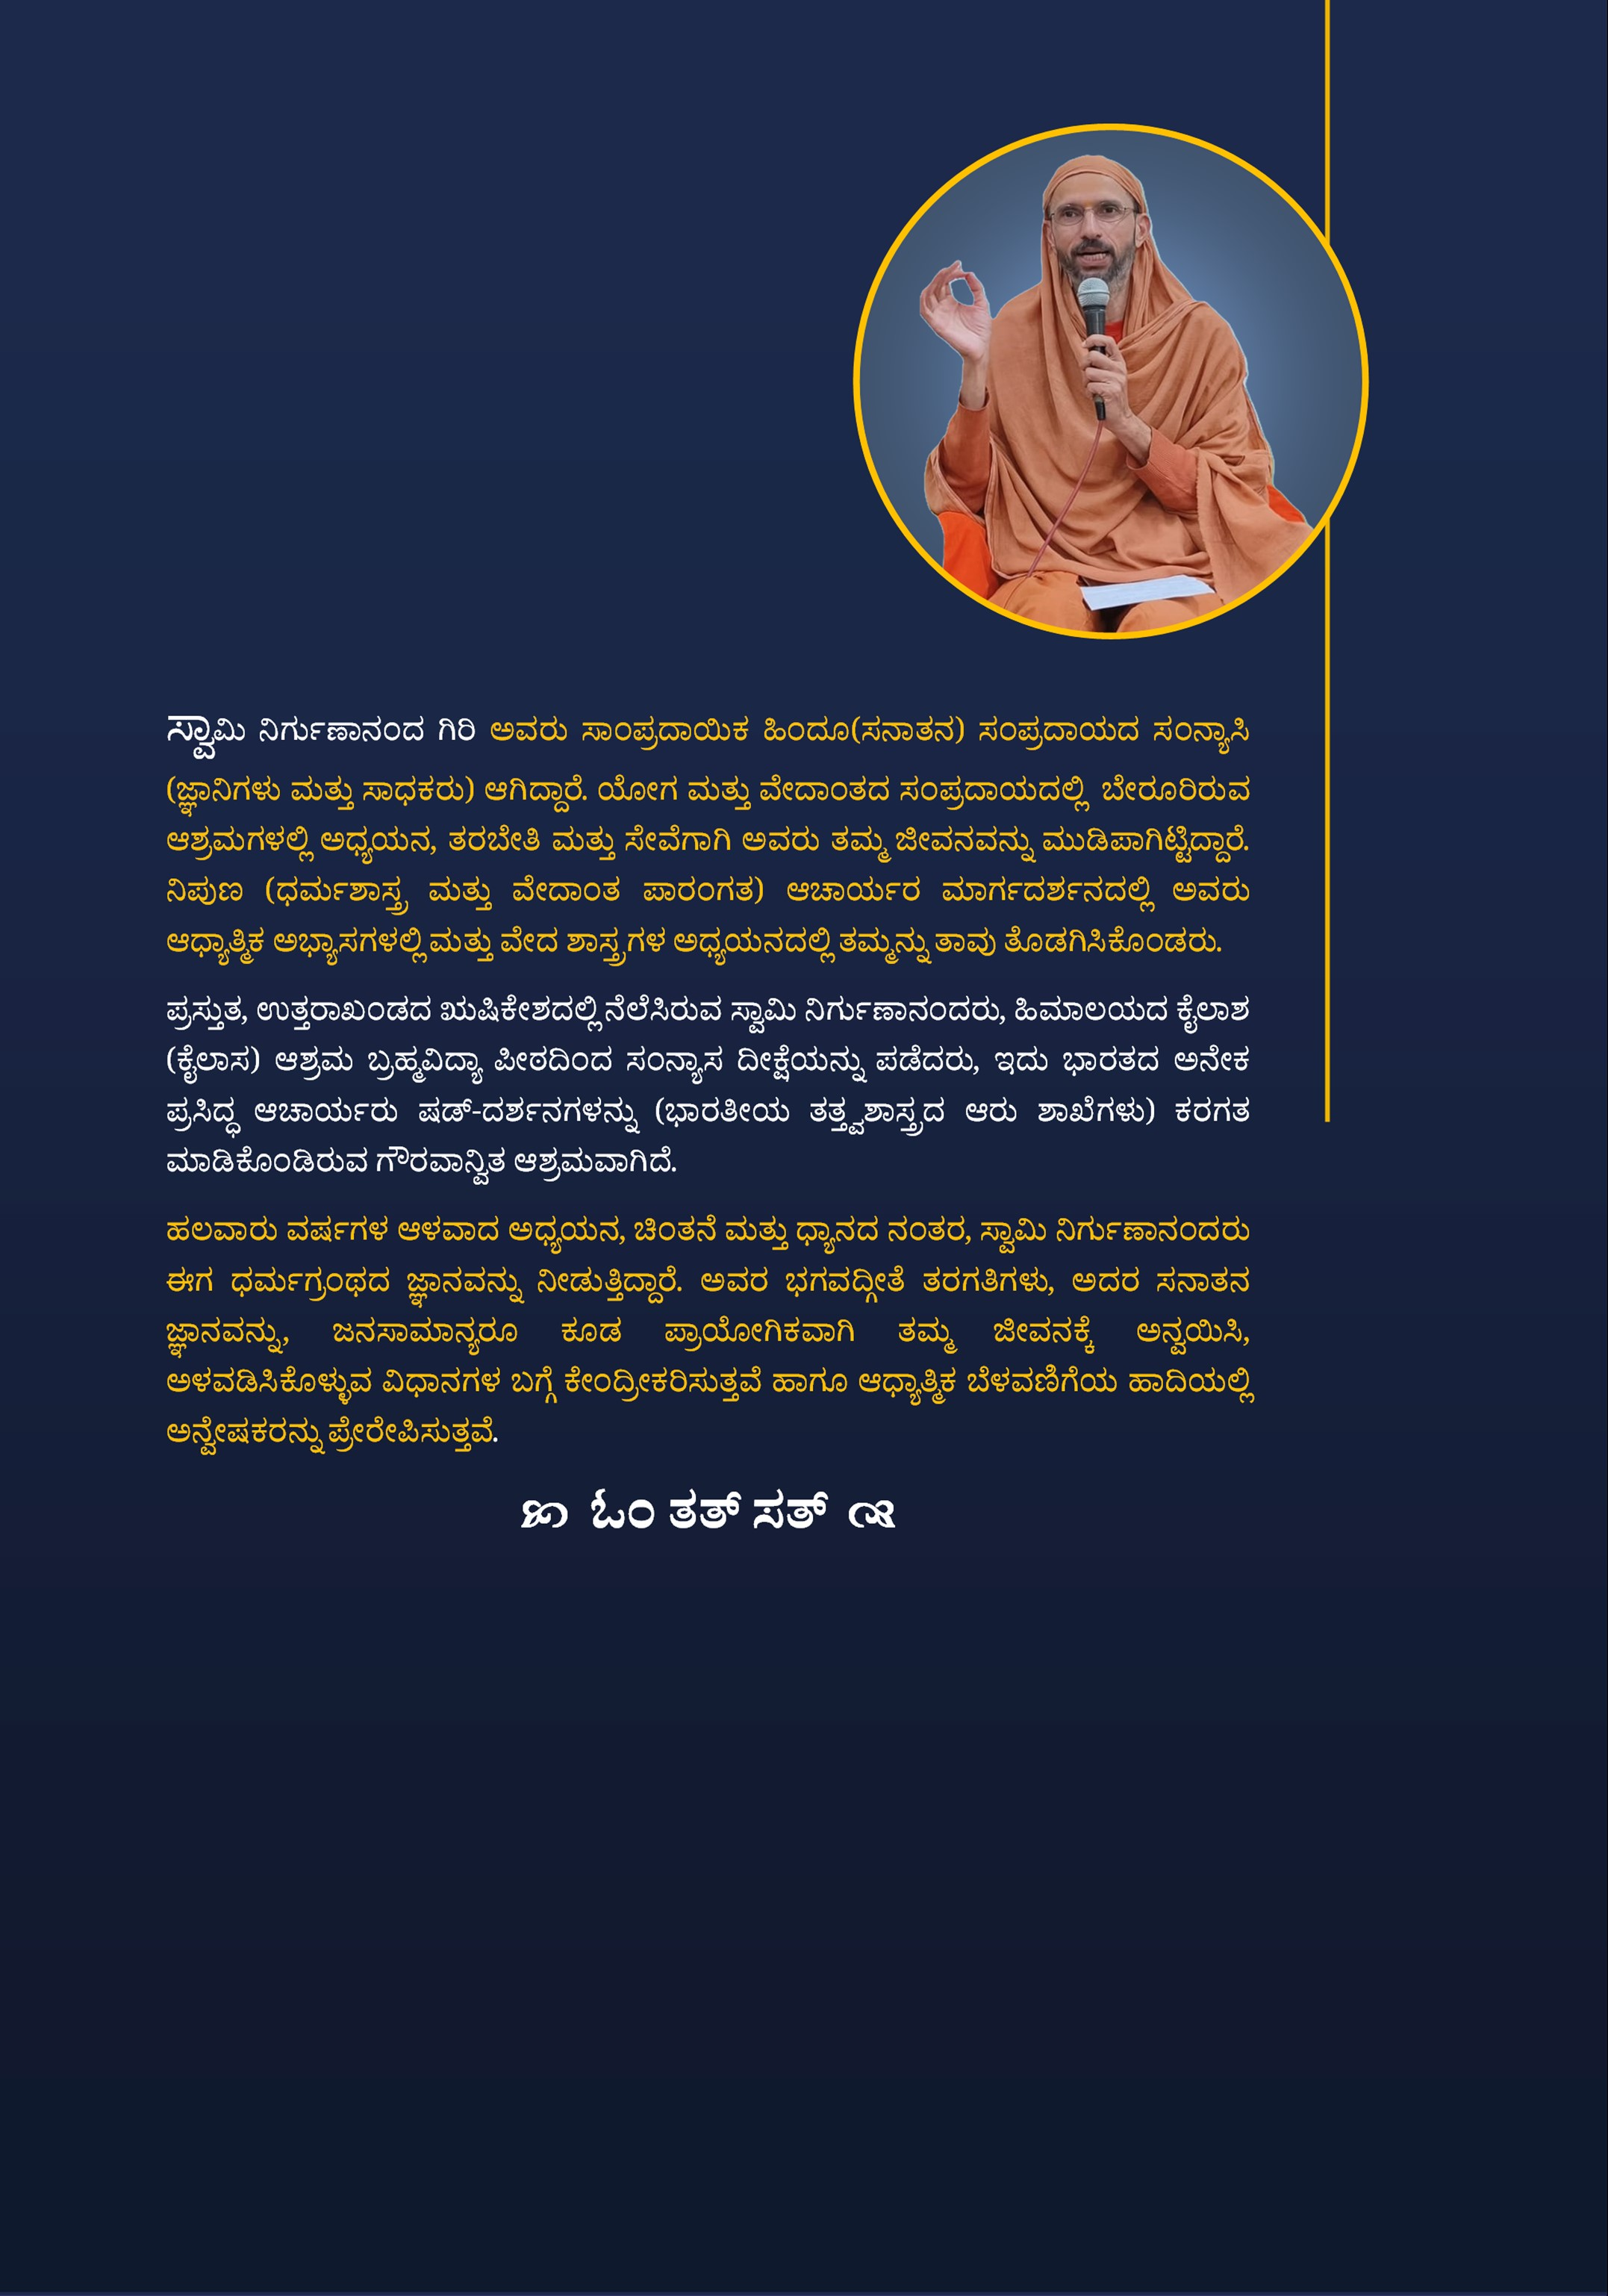
\includegraphics[width=\paperwidth,height=\paperheight]{./images/page02.jpg}%
    }%
	}
   \else% do nothing
   \AddToShipoutPictureBG*{%
    \AtPageLowerLeft{%
        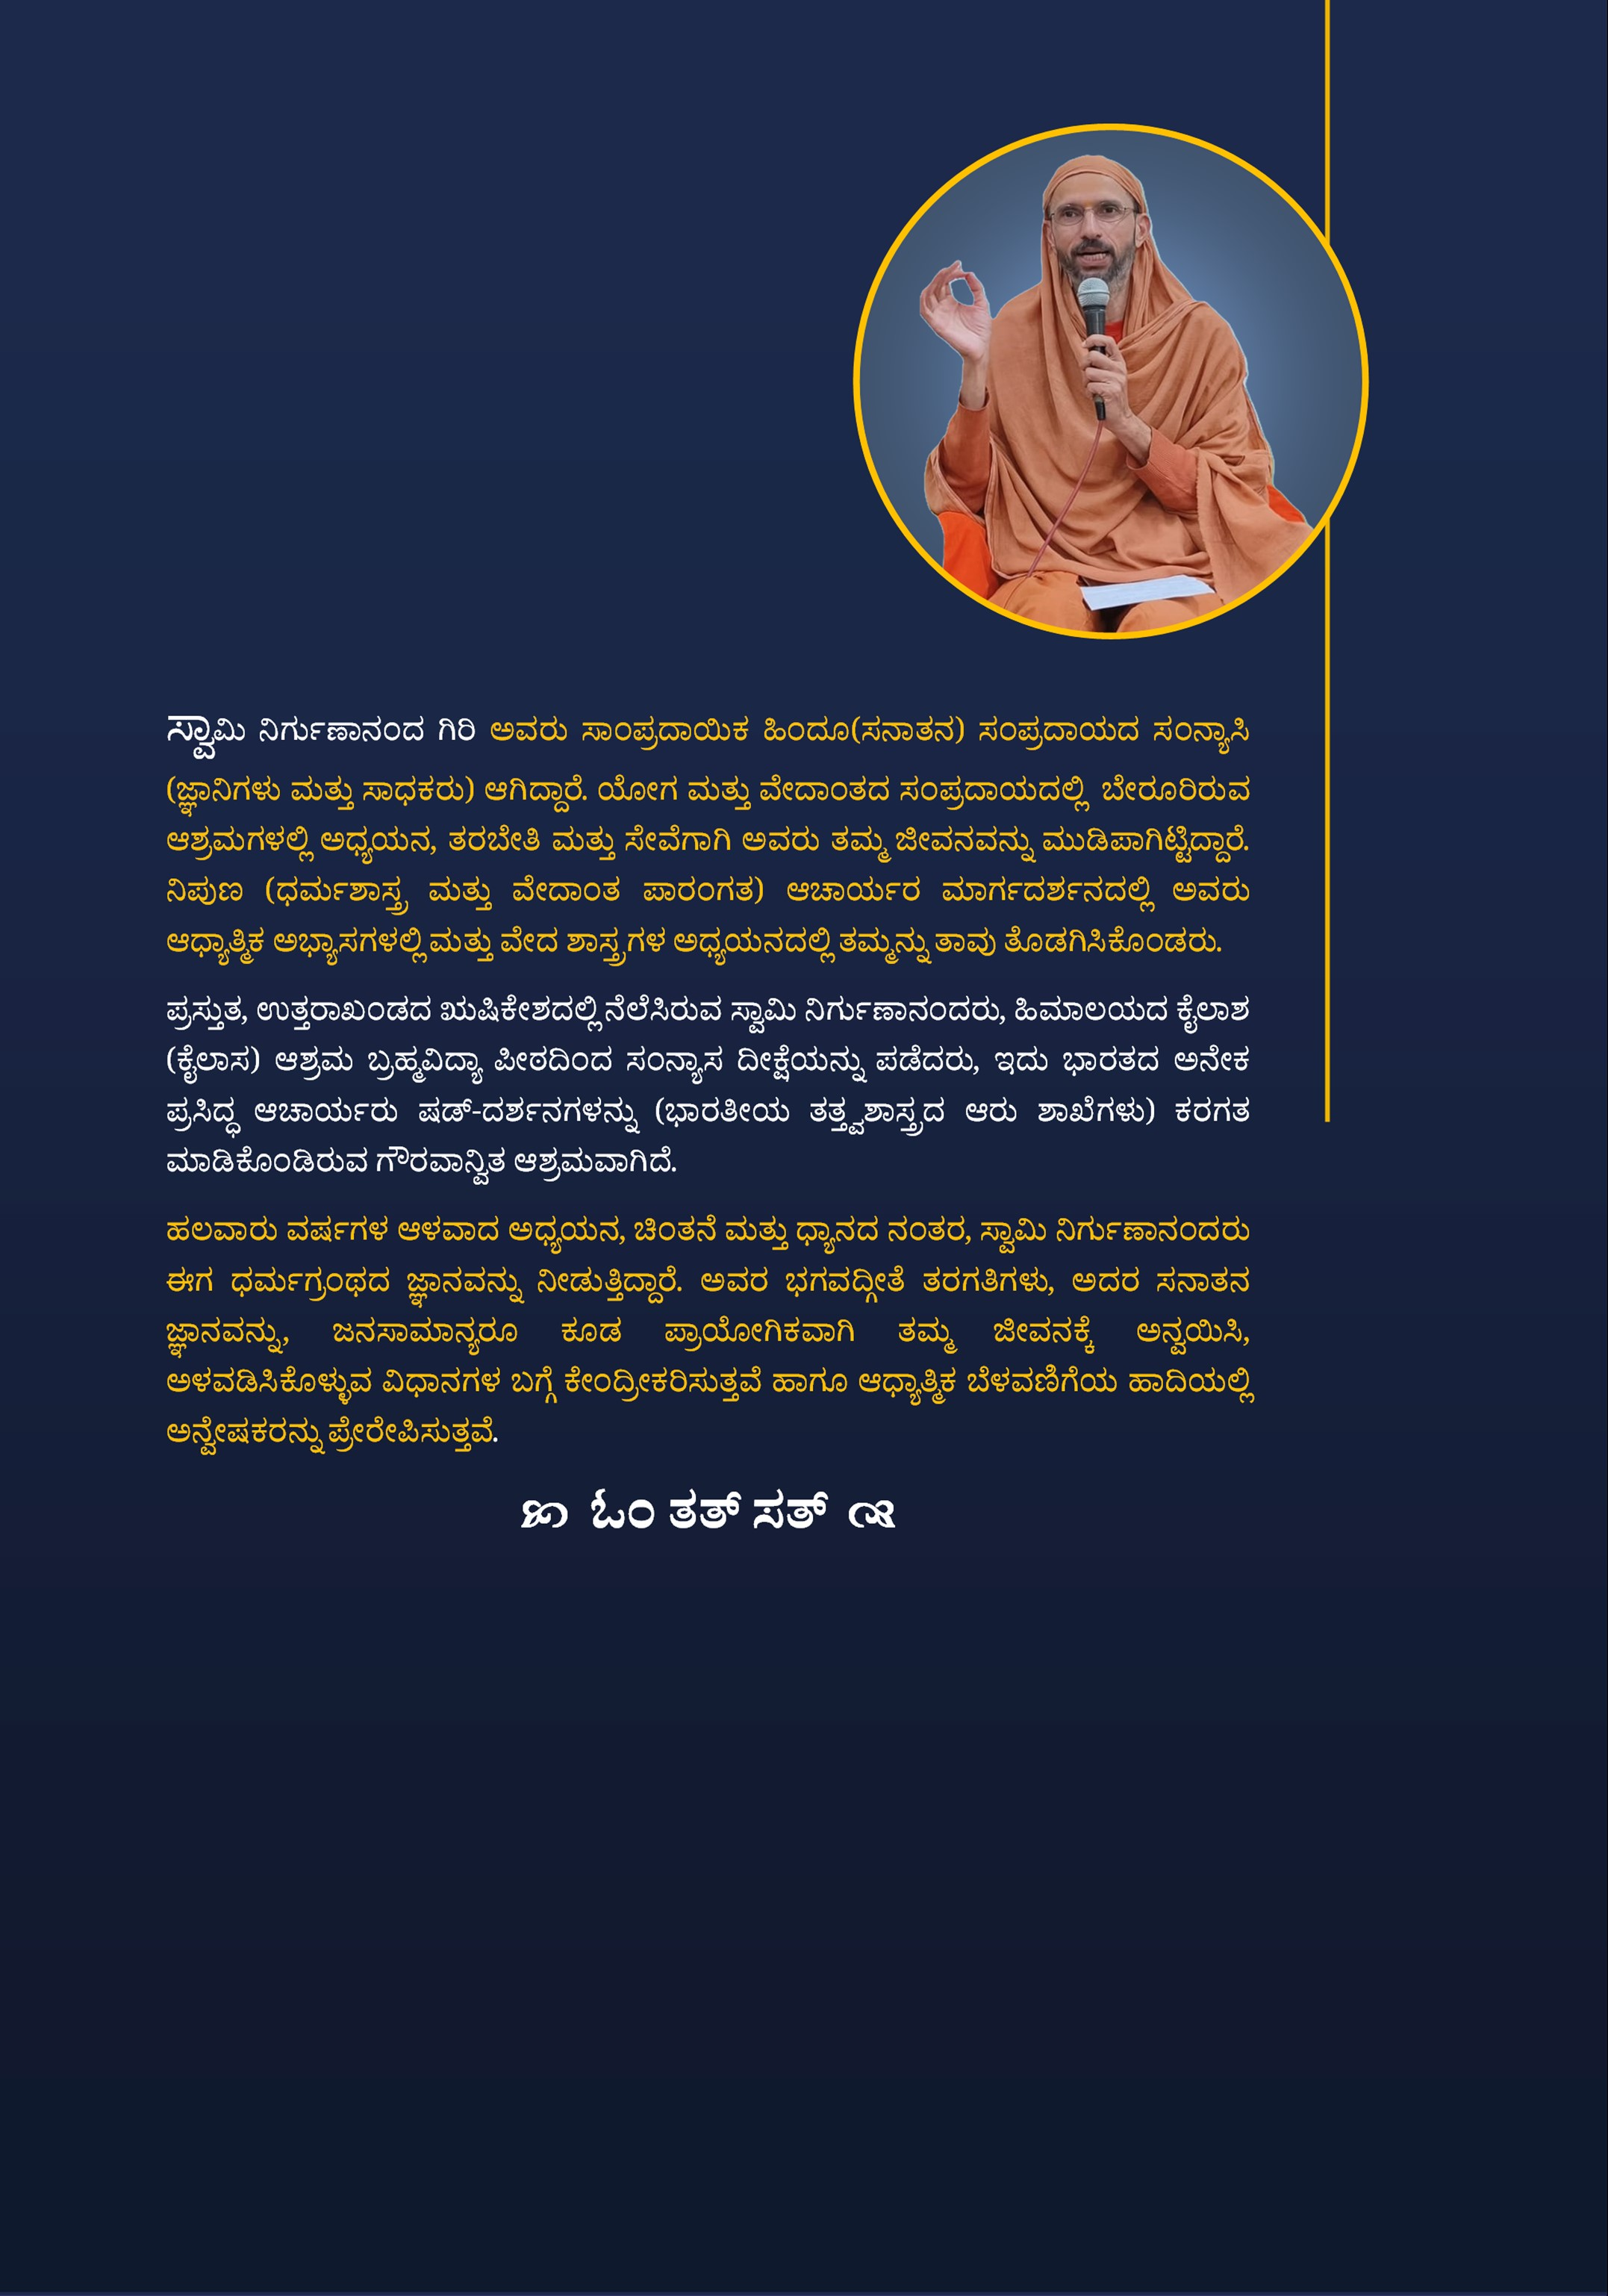
\includegraphics[width=\paperwidth,height=\paperheight]{./images/page02.jpg}%
    }%
	}
\fi
\begin{titlepage}
	%\pagecolor{pastelblue}
	\AddToShipoutPictureBG*{%
    \AtPageLowerLeft{%
        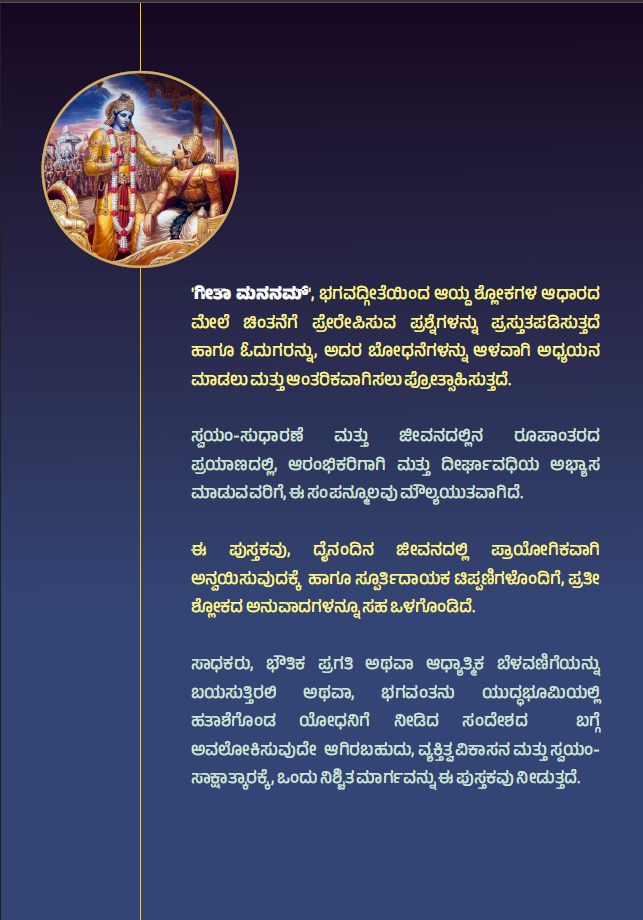
\includegraphics[width=\paperwidth,height=\paperheight]{./images/backcover.png}%
    }%
}
    \begin{center}
        \vspace*{0.5cm}
            
        {\Huge
        %\textbf{\color{white}\fontsize{50}{60}\selectfont ಗೀತಾ ಮನನಂ}
		}
        %\textbf{\\ \small \color{white}ದೈನಂದಿನ ಸ್ಪೂರ್ತಿ ಹಾಗೂ ಆತ್ಮಾವಲೋಕನಕ್ಕಾಗಿ}    
        \vspace{1.0cm}
            
        
		
            
        \vfill
            
        
            
        \vspace{0.1cm}
        {\color{white}    
		%\textbf{{\Large \mananamfont ಸ್ವಾಮಿ ನಿರ್ಗುಣಾನಂದ ಗಿರಿ}}\\
		%{\normalsize Swami Nirgunananda Giri\\Rishikesh, India}
        }
    \end{center}
\end{titlepage}
\nopagecolor% Use this to restore the color pages to white
\end{document}
